\documentclass[twoside]{book}

% Packages required by doxygen
\usepackage{fixltx2e}
\usepackage{calc}
\usepackage{doxygen}
\usepackage[export]{adjustbox} % also loads graphicx
\usepackage{graphicx}
\usepackage[utf8]{inputenc}
\usepackage{makeidx}
\usepackage{multicol}
\usepackage{multirow}
\PassOptionsToPackage{warn}{textcomp}
\usepackage{textcomp}
\usepackage[nointegrals]{wasysym}
\usepackage[table]{xcolor}

% Font selection
\usepackage[T1]{fontenc}
\usepackage[scaled=.90]{helvet}
\usepackage{courier}
\usepackage{amssymb}
\usepackage{sectsty}
\renewcommand{\familydefault}{\sfdefault}
\allsectionsfont{%
  \fontseries{bc}\selectfont%
  \color{darkgray}%
}
\renewcommand{\DoxyLabelFont}{%
  \fontseries{bc}\selectfont%
  \color{darkgray}%
}
\newcommand{\+}{\discretionary{\mbox{\scriptsize$\hookleftarrow$}}{}{}}

% Page & text layout
\usepackage{geometry}
\geometry{%
  a4paper,%
  top=2.5cm,%
  bottom=2.5cm,%
  left=2.5cm,%
  right=2.5cm%
}
\tolerance=750
\hfuzz=15pt
\hbadness=750
\setlength{\emergencystretch}{15pt}
\setlength{\parindent}{0cm}
\setlength{\parskip}{3ex plus 2ex minus 2ex}
\makeatletter
\renewcommand{\paragraph}{%
  \@startsection{paragraph}{4}{0ex}{-1.0ex}{1.0ex}{%
    \normalfont\normalsize\bfseries\SS@parafont%
  }%
}
\renewcommand{\subparagraph}{%
  \@startsection{subparagraph}{5}{0ex}{-1.0ex}{1.0ex}{%
    \normalfont\normalsize\bfseries\SS@subparafont%
  }%
}
\makeatother

% Headers & footers
\usepackage{fancyhdr}
\pagestyle{fancyplain}
\fancyhead[LE]{\fancyplain{}{\bfseries\thepage}}
\fancyhead[CE]{\fancyplain{}{}}
\fancyhead[RE]{\fancyplain{}{\bfseries\leftmark}}
\fancyhead[LO]{\fancyplain{}{\bfseries\rightmark}}
\fancyhead[CO]{\fancyplain{}{}}
\fancyhead[RO]{\fancyplain{}{\bfseries\thepage}}
\fancyfoot[LE]{\fancyplain{}{}}
\fancyfoot[CE]{\fancyplain{}{}}
\fancyfoot[RE]{\fancyplain{}{\bfseries\scriptsize Generated by Doxygen }}
\fancyfoot[LO]{\fancyplain{}{\bfseries\scriptsize Generated by Doxygen }}
\fancyfoot[CO]{\fancyplain{}{}}
\fancyfoot[RO]{\fancyplain{}{}}
\renewcommand{\footrulewidth}{0.4pt}
\renewcommand{\chaptermark}[1]{%
  \markboth{#1}{}%
}
\renewcommand{\sectionmark}[1]{%
  \markright{\thesection\ #1}%
}

% Indices & bibliography
\usepackage{natbib}
\usepackage[titles]{tocloft}
\setcounter{tocdepth}{3}
\setcounter{secnumdepth}{5}
\makeindex

% Hyperlinks (required, but should be loaded last)
\usepackage{ifpdf}
\ifpdf
  \usepackage[pdftex,pagebackref=true]{hyperref}
\else
  \usepackage[ps2pdf,pagebackref=true]{hyperref}
\fi
\hypersetup{%
  colorlinks=true,%
  linkcolor=blue,%
  citecolor=blue,%
  unicode%
}

% Custom commands
\newcommand{\clearemptydoublepage}{%
  \newpage{\pagestyle{empty}\cleardoublepage}%
}

\usepackage{caption}
\captionsetup{labelsep=space,justification=centering,font={bf},singlelinecheck=off,skip=4pt,position=top}

%===== C O N T E N T S =====

\begin{document}

% Titlepage & ToC
\hypersetup{pageanchor=false,
             bookmarksnumbered=true,
             pdfencoding=unicode
            }
\pagenumbering{alph}
\begin{titlepage}
\vspace*{7cm}
\begin{center}%
{\Large R\+WA Final Project \\[1ex]\large 1.\+0 }\\
\vspace*{1cm}
{\large Generated by Doxygen 1.8.13}\\
\end{center}
\end{titlepage}
\clearemptydoublepage
\pagenumbering{roman}
\tableofcontents
\clearemptydoublepage
\pagenumbering{arabic}
\hypersetup{pageanchor=true}

%--- Begin generated contents ---
\chapter{Class Index}
\section{Class List}
Here are the classes, structs, unions and interfaces with brief descriptions\+:\begin{DoxyCompactList}
\item\contentsline{section}{\hyperlink{structagvInfo}{agv\+Info} \\*A\+GV Information struct }{\pageref{structagvInfo}}{}
\item\contentsline{section}{\hyperlink{structall__Order}{all\+\_\+\+Order} \\*All order struct }{\pageref{structall__Order}}{}
\item\contentsline{section}{\hyperlink{classallStaticParts}{all\+Static\+Parts} \\*All\+Static\+Parts class }{\pageref{classallStaticParts}}{}
\item\contentsline{section}{\hyperlink{classBuildClass}{Build\+Class} \\*Build class }{\pageref{classBuildClass}}{}
\item\contentsline{section}{\hyperlink{classCompetition}{Competition} \\*\hyperlink{classCompetition}{Competition} class }{\pageref{classCompetition}}{}
\item\contentsline{section}{\hyperlink{classConveyerParts}{Conveyer\+Parts} \\*Conveyor parts class }{\pageref{classConveyerParts}}{}
\item\contentsline{section}{\hyperlink{classDetection}{Detection} \\*\hyperlink{classDetection}{Detection} class }{\pageref{classDetection}}{}
\item\contentsline{section}{\hyperlink{classGantryControl}{Gantry\+Control} \\*Gantry Control class }{\pageref{classGantryControl}}{}
\item\contentsline{section}{\hyperlink{classObstaclesInAisle}{Obstacles\+In\+Aisle} \\*\hyperlink{classObstaclesInAisle}{Obstacles\+In\+Aisle} class }{\pageref{classObstaclesInAisle}}{}
\item\contentsline{section}{\hyperlink{structOrder}{Order} \\*\hyperlink{structOrder}{Order} typedef }{\pageref{structOrder}}{}
\item\contentsline{section}{\hyperlink{structPart}{Part} \\*\hyperlink{structPart}{Part} typedef }{\pageref{structPart}}{}
\item\contentsline{section}{\hyperlink{structPosition}{Position} \\*\hyperlink{structPosition}{Position} typedef }{\pageref{structPosition}}{}
\item\contentsline{section}{\hyperlink{structPresetLocation}{Preset\+Location} \\*Preset Location typedef }{\pageref{structPresetLocation}}{}
\item\contentsline{section}{\hyperlink{structProduct}{Product} \\*\hyperlink{structProduct}{Product} typedef }{\pageref{structProduct}}{}
\item\contentsline{section}{\hyperlink{structShipment}{Shipment} \\*\hyperlink{structShipment}{Shipment} typedef }{\pageref{structShipment}}{}
\item\contentsline{section}{\hyperlink{structsimilarParts}{similar\+Parts} \\*Similar parts struct }{\pageref{structsimilarParts}}{}
\item\contentsline{section}{\hyperlink{structStats}{Stats} \\*\hyperlink{structStats}{Stats} typedef }{\pageref{structStats}}{}
\end{DoxyCompactList}

\chapter{File Index}
\section{File List}
Here is a list of all documented files with brief descriptions\+:\begin{DoxyCompactList}
\item\contentsline{section}{include/\hyperlink{competition_8h}{competition.\+h} \\*Starts the A\+R\+I\+AC competition }{\pageref{competition_8h}}{}
\item\contentsline{section}{include/{\bfseries conveyer.\+h} }{\pageref{conveyer_8h}}{}
\item\contentsline{section}{include/\hyperlink{gantry__control_8h}{gantry\+\_\+control.\+h} \\*Gantry class }{\pageref{gantry__control_8h}}{}
\item\contentsline{section}{include/\hyperlink{obstacles_8h}{obstacles.\+h} \\*\hyperlink{classObstaclesInAisle}{Obstacles\+In\+Aisle} class }{\pageref{obstacles_8h}}{}
\item\contentsline{section}{include/\hyperlink{orderBuild_8h}{order\+Build.\+h} \\*\hyperlink{classBuildClass}{Build\+Class} and \hyperlink{classallStaticParts}{all\+Static\+Parts} class }{\pageref{orderBuild_8h}}{}
\item\contentsline{section}{include/\hyperlink{utils_8h}{utils.\+h} \\*Contains general utility typedefs }{\pageref{utils_8h}}{}
\item\contentsline{section}{src/\hyperlink{competition_8cpp}{competition.\+cpp} \\*Starts the A\+R\+I\+AC competition }{\pageref{competition_8cpp}}{}
\item\contentsline{section}{src/\hyperlink{gantry__control_8cpp}{gantry\+\_\+control.\+cpp} \\*Implements the \hyperlink{classGantryControl}{Gantry\+Control} class methods }{\pageref{gantry__control_8cpp}}{}
\item\contentsline{section}{src/\hyperlink{obstacles_8cpp}{obstacles.\+cpp} \\*\hyperlink{classObstaclesInAisle}{Obstacles\+In\+Aisle} class methods implementation }{\pageref{obstacles_8cpp}}{}
\item\contentsline{section}{src/\hyperlink{orderBuild_8cpp}{order\+Build.\+cpp} \\*\hyperlink{classBuildClass}{Build\+Class} and \hyperlink{classallStaticParts}{all\+Static\+Parts} class implementation }{\pageref{orderBuild_8cpp}}{}
\item\contentsline{section}{src/\hyperlink{rwa__final__node_8cpp}{rwa\+\_\+final\+\_\+node.\+cpp} \\*Main file for rwa5 }{\pageref{rwa__final__node_8cpp}}{}
\item\contentsline{section}{src/\hyperlink{utils_8cpp}{utils.\+cpp} \\*Utility functions implementation }{\pageref{utils_8cpp}}{}
\end{DoxyCompactList}

\chapter{Class Documentation}
\hypertarget{structagvInfo}{}\section{agv\+Info Struct Reference}
\label{structagvInfo}\index{agv\+Info@{agv\+Info}}


A\+GV Information struct.  




{\ttfamily \#include $<$utils.\+h$>$}

\subsection*{Public Attributes}
\begin{DoxyCompactItemize}
\item 
\mbox{\Hypertarget{structagvInfo_a54c7918b537ffca61497ffcb0cd93180}\label{structagvInfo_a54c7918b537ffca61497ffcb0cd93180}} 
std\+::unordered\+\_\+map$<$ std\+::string, std\+::vector$<$ \hyperlink{structProduct}{Product} $>$ $>$ {\bfseries prod\+\_\+on\+\_\+tray}
\item 
\mbox{\Hypertarget{structagvInfo_abfeb16cd018edba83deb548706f9d18e}\label{structagvInfo_abfeb16cd018edba83deb548706f9d18e}} 
std\+::vector$<$ struct \hyperlink{structall__Order}{all\+\_\+\+Order} $\ast$ $>$ {\bfseries complete\+\_\+order\+\_\+data}
\item 
\mbox{\Hypertarget{structagvInfo_a98e263e9827fad038ca72e64fe959c63}\label{structagvInfo_a98e263e9827fad038ca72e64fe959c63}} 
int {\bfseries count} = 0
\end{DoxyCompactItemize}


\subsection{Detailed Description}
A\+GV Information struct. 

The documentation for this struct was generated from the following file\+:\begin{DoxyCompactItemize}
\item 
include/\hyperlink{utils_8h}{utils.\+h}\end{DoxyCompactItemize}

\hypertarget{structall__Order}{}\section{all\+\_\+\+Order Struct Reference}
\label{structall__Order}\index{all\+\_\+\+Order@{all\+\_\+\+Order}}


All order struct.  




{\ttfamily \#include $<$order\+Build.\+h$>$}



Collaboration diagram for all\+\_\+\+Order\+:\nopagebreak
\begin{figure}[H]
\begin{center}
\leavevmode
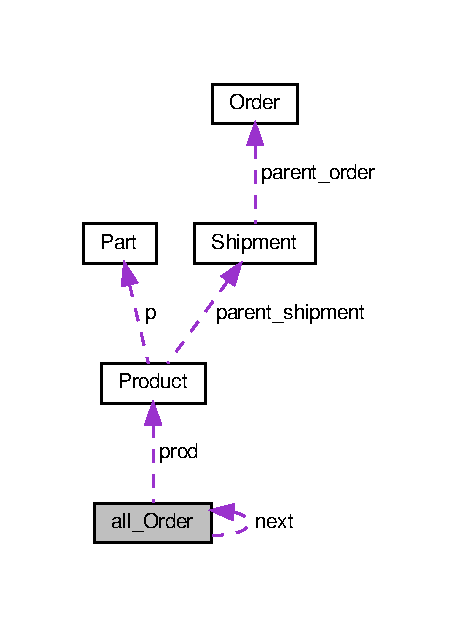
\includegraphics[width=221pt]{structall__Order__coll__graph}
\end{center}
\end{figure}
\subsection*{Public Attributes}
\begin{DoxyCompactItemize}
\item 
\mbox{\Hypertarget{structall__Order_abc229a6a4397223dda36c862d7a3b54c}\label{structall__Order_abc229a6a4397223dda36c862d7a3b54c}} 
\hyperlink{structProduct}{Product} {\bfseries prod}
\item 
\mbox{\Hypertarget{structall__Order_ad4b0a583424de97e7803edae8e163644}\label{structall__Order_ad4b0a583424de97e7803edae8e163644}} 
int {\bfseries ship\+\_\+num}
\item 
\mbox{\Hypertarget{structall__Order_a1f394679c4b09fab73b5e7b0284481a9}\label{structall__Order_a1f394679c4b09fab73b5e7b0284481a9}} 
std\+::string {\bfseries shipment\+\_\+type}
\item 
\mbox{\Hypertarget{structall__Order_a75278cdaa72ad356e1408c77a7d17c1c}\label{structall__Order_a75278cdaa72ad356e1408c77a7d17c1c}} 
bool {\bfseries priority} = false
\item 
\mbox{\Hypertarget{structall__Order_a27427252ea752809669ea6cafd3f334d}\label{structall__Order_a27427252ea752809669ea6cafd3f334d}} 
struct \hyperlink{structall__Order}{all\+\_\+\+Order} $\ast$ {\bfseries next}
\end{DoxyCompactItemize}


\subsection{Detailed Description}
All order struct. 

The documentation for this struct was generated from the following file\+:\begin{DoxyCompactItemize}
\item 
include/\hyperlink{orderBuild_8h}{order\+Build.\+h}\end{DoxyCompactItemize}

\hypertarget{classallStaticParts}{}\section{all\+Static\+Parts Class Reference}
\label{classallStaticParts}\index{all\+Static\+Parts@{all\+Static\+Parts}}


\hyperlink{classallStaticParts}{all\+Static\+Parts} class  




{\ttfamily \#include $<$order\+Build.\+h$>$}

\subsection*{Public Member Functions}
\begin{DoxyCompactItemize}
\item 
int \hyperlink{classallStaticParts_afcf48c7e1aacab3554bdc767e536d02b}{get\+Part} (\hyperlink{structProduct}{Product} \&prod)
\begin{DoxyCompactList}\small\item\em Gets part from product. \end{DoxyCompactList}\item 
void \hyperlink{classallStaticParts_aaf0ad01ce61050e4f1f91cd25ef13dc8}{set\+Part} (\hyperlink{structsimilarParts}{similar\+Parts} $\ast$data)
\begin{DoxyCompactList}\small\item\em Set part. \end{DoxyCompactList}\end{DoxyCompactItemize}


\subsection{Detailed Description}
\hyperlink{classallStaticParts}{all\+Static\+Parts} class 

\subsection{Member Function Documentation}
\mbox{\Hypertarget{classallStaticParts_afcf48c7e1aacab3554bdc767e536d02b}\label{classallStaticParts_afcf48c7e1aacab3554bdc767e536d02b}} 
\index{all\+Static\+Parts@{all\+Static\+Parts}!get\+Part@{get\+Part}}
\index{get\+Part@{get\+Part}!all\+Static\+Parts@{all\+Static\+Parts}}
\subsubsection{\texorpdfstring{get\+Part()}{getPart()}}
{\footnotesize\ttfamily int all\+Static\+Parts\+::get\+Part (\begin{DoxyParamCaption}\item[{\hyperlink{structProduct}{Product} \&}]{prod }\end{DoxyParamCaption})}



Gets part from product. 


\begin{DoxyParams}{Parameters}
{\em prod} & \hyperlink{structProduct}{Product} \\
\hline
\end{DoxyParams}
\begin{DoxyReturn}{Returns}
1 if product has part else 0 
\end{DoxyReturn}
\mbox{\Hypertarget{classallStaticParts_aaf0ad01ce61050e4f1f91cd25ef13dc8}\label{classallStaticParts_aaf0ad01ce61050e4f1f91cd25ef13dc8}} 
\index{all\+Static\+Parts@{all\+Static\+Parts}!set\+Part@{set\+Part}}
\index{set\+Part@{set\+Part}!all\+Static\+Parts@{all\+Static\+Parts}}
\subsubsection{\texorpdfstring{set\+Part()}{setPart()}}
{\footnotesize\ttfamily void all\+Static\+Parts\+::set\+Part (\begin{DoxyParamCaption}\item[{\hyperlink{structsimilarParts}{similar\+Parts} $\ast$}]{data }\end{DoxyParamCaption})}



Set part. 


\begin{DoxyParams}{Parameters}
{\em data} & Similar parts data \\
\hline
\end{DoxyParams}
\begin{DoxyReturn}{Returns}
None 
\end{DoxyReturn}


The documentation for this class was generated from the following files\+:\begin{DoxyCompactItemize}
\item 
include/\hyperlink{orderBuild_8h}{order\+Build.\+h}\item 
src/\hyperlink{orderBuild_8cpp}{order\+Build.\+cpp}\end{DoxyCompactItemize}

\hypertarget{classBuildClass}{}\section{Build\+Class Class Reference}
\label{classBuildClass}\index{Build\+Class@{Build\+Class}}


Build class.  




{\ttfamily \#include $<$order\+Build.\+h$>$}



Collaboration diagram for Build\+Class\+:\nopagebreak
\begin{figure}[H]
\begin{center}
\leavevmode
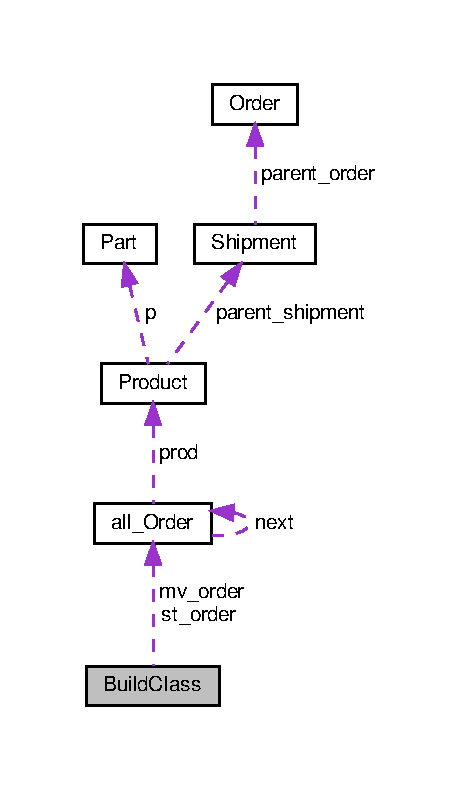
\includegraphics[width=221pt]{classBuildClass__coll__graph}
\end{center}
\end{figure}
\subsection*{Public Member Functions}
\begin{DoxyCompactItemize}
\item 
\hyperlink{classBuildClass_a03e935abdeb4b19d3e233dc6aa70f885}{Build\+Class} ()
\begin{DoxyCompactList}\small\item\em Constructor. \end{DoxyCompactList}\item 
void \hyperlink{classBuildClass_af3db7cdeb81f80f1b88f0cedb95d24e9}{order\+Callback} (const nist\+\_\+gear\+::\+Order \&ordermsg)
\begin{DoxyCompactList}\small\item\em \hyperlink{structOrder}{Order} Callback. \end{DoxyCompactList}\item 
void \hyperlink{classBuildClass_a7fa2d4355ca5ad8e2c26d82d5566d45e}{set\+List} (\hyperlink{structProduct}{Product} \&product\+\_\+received, int num\+\_\+shipment, std\+::string shipment\+\_\+type)
\begin{DoxyCompactList}\small\item\em Set List. \end{DoxyCompactList}\item 
struct \hyperlink{structall__Order}{all\+\_\+\+Order} $\ast$ \hyperlink{classBuildClass_afd4c97bb10d023ce4f6a6b15b88171a6}{get\+List} (\hyperlink{classConveyerParts}{Conveyer\+Parts} \&conveyer\+Parts\+Obj, int num\+\_\+obstacles)
\begin{DoxyCompactList}\small\item\em Get List function. \end{DoxyCompactList}\item 
void \hyperlink{classBuildClass_a64bc4cbe90399402e468f977e374f99e}{push\+List} (struct \hyperlink{structall__Order}{all\+\_\+\+Order} $\ast$prod)
\begin{DoxyCompactList}\small\item\em Push List. \end{DoxyCompactList}\item 
int \hyperlink{classBuildClass_acf20cc6dfbc979b0456b22a310627b42}{query\+Part} (\hyperlink{structProduct}{Product} \&prod)
\begin{DoxyCompactList}\small\item\em Query \hyperlink{structPart}{Part}. \end{DoxyCompactList}\item 
void \hyperlink{classBuildClass_a4d13438a582e88a6813385460d3c1a7f}{logical\+\_\+camera\+\_\+callback} (const nist\+\_\+gear\+::\+Logical\+Camera\+Image\+::\+Const\+Ptr \&msg, int cam\+\_\+id)
\begin{DoxyCompactList}\small\item\em Logical camera callback. \end{DoxyCompactList}\item 
void \hyperlink{classBuildClass_a5bcdfe5bfb567e511d397f02fd98e902}{shelf\+\_\+distance} ()
\begin{DoxyCompactList}\small\item\em Shelf Distance. \end{DoxyCompactList}\end{DoxyCompactItemize}
\subsection*{Public Attributes}
\begin{DoxyCompactItemize}
\item 
\mbox{\Hypertarget{classBuildClass_a4e780c195a7ef83b8a6d1b3561c30df9}\label{classBuildClass_a4e780c195a7ef83b8a6d1b3561c30df9}} 
bool \hyperlink{classBuildClass_a4e780c195a7ef83b8a6d1b3561c30df9}{agv1\+\_\+allocated} = false
\begin{DoxyCompactList}\small\item\em A\+G\+V1 Allocated. \end{DoxyCompactList}\item 
\mbox{\Hypertarget{classBuildClass_a2b9d524dd2f0409a722b60c039cda87f}\label{classBuildClass_a2b9d524dd2f0409a722b60c039cda87f}} 
bool \hyperlink{classBuildClass_a2b9d524dd2f0409a722b60c039cda87f}{agv2\+\_\+allocated} = false
\begin{DoxyCompactList}\small\item\em A\+G\+V2 Allocated. \end{DoxyCompactList}\item 
\mbox{\Hypertarget{classBuildClass_a5972aaddc18c4eeb901d6712abced0ad}\label{classBuildClass_a5972aaddc18c4eeb901d6712abced0ad}} 
bool \hyperlink{classBuildClass_a5972aaddc18c4eeb901d6712abced0ad}{order\+\_\+read} = false
\begin{DoxyCompactList}\small\item\em \hyperlink{structOrder}{Order} read. \end{DoxyCompactList}\item 
\mbox{\Hypertarget{classBuildClass_a54649e5a5dd731a0c11660d7f243033a}\label{classBuildClass_a54649e5a5dd731a0c11660d7f243033a}} 
std\+::vector$<$ \hyperlink{structOrder}{Order} $>$ \hyperlink{classBuildClass_a54649e5a5dd731a0c11660d7f243033a}{all\+Orders}
\begin{DoxyCompactList}\small\item\em All Orders array. \end{DoxyCompactList}\item 
\mbox{\Hypertarget{classBuildClass_ae03a5f1252946a467364d6424f604b75}\label{classBuildClass_ae03a5f1252946a467364d6424f604b75}} 
std\+::vector$<$ int $>$ \hyperlink{classBuildClass_ae03a5f1252946a467364d6424f604b75}{num\+\_\+prod\+\_\+in\+\_\+ship}
\begin{DoxyCompactList}\small\item\em Number of products in shipment. \end{DoxyCompactList}\item 
\mbox{\Hypertarget{classBuildClass_a46932efd4c8b2b97d0624a6117b40ee0}\label{classBuildClass_a46932efd4c8b2b97d0624a6117b40ee0}} 
std\+::unordered\+\_\+map$<$ int, int $>$ \hyperlink{classBuildClass_a46932efd4c8b2b97d0624a6117b40ee0}{ship\+\_\+build\+\_\+count}
\begin{DoxyCompactList}\small\item\em \hyperlink{structShipment}{Shipment} build count. \end{DoxyCompactList}\item 
\mbox{\Hypertarget{classBuildClass_afee9ec162b045de467138097c913ab3a}\label{classBuildClass_afee9ec162b045de467138097c913ab3a}} 
struct \hyperlink{structall__Order}{all\+\_\+\+Order} $\ast$ \hyperlink{classBuildClass_afee9ec162b045de467138097c913ab3a}{st\+\_\+order} = N\+U\+LL
\begin{DoxyCompactList}\small\item\em St order. \end{DoxyCompactList}\item 
\mbox{\Hypertarget{classBuildClass_a97f473aacf55fc9e2f036df24f14a5ad}\label{classBuildClass_a97f473aacf55fc9e2f036df24f14a5ad}} 
struct \hyperlink{structall__Order}{all\+\_\+\+Order} $\ast$ \hyperlink{classBuildClass_a97f473aacf55fc9e2f036df24f14a5ad}{mv\+\_\+order} = N\+U\+LL
\begin{DoxyCompactList}\small\item\em Mv order. \end{DoxyCompactList}\item 
\mbox{\Hypertarget{classBuildClass_a7a270922ce988fa65df7fd153eb32574}\label{classBuildClass_a7a270922ce988fa65df7fd153eb32574}} 
bool \hyperlink{classBuildClass_a7a270922ce988fa65df7fd153eb32574}{clear\+\_\+agv1} = false
\begin{DoxyCompactList}\small\item\em Clear A\+G\+V1. \end{DoxyCompactList}\item 
\mbox{\Hypertarget{classBuildClass_a152890ffd474645a17cd05a48e25d969}\label{classBuildClass_a152890ffd474645a17cd05a48e25d969}} 
bool \hyperlink{classBuildClass_a152890ffd474645a17cd05a48e25d969}{clear\+\_\+agv2} = false
\begin{DoxyCompactList}\small\item\em Clear A\+G\+V2. \end{DoxyCompactList}\item 
\mbox{\Hypertarget{classBuildClass_a347a5c88bc6562ea1c3be62cd9bb7ae1}\label{classBuildClass_a347a5c88bc6562ea1c3be62cd9bb7ae1}} 
std\+::string \hyperlink{classBuildClass_a347a5c88bc6562ea1c3be62cd9bb7ae1}{clear\+\_\+agv1\+\_\+for\+\_\+ship\+\_\+type} = \char`\"{}\char`\"{}
\begin{DoxyCompactList}\small\item\em Clear A\+G\+V1 for shipment type. \end{DoxyCompactList}\item 
\mbox{\Hypertarget{classBuildClass_a4f1d9c135fd347f4e88722a389017c25}\label{classBuildClass_a4f1d9c135fd347f4e88722a389017c25}} 
std\+::string \hyperlink{classBuildClass_a4f1d9c135fd347f4e88722a389017c25}{clear\+\_\+agv2\+\_\+for\+\_\+ship\+\_\+type} = \char`\"{}\char`\"{}
\begin{DoxyCompactList}\small\item\em Clear A\+G\+V2 for shipment type. \end{DoxyCompactList}\item 
\mbox{\Hypertarget{classBuildClass_ad9f54938ad08ac1e9b1902d8acde2448}\label{classBuildClass_ad9f54938ad08ac1e9b1902d8acde2448}} 
std\+::vector$<$ int $>$ \hyperlink{classBuildClass_ad9f54938ad08ac1e9b1902d8acde2448}{most\+\_\+recent\+\_\+order\+\_\+agv1}
\begin{DoxyCompactList}\small\item\em Most recent order agv1. \end{DoxyCompactList}\item 
\mbox{\Hypertarget{classBuildClass_a23919ef11440ca0d514f5b677b729cb7}\label{classBuildClass_a23919ef11440ca0d514f5b677b729cb7}} 
std\+::vector$<$ int $>$ \hyperlink{classBuildClass_a23919ef11440ca0d514f5b677b729cb7}{most\+\_\+recent\+\_\+order\+\_\+agv2}
\begin{DoxyCompactList}\small\item\em Most recent order agv2. \end{DoxyCompactList}\item 
\mbox{\Hypertarget{classBuildClass_ad2928c00304dde02561cdfd214f5ada2}\label{classBuildClass_ad2928c00304dde02561cdfd214f5ada2}} 
std\+::vector$<$ std\+::pair$<$ float, float $>$ $>$ \hyperlink{classBuildClass_ad2928c00304dde02561cdfd214f5ada2}{position\+Gap}
\begin{DoxyCompactList}\small\item\em \hyperlink{structPosition}{Position} Gap vector. \end{DoxyCompactList}\item 
\mbox{\Hypertarget{classBuildClass_a85c6af17d47644b2353b81dfc3399200}\label{classBuildClass_a85c6af17d47644b2353b81dfc3399200}} 
std\+::vector$<$ int $>$ \hyperlink{classBuildClass_a85c6af17d47644b2353b81dfc3399200}{gap\+Num}
\begin{DoxyCompactList}\small\item\em Gap Number. \end{DoxyCompactList}\end{DoxyCompactItemize}


\subsection{Detailed Description}
Build class. 

\subsection{Constructor \& Destructor Documentation}
\mbox{\Hypertarget{classBuildClass_a03e935abdeb4b19d3e233dc6aa70f885}\label{classBuildClass_a03e935abdeb4b19d3e233dc6aa70f885}} 
\index{Build\+Class@{Build\+Class}!Build\+Class@{Build\+Class}}
\index{Build\+Class@{Build\+Class}!Build\+Class@{Build\+Class}}
\subsubsection{\texorpdfstring{Build\+Class()}{BuildClass()}}
{\footnotesize\ttfamily Build\+Class\+::\+Build\+Class (\begin{DoxyParamCaption}{ }\end{DoxyParamCaption})\hspace{0.3cm}{\ttfamily [inline]}}



Constructor. 


\begin{DoxyParams}{Parameters}
{\em None} & None \\
\hline
\end{DoxyParams}
\begin{DoxyReturn}{Returns}
None 
\end{DoxyReturn}


\subsection{Member Function Documentation}
\mbox{\Hypertarget{classBuildClass_afd4c97bb10d023ce4f6a6b15b88171a6}\label{classBuildClass_afd4c97bb10d023ce4f6a6b15b88171a6}} 
\index{Build\+Class@{Build\+Class}!get\+List@{get\+List}}
\index{get\+List@{get\+List}!Build\+Class@{Build\+Class}}
\subsubsection{\texorpdfstring{get\+List()}{getList()}}
{\footnotesize\ttfamily struct \hyperlink{structall__Order}{all\+\_\+\+Order} $\ast$ Build\+Class\+::get\+List (\begin{DoxyParamCaption}\item[{\hyperlink{classConveyerParts}{Conveyer\+Parts} \&}]{conveyer\+Parts\+Obj,  }\item[{int}]{num\+\_\+obstacles }\end{DoxyParamCaption})}



Get List function. 


\begin{DoxyParams}{Parameters}
{\em conveyer\+Parts\+Obj} & Conveyor Parts Object \\
\hline
{\em num\+\_\+obstacles} & Number of obstacles \\
\hline
\end{DoxyParams}
\begin{DoxyReturn}{Returns}
All orders 
\end{DoxyReturn}
\mbox{\Hypertarget{classBuildClass_a4d13438a582e88a6813385460d3c1a7f}\label{classBuildClass_a4d13438a582e88a6813385460d3c1a7f}} 
\index{Build\+Class@{Build\+Class}!logical\+\_\+camera\+\_\+callback@{logical\+\_\+camera\+\_\+callback}}
\index{logical\+\_\+camera\+\_\+callback@{logical\+\_\+camera\+\_\+callback}!Build\+Class@{Build\+Class}}
\subsubsection{\texorpdfstring{logical\+\_\+camera\+\_\+callback()}{logical\_camera\_callback()}}
{\footnotesize\ttfamily void Build\+Class\+::logical\+\_\+camera\+\_\+callback (\begin{DoxyParamCaption}\item[{const nist\+\_\+gear\+::\+Logical\+Camera\+Image\+::\+Const\+Ptr \&}]{msg,  }\item[{int}]{cam\+\_\+id }\end{DoxyParamCaption})}



Logical camera callback. 


\begin{DoxyParams}{Parameters}
{\em msg} & Logical Camera Image \\
\hline
\end{DoxyParams}
\begin{DoxyReturn}{Returns}
None 
\end{DoxyReturn}
\mbox{\Hypertarget{classBuildClass_af3db7cdeb81f80f1b88f0cedb95d24e9}\label{classBuildClass_af3db7cdeb81f80f1b88f0cedb95d24e9}} 
\index{Build\+Class@{Build\+Class}!order\+Callback@{order\+Callback}}
\index{order\+Callback@{order\+Callback}!Build\+Class@{Build\+Class}}
\subsubsection{\texorpdfstring{order\+Callback()}{orderCallback()}}
{\footnotesize\ttfamily void Build\+Class\+::order\+Callback (\begin{DoxyParamCaption}\item[{const nist\+\_\+gear\+::\+Order \&}]{ordermsg }\end{DoxyParamCaption})}



\hyperlink{structOrder}{Order} Callback. 


\begin{DoxyParams}{Parameters}
{\em ordermsg} & \hyperlink{structOrder}{Order} message \\
\hline
\end{DoxyParams}
\begin{DoxyReturn}{Returns}
None 
\end{DoxyReturn}
\mbox{\Hypertarget{classBuildClass_a64bc4cbe90399402e468f977e374f99e}\label{classBuildClass_a64bc4cbe90399402e468f977e374f99e}} 
\index{Build\+Class@{Build\+Class}!push\+List@{push\+List}}
\index{push\+List@{push\+List}!Build\+Class@{Build\+Class}}
\subsubsection{\texorpdfstring{push\+List()}{pushList()}}
{\footnotesize\ttfamily void Build\+Class\+::push\+List (\begin{DoxyParamCaption}\item[{struct \hyperlink{structall__Order}{all\+\_\+\+Order} $\ast$}]{prod }\end{DoxyParamCaption})}



Push List. 


\begin{DoxyParams}{Parameters}
{\em prod} & \hyperlink{structProduct}{Product} \\
\hline
\end{DoxyParams}
\begin{DoxyReturn}{Returns}
None 
\end{DoxyReturn}
\mbox{\Hypertarget{classBuildClass_acf20cc6dfbc979b0456b22a310627b42}\label{classBuildClass_acf20cc6dfbc979b0456b22a310627b42}} 
\index{Build\+Class@{Build\+Class}!query\+Part@{query\+Part}}
\index{query\+Part@{query\+Part}!Build\+Class@{Build\+Class}}
\subsubsection{\texorpdfstring{query\+Part()}{queryPart()}}
{\footnotesize\ttfamily int Build\+Class\+::query\+Part (\begin{DoxyParamCaption}\item[{\hyperlink{structProduct}{Product} \&}]{prod }\end{DoxyParamCaption})}



Query \hyperlink{structPart}{Part}. 


\begin{DoxyParams}{Parameters}
{\em prod} & \hyperlink{structProduct}{Product} \\
\hline
\end{DoxyParams}
\begin{DoxyReturn}{Returns}
\hyperlink{structPart}{Part} number 
\end{DoxyReturn}
\mbox{\Hypertarget{classBuildClass_a7fa2d4355ca5ad8e2c26d82d5566d45e}\label{classBuildClass_a7fa2d4355ca5ad8e2c26d82d5566d45e}} 
\index{Build\+Class@{Build\+Class}!set\+List@{set\+List}}
\index{set\+List@{set\+List}!Build\+Class@{Build\+Class}}
\subsubsection{\texorpdfstring{set\+List()}{setList()}}
{\footnotesize\ttfamily void Build\+Class\+::set\+List (\begin{DoxyParamCaption}\item[{\hyperlink{structProduct}{Product} \&}]{product\+\_\+received,  }\item[{int}]{num\+\_\+shipment,  }\item[{std\+::string}]{shipment\+\_\+type }\end{DoxyParamCaption})}



Set List. 


\begin{DoxyParams}{Parameters}
{\em product\+\_\+received} & \hyperlink{structProduct}{Product} recieved \\
\hline
{\em num\+\_\+shipment} & \hyperlink{structShipment}{Shipment} number \\
\hline
{\em shipment\+\_\+type} & \hyperlink{structShipment}{Shipment} type \\
\hline
\end{DoxyParams}
\begin{DoxyReturn}{Returns}
None 
\end{DoxyReturn}
\mbox{\Hypertarget{classBuildClass_a5bcdfe5bfb567e511d397f02fd98e902}\label{classBuildClass_a5bcdfe5bfb567e511d397f02fd98e902}} 
\index{Build\+Class@{Build\+Class}!shelf\+\_\+distance@{shelf\+\_\+distance}}
\index{shelf\+\_\+distance@{shelf\+\_\+distance}!Build\+Class@{Build\+Class}}
\subsubsection{\texorpdfstring{shelf\+\_\+distance()}{shelf\_distance()}}
{\footnotesize\ttfamily void Build\+Class\+::shelf\+\_\+distance (\begin{DoxyParamCaption}{ }\end{DoxyParamCaption})}



Shelf Distance. 


\begin{DoxyParams}{Parameters}
{\em None} & None \\
\hline
\end{DoxyParams}
\begin{DoxyReturn}{Returns}
None 
\end{DoxyReturn}


The documentation for this class was generated from the following files\+:\begin{DoxyCompactItemize}
\item 
include/\hyperlink{orderBuild_8h}{order\+Build.\+h}\item 
src/\hyperlink{orderBuild_8cpp}{order\+Build.\+cpp}\end{DoxyCompactItemize}

\hypertarget{classCompetition}{}\section{Competition Class Reference}
\label{classCompetition}\index{Competition@{Competition}}


\hyperlink{classCompetition}{Competition} class.  




{\ttfamily \#include $<$competition.\+h$>$}

\subsection*{Public Member Functions}
\begin{DoxyCompactItemize}
\item 
\hyperlink{classCompetition_a3d8b50d07d2424bd18743148237da31c}{Competition} (ros\+::\+Node\+Handle \&node)
\begin{DoxyCompactList}\small\item\em Constructor. \end{DoxyCompactList}\item 
void \hyperlink{classCompetition_af5400538e024248fc99f83cf26ca2f23}{init} ()
\begin{DoxyCompactList}\small\item\em Initialization function. \end{DoxyCompactList}\item 
void \hyperlink{classCompetition_a2505fb69a74ff70530c033c144f7f024}{start\+Competition} ()
\begin{DoxyCompactList}\small\item\em Starts the competition. \end{DoxyCompactList}\item 
void \hyperlink{classCompetition_a894a450b89f8d61d83f02f221fb1b0eb}{end\+Competition} ()
\begin{DoxyCompactList}\small\item\em Ends the competition. \end{DoxyCompactList}\item 
void \hyperlink{classCompetition_a0f5358904edd5675f14fc378b217f3f9}{ship\+Agv} (std\+::string agv, std\+::string ship\+\_\+type)
\begin{DoxyCompactList}\small\item\em Sends A\+GV to complete order. \end{DoxyCompactList}\item 
void \hyperlink{classCompetition_a1b9545e863fc4574b29b1e43e80ebda3}{competition\+\_\+state\+\_\+callback} (const std\+\_\+msgs\+::\+String\+::\+Const\+Ptr \&msg)
\begin{DoxyCompactList}\small\item\em \hyperlink{classCompetition}{Competition} state callback. \end{DoxyCompactList}\item 
void \hyperlink{classCompetition_ae4695e5697587f7af4aa40ebae953534}{competition\+\_\+clock\+\_\+callback} (const rosgraph\+\_\+msgs\+::\+Clock\+::\+Const\+Ptr \&msg)
\begin{DoxyCompactList}\small\item\em \hyperlink{classCompetition}{Competition} clock callback. \end{DoxyCompactList}\item 
void \hyperlink{classCompetition_a6f51ab2e5a0da50fc53035f3ff6c9c31}{order\+\_\+callback} (const nist\+\_\+gear\+::\+Order\+::\+Const\+Ptr \&msg)
\begin{DoxyCompactList}\small\item\em \hyperlink{structOrder}{Order} callback. \end{DoxyCompactList}\item 
double \hyperlink{classCompetition_a4ea6b45be32e5b0e1f8e72fc053c4550}{get\+Clock} ()
\begin{DoxyCompactList}\small\item\em Gets the competition time elapsed. \end{DoxyCompactList}\item 
double \hyperlink{classCompetition_a9c8b79a8c4a7bcc5eaa77a327df3f98a}{get\+Start\+Time} ()
\begin{DoxyCompactList}\small\item\em Gets the start time. \end{DoxyCompactList}\item 
std\+::string \hyperlink{classCompetition_a3c553faa38b1bc1fa6efa049c8e23735}{get\+Competition\+State} ()
\begin{DoxyCompactList}\small\item\em Gets the competition state. \end{DoxyCompactList}\item 
\hyperlink{utils_8h_abd807f196b951c0cdd24d50164d54763}{stats} \hyperlink{classCompetition_acb4ec20a6365fbb922bd20fc3509ddf8}{get\+Stats} (std\+::string function)
\begin{DoxyCompactList}\small\item\em Gets the competition stats. \end{DoxyCompactList}\end{DoxyCompactItemize}
\subsection*{Public Attributes}
\begin{DoxyCompactItemize}
\item 
std\+::unordered\+\_\+map$<$ std\+::string, std\+::string $>$ \hyperlink{classCompetition_a29e55fbb84b665c374f53113cf3fa2ca}{agv\+\_\+ship\+\_\+data}
\begin{DoxyCompactList}\small\item\em Gets the A\+GV shipment data. \end{DoxyCompactList}\end{DoxyCompactItemize}


\subsection{Detailed Description}
\hyperlink{classCompetition}{Competition} class. 

\subsection{Constructor \& Destructor Documentation}
\mbox{\Hypertarget{classCompetition_a3d8b50d07d2424bd18743148237da31c}\label{classCompetition_a3d8b50d07d2424bd18743148237da31c}} 
\index{Competition@{Competition}!Competition@{Competition}}
\index{Competition@{Competition}!Competition@{Competition}}
\subsubsection{\texorpdfstring{Competition()}{Competition()}}
{\footnotesize\ttfamily Competition\+::\+Competition (\begin{DoxyParamCaption}\item[{ros\+::\+Node\+Handle \&}]{node }\end{DoxyParamCaption})\hspace{0.3cm}{\ttfamily [explicit]}}



Constructor. 


\begin{DoxyParams}{Parameters}
{\em node} & R\+OS nodehandle \\
\hline
\end{DoxyParams}
\begin{DoxyReturn}{Returns}
None 
\end{DoxyReturn}


\subsection{Member Function Documentation}
\mbox{\Hypertarget{classCompetition_ae4695e5697587f7af4aa40ebae953534}\label{classCompetition_ae4695e5697587f7af4aa40ebae953534}} 
\index{Competition@{Competition}!competition\+\_\+clock\+\_\+callback@{competition\+\_\+clock\+\_\+callback}}
\index{competition\+\_\+clock\+\_\+callback@{competition\+\_\+clock\+\_\+callback}!Competition@{Competition}}
\subsubsection{\texorpdfstring{competition\+\_\+clock\+\_\+callback()}{competition\_clock\_callback()}}
{\footnotesize\ttfamily void Competition\+::competition\+\_\+clock\+\_\+callback (\begin{DoxyParamCaption}\item[{const rosgraph\+\_\+msgs\+::\+Clock\+::\+Const\+Ptr \&}]{msg }\end{DoxyParamCaption})}



\hyperlink{classCompetition}{Competition} clock callback. 

Called when a new message is received.


\begin{DoxyParams}{Parameters}
{\em msg} & Contain simulation time elapsed \\
\hline
\end{DoxyParams}
\begin{DoxyReturn}{Returns}
None 
\end{DoxyReturn}
\mbox{\Hypertarget{classCompetition_a1b9545e863fc4574b29b1e43e80ebda3}\label{classCompetition_a1b9545e863fc4574b29b1e43e80ebda3}} 
\index{Competition@{Competition}!competition\+\_\+state\+\_\+callback@{competition\+\_\+state\+\_\+callback}}
\index{competition\+\_\+state\+\_\+callback@{competition\+\_\+state\+\_\+callback}!Competition@{Competition}}
\subsubsection{\texorpdfstring{competition\+\_\+state\+\_\+callback()}{competition\_state\_callback()}}
{\footnotesize\ttfamily void Competition\+::competition\+\_\+state\+\_\+callback (\begin{DoxyParamCaption}\item[{const std\+\_\+msgs\+::\+String\+::\+Const\+Ptr \&}]{msg }\end{DoxyParamCaption})}



\hyperlink{classCompetition}{Competition} state callback. 

Called when a new message is received.


\begin{DoxyParams}{Parameters}
{\em msg} & Contains competition state \\
\hline
\end{DoxyParams}
\begin{DoxyReturn}{Returns}
None 
\end{DoxyReturn}
\mbox{\Hypertarget{classCompetition_a894a450b89f8d61d83f02f221fb1b0eb}\label{classCompetition_a894a450b89f8d61d83f02f221fb1b0eb}} 
\index{Competition@{Competition}!end\+Competition@{end\+Competition}}
\index{end\+Competition@{end\+Competition}!Competition@{Competition}}
\subsubsection{\texorpdfstring{end\+Competition()}{endCompetition()}}
{\footnotesize\ttfamily void Competition\+::end\+Competition (\begin{DoxyParamCaption}{ }\end{DoxyParamCaption})}



Ends the competition. 


\begin{DoxyParams}{Parameters}
{\em None} & \\
\hline
\end{DoxyParams}
\begin{DoxyReturn}{Returns}
None 
\end{DoxyReturn}
\mbox{\Hypertarget{classCompetition_a4ea6b45be32e5b0e1f8e72fc053c4550}\label{classCompetition_a4ea6b45be32e5b0e1f8e72fc053c4550}} 
\index{Competition@{Competition}!get\+Clock@{get\+Clock}}
\index{get\+Clock@{get\+Clock}!Competition@{Competition}}
\subsubsection{\texorpdfstring{get\+Clock()}{getClock()}}
{\footnotesize\ttfamily double Competition\+::get\+Clock (\begin{DoxyParamCaption}{ }\end{DoxyParamCaption})}



Gets the competition time elapsed. 


\begin{DoxyParams}{Parameters}
{\em None} & \\
\hline
\end{DoxyParams}
\begin{DoxyReturn}{Returns}
Time elapsed 
\end{DoxyReturn}
\mbox{\Hypertarget{classCompetition_a3c553faa38b1bc1fa6efa049c8e23735}\label{classCompetition_a3c553faa38b1bc1fa6efa049c8e23735}} 
\index{Competition@{Competition}!get\+Competition\+State@{get\+Competition\+State}}
\index{get\+Competition\+State@{get\+Competition\+State}!Competition@{Competition}}
\subsubsection{\texorpdfstring{get\+Competition\+State()}{getCompetitionState()}}
{\footnotesize\ttfamily std\+::string Competition\+::get\+Competition\+State (\begin{DoxyParamCaption}{ }\end{DoxyParamCaption})}



Gets the competition state. 


\begin{DoxyParams}{Parameters}
{\em None} & \\
\hline
\end{DoxyParams}
\begin{DoxyReturn}{Returns}
\hyperlink{classCompetition}{Competition} state 
\end{DoxyReturn}
\mbox{\Hypertarget{classCompetition_a9c8b79a8c4a7bcc5eaa77a327df3f98a}\label{classCompetition_a9c8b79a8c4a7bcc5eaa77a327df3f98a}} 
\index{Competition@{Competition}!get\+Start\+Time@{get\+Start\+Time}}
\index{get\+Start\+Time@{get\+Start\+Time}!Competition@{Competition}}
\subsubsection{\texorpdfstring{get\+Start\+Time()}{getStartTime()}}
{\footnotesize\ttfamily double Competition\+::get\+Start\+Time (\begin{DoxyParamCaption}{ }\end{DoxyParamCaption})}



Gets the start time. 


\begin{DoxyParams}{Parameters}
{\em None} & \\
\hline
\end{DoxyParams}
\begin{DoxyReturn}{Returns}
\hyperlink{classCompetition}{Competition} start time 
\end{DoxyReturn}
\mbox{\Hypertarget{classCompetition_acb4ec20a6365fbb922bd20fc3509ddf8}\label{classCompetition_acb4ec20a6365fbb922bd20fc3509ddf8}} 
\index{Competition@{Competition}!get\+Stats@{get\+Stats}}
\index{get\+Stats@{get\+Stats}!Competition@{Competition}}
\subsubsection{\texorpdfstring{get\+Stats()}{getStats()}}
{\footnotesize\ttfamily \hyperlink{utils_8h_abd807f196b951c0cdd24d50164d54763}{stats} Competition\+::get\+Stats (\begin{DoxyParamCaption}\item[{std\+::string}]{function }\end{DoxyParamCaption})}



Gets the competition stats. 


\begin{DoxyParams}{Parameters}
{\em function} & Function \\
\hline
\end{DoxyParams}
\begin{DoxyReturn}{Returns}
\hyperlink{classCompetition}{Competition} stats 
\end{DoxyReturn}
\mbox{\Hypertarget{classCompetition_af5400538e024248fc99f83cf26ca2f23}\label{classCompetition_af5400538e024248fc99f83cf26ca2f23}} 
\index{Competition@{Competition}!init@{init}}
\index{init@{init}!Competition@{Competition}}
\subsubsection{\texorpdfstring{init()}{init()}}
{\footnotesize\ttfamily void Competition\+::init (\begin{DoxyParamCaption}{ }\end{DoxyParamCaption})}



Initialization function. 


\begin{DoxyParams}{Parameters}
{\em None} & \\
\hline
\end{DoxyParams}
\begin{DoxyReturn}{Returns}
None 
\end{DoxyReturn}
\mbox{\Hypertarget{classCompetition_a6f51ab2e5a0da50fc53035f3ff6c9c31}\label{classCompetition_a6f51ab2e5a0da50fc53035f3ff6c9c31}} 
\index{Competition@{Competition}!order\+\_\+callback@{order\+\_\+callback}}
\index{order\+\_\+callback@{order\+\_\+callback}!Competition@{Competition}}
\subsubsection{\texorpdfstring{order\+\_\+callback()}{order\_callback()}}
{\footnotesize\ttfamily void Competition\+::order\+\_\+callback (\begin{DoxyParamCaption}\item[{const nist\+\_\+gear\+::\+Order\+::\+Const\+Ptr \&}]{msg }\end{DoxyParamCaption})}



\hyperlink{structOrder}{Order} callback. 


\begin{DoxyParams}{Parameters}
{\em msg} & Contains order number \\
\hline
\end{DoxyParams}
\begin{DoxyReturn}{Returns}
None 
\end{DoxyReturn}
\mbox{\Hypertarget{classCompetition_a0f5358904edd5675f14fc378b217f3f9}\label{classCompetition_a0f5358904edd5675f14fc378b217f3f9}} 
\index{Competition@{Competition}!ship\+Agv@{ship\+Agv}}
\index{ship\+Agv@{ship\+Agv}!Competition@{Competition}}
\subsubsection{\texorpdfstring{ship\+Agv()}{shipAgv()}}
{\footnotesize\ttfamily void Competition\+::ship\+Agv (\begin{DoxyParamCaption}\item[{std\+::string}]{agv,  }\item[{std\+::string}]{ship\+\_\+type }\end{DoxyParamCaption})}



Sends A\+GV to complete order. 


\begin{DoxyParams}{Parameters}
{\em agv} & A\+GV Number \\
\hline
{\em ship\+\_\+type} & \hyperlink{structShipment}{Shipment} type \\
\hline
\end{DoxyParams}
\begin{DoxyReturn}{Returns}
None 
\end{DoxyReturn}
\mbox{\Hypertarget{classCompetition_a2505fb69a74ff70530c033c144f7f024}\label{classCompetition_a2505fb69a74ff70530c033c144f7f024}} 
\index{Competition@{Competition}!start\+Competition@{start\+Competition}}
\index{start\+Competition@{start\+Competition}!Competition@{Competition}}
\subsubsection{\texorpdfstring{start\+Competition()}{startCompetition()}}
{\footnotesize\ttfamily void Competition\+::start\+Competition (\begin{DoxyParamCaption}{ }\end{DoxyParamCaption})}



Starts the competition. 


\begin{DoxyParams}{Parameters}
{\em None} & \\
\hline
\end{DoxyParams}
\begin{DoxyReturn}{Returns}
None 
\end{DoxyReturn}


\subsection{Member Data Documentation}
\mbox{\Hypertarget{classCompetition_a29e55fbb84b665c374f53113cf3fa2ca}\label{classCompetition_a29e55fbb84b665c374f53113cf3fa2ca}} 
\index{Competition@{Competition}!agv\+\_\+ship\+\_\+data@{agv\+\_\+ship\+\_\+data}}
\index{agv\+\_\+ship\+\_\+data@{agv\+\_\+ship\+\_\+data}!Competition@{Competition}}
\subsubsection{\texorpdfstring{agv\+\_\+ship\+\_\+data}{agv\_ship\_data}}
{\footnotesize\ttfamily std\+::unordered\+\_\+map$<$ std\+::string, std\+::string$>$ Competition\+::agv\+\_\+ship\+\_\+data}



Gets the A\+GV shipment data. 


\begin{DoxyParams}{Parameters}
{\em None} & \\
\hline
\end{DoxyParams}
\begin{DoxyReturn}{Returns}
A\+GV \hyperlink{structShipment}{Shipment} Data 
\end{DoxyReturn}


The documentation for this class was generated from the following files\+:\begin{DoxyCompactItemize}
\item 
include/\hyperlink{competition_8h}{competition.\+h}\item 
src/\hyperlink{competition_8cpp}{competition.\+cpp}\end{DoxyCompactItemize}

\hypertarget{classConveyerParts}{}\section{Conveyer\+Parts Class Reference}
\label{classConveyerParts}\index{Conveyer\+Parts@{Conveyer\+Parts}}


Conveyor parts class.  




{\ttfamily \#include $<$conveyer.\+h$>$}



Collaboration diagram for Conveyer\+Parts\+:\nopagebreak
\begin{figure}[H]
\begin{center}
\leavevmode
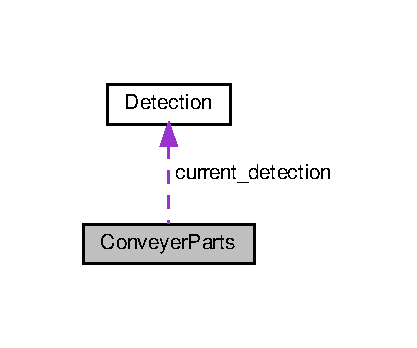
\includegraphics[width=200pt]{classConveyerParts__coll__graph}
\end{center}
\end{figure}
\subsection*{Public Member Functions}
\begin{DoxyCompactItemize}
\item 
void \hyperlink{classConveyerParts_a4e63b43cf4de0e31ed58a89b1fc2654c}{conveyer\+Logical\+Camera\+Callback} (const nist\+\_\+gear\+::\+Logical\+Camera\+Image \&msg)
\begin{DoxyCompactList}\small\item\em Conveyor logical camera callback. \end{DoxyCompactList}\item 
\hyperlink{classConveyerParts_a0b511cdd3b2d0c0587901b1443f43d49}{Conveyer\+Parts} (ros\+::\+Node\+Handle \&node)
\begin{DoxyCompactList}\small\item\em Constructor. \end{DoxyCompactList}\item 
void \hyperlink{classConveyerParts_ab701aac222b631fdf7a1d2a3465eaa67}{Init} ()
\begin{DoxyCompactList}\small\item\em Initialization. \end{DoxyCompactList}\item 
bool \hyperlink{classConveyerParts_aaa9a8364efc6d4247d8d5585b6b21859}{check\+Part} (const std\+::string \&part\+\_\+name)
\begin{DoxyCompactList}\small\item\em Checks for part. \end{DoxyCompactList}\item 
bool \hyperlink{classConveyerParts_a57188292039617070e9042ad3133a5f8}{give\+Closest\+Part} (const std\+::string \&part\+\_\+name, geometry\+\_\+msgs\+::\+Pose \&pose\+On\+Conveyer)
\begin{DoxyCompactList}\small\item\em Gets closest part. \end{DoxyCompactList}\item 
bool \hyperlink{classConveyerParts_a8a536ff479f28fcb38cf454a41f8387e}{check\+For\+Pick} ()
\begin{DoxyCompactList}\small\item\em Checks if part ready to pickup. \end{DoxyCompactList}\end{DoxyCompactItemize}
\subsection*{Public Attributes}
\begin{DoxyCompactItemize}
\item 
\mbox{\Hypertarget{classConveyerParts_a8cd52489a957397b51b4e1be2bcd84d9}\label{classConveyerParts_a8cd52489a957397b51b4e1be2bcd84d9}} 
ros\+::\+Subscriber \hyperlink{classConveyerParts_a8cd52489a957397b51b4e1be2bcd84d9}{conveyer\+\_\+subscriber}
\begin{DoxyCompactList}\small\item\em Conveyer subscriber variable. \end{DoxyCompactList}\item 
\mbox{\Hypertarget{classConveyerParts_aa604a79b48159e651800911a4c26a13d}\label{classConveyerParts_aa604a79b48159e651800911a4c26a13d}} 
\hyperlink{classDetection}{Detection} \hyperlink{classConveyerParts_aa604a79b48159e651800911a4c26a13d}{current\+\_\+detection}
\begin{DoxyCompactList}\small\item\em Current detection variable. \end{DoxyCompactList}\item 
std\+::vector$<$ \hyperlink{classDetection}{Detection} $>$ \hyperlink{classConveyerParts_ab75ade698ffee71ccf3792d22917eb95}{all\+Conveyer\+Parts}
\begin{DoxyCompactList}\small\item\em All Conveyer Parts variable. \end{DoxyCompactList}\item 
\mbox{\Hypertarget{classConveyerParts_a4147928a7d87b11ad6dfa179cbfc3a5c}\label{classConveyerParts_a4147928a7d87b11ad6dfa179cbfc3a5c}} 
double \hyperlink{classConveyerParts_a4147928a7d87b11ad6dfa179cbfc3a5c}{estimated\+\_\+time} =0
\begin{DoxyCompactList}\small\item\em Estimated time. \end{DoxyCompactList}\end{DoxyCompactItemize}


\subsection{Detailed Description}
Conveyor parts class. 

\subsection{Constructor \& Destructor Documentation}
\mbox{\Hypertarget{classConveyerParts_a0b511cdd3b2d0c0587901b1443f43d49}\label{classConveyerParts_a0b511cdd3b2d0c0587901b1443f43d49}} 
\index{Conveyer\+Parts@{Conveyer\+Parts}!Conveyer\+Parts@{Conveyer\+Parts}}
\index{Conveyer\+Parts@{Conveyer\+Parts}!Conveyer\+Parts@{Conveyer\+Parts}}
\subsubsection{\texorpdfstring{Conveyer\+Parts()}{ConveyerParts()}}
{\footnotesize\ttfamily Conveyer\+Parts\+::\+Conveyer\+Parts (\begin{DoxyParamCaption}\item[{ros\+::\+Node\+Handle \&}]{node }\end{DoxyParamCaption})}



Constructor. 


\begin{DoxyParams}{Parameters}
{\em node} & R\+OS nodehandle \\
\hline
\end{DoxyParams}
\begin{DoxyReturn}{Returns}
None 
\end{DoxyReturn}


\subsection{Member Function Documentation}
\mbox{\Hypertarget{classConveyerParts_a8a536ff479f28fcb38cf454a41f8387e}\label{classConveyerParts_a8a536ff479f28fcb38cf454a41f8387e}} 
\index{Conveyer\+Parts@{Conveyer\+Parts}!check\+For\+Pick@{check\+For\+Pick}}
\index{check\+For\+Pick@{check\+For\+Pick}!Conveyer\+Parts@{Conveyer\+Parts}}
\subsubsection{\texorpdfstring{check\+For\+Pick()}{checkForPick()}}
{\footnotesize\ttfamily bool Conveyer\+Parts\+::check\+For\+Pick (\begin{DoxyParamCaption}{ }\end{DoxyParamCaption})}



Checks if part ready to pickup. 


\begin{DoxyParams}{Parameters}
{\em None} & \\
\hline
\end{DoxyParams}
\begin{DoxyReturn}{Returns}
True if ready to be picked up else false 
\end{DoxyReturn}
\mbox{\Hypertarget{classConveyerParts_aaa9a8364efc6d4247d8d5585b6b21859}\label{classConveyerParts_aaa9a8364efc6d4247d8d5585b6b21859}} 
\index{Conveyer\+Parts@{Conveyer\+Parts}!check\+Part@{check\+Part}}
\index{check\+Part@{check\+Part}!Conveyer\+Parts@{Conveyer\+Parts}}
\subsubsection{\texorpdfstring{check\+Part()}{checkPart()}}
{\footnotesize\ttfamily bool Conveyer\+Parts\+::check\+Part (\begin{DoxyParamCaption}\item[{const std\+::string \&}]{part\+\_\+name }\end{DoxyParamCaption})}



Checks for part. 


\begin{DoxyParams}{Parameters}
{\em part\+\_\+name} & \hyperlink{structPart}{Part} name \\
\hline
\end{DoxyParams}
\begin{DoxyReturn}{Returns}
None 
\end{DoxyReturn}
\mbox{\Hypertarget{classConveyerParts_a4e63b43cf4de0e31ed58a89b1fc2654c}\label{classConveyerParts_a4e63b43cf4de0e31ed58a89b1fc2654c}} 
\index{Conveyer\+Parts@{Conveyer\+Parts}!conveyer\+Logical\+Camera\+Callback@{conveyer\+Logical\+Camera\+Callback}}
\index{conveyer\+Logical\+Camera\+Callback@{conveyer\+Logical\+Camera\+Callback}!Conveyer\+Parts@{Conveyer\+Parts}}
\subsubsection{\texorpdfstring{conveyer\+Logical\+Camera\+Callback()}{conveyerLogicalCameraCallback()}}
{\footnotesize\ttfamily void Conveyer\+Parts\+::conveyer\+Logical\+Camera\+Callback (\begin{DoxyParamCaption}\item[{const nist\+\_\+gear\+::\+Logical\+Camera\+Image \&}]{msg }\end{DoxyParamCaption})}



Conveyor logical camera callback. 


\begin{DoxyParams}{Parameters}
{\em msg} & Logical camera image \\
\hline
\end{DoxyParams}
\begin{DoxyReturn}{Returns}
None 
\end{DoxyReturn}
\mbox{\Hypertarget{classConveyerParts_a57188292039617070e9042ad3133a5f8}\label{classConveyerParts_a57188292039617070e9042ad3133a5f8}} 
\index{Conveyer\+Parts@{Conveyer\+Parts}!give\+Closest\+Part@{give\+Closest\+Part}}
\index{give\+Closest\+Part@{give\+Closest\+Part}!Conveyer\+Parts@{Conveyer\+Parts}}
\subsubsection{\texorpdfstring{give\+Closest\+Part()}{giveClosestPart()}}
{\footnotesize\ttfamily bool Conveyer\+Parts\+::give\+Closest\+Part (\begin{DoxyParamCaption}\item[{const std\+::string \&}]{part\+\_\+name,  }\item[{geometry\+\_\+msgs\+::\+Pose \&}]{pose\+On\+Conveyer }\end{DoxyParamCaption})}



Gets closest part. 


\begin{DoxyParams}{Parameters}
{\em part\+\_\+name} & \hyperlink{structPart}{Part} name \\
\hline
{\em pose\+On\+Conveyer} & Current pose of part on conveyor \\
\hline
\end{DoxyParams}
\begin{DoxyReturn}{Returns}
True/\+False 
\end{DoxyReturn}
\mbox{\Hypertarget{classConveyerParts_ab701aac222b631fdf7a1d2a3465eaa67}\label{classConveyerParts_ab701aac222b631fdf7a1d2a3465eaa67}} 
\index{Conveyer\+Parts@{Conveyer\+Parts}!Init@{Init}}
\index{Init@{Init}!Conveyer\+Parts@{Conveyer\+Parts}}
\subsubsection{\texorpdfstring{Init()}{Init()}}
{\footnotesize\ttfamily void Conveyer\+Parts\+::\+Init (\begin{DoxyParamCaption}{ }\end{DoxyParamCaption})}



Initialization. 


\begin{DoxyParams}{Parameters}
{\em None} & \\
\hline
\end{DoxyParams}
\begin{DoxyReturn}{Returns}
None 
\end{DoxyReturn}


\subsection{Member Data Documentation}
\mbox{\Hypertarget{classConveyerParts_ab75ade698ffee71ccf3792d22917eb95}\label{classConveyerParts_ab75ade698ffee71ccf3792d22917eb95}} 
\index{Conveyer\+Parts@{Conveyer\+Parts}!all\+Conveyer\+Parts@{all\+Conveyer\+Parts}}
\index{all\+Conveyer\+Parts@{all\+Conveyer\+Parts}!Conveyer\+Parts@{Conveyer\+Parts}}
\subsubsection{\texorpdfstring{all\+Conveyer\+Parts}{allConveyerParts}}
{\footnotesize\ttfamily std\+::vector$<$\hyperlink{classDetection}{Detection}$>$ Conveyer\+Parts\+::all\+Conveyer\+Parts}



All Conveyer Parts variable. 


\begin{DoxyParams}{Parameters}
{\em None} & \\
\hline
\end{DoxyParams}
\begin{DoxyReturn}{Returns}
None 
\end{DoxyReturn}


The documentation for this class was generated from the following files\+:\begin{DoxyCompactItemize}
\item 
include/conveyer.\+h\item 
src/conveyer.\+cpp\end{DoxyCompactItemize}

\hypertarget{classDetection}{}\section{Detection Class Reference}
\label{classDetection}\index{Detection@{Detection}}


\hyperlink{classDetection}{Detection} class.  




{\ttfamily \#include $<$conveyer.\+h$>$}

\subsection*{Public Member Functions}
\begin{DoxyCompactItemize}
\item 
void \hyperlink{classDetection_ab9da7e3347faeced1a83edbdbb9843ee}{empty\+Detection} ()
\begin{DoxyCompactList}\small\item\em Resets detection parameters. \end{DoxyCompactList}\end{DoxyCompactItemize}
\subsection*{Public Attributes}
\begin{DoxyCompactItemize}
\item 
\mbox{\Hypertarget{classDetection_acb409f4e2a2d962adbf1380f0af3cd91}\label{classDetection_acb409f4e2a2d962adbf1380f0af3cd91}} 
bool \hyperlink{classDetection_acb409f4e2a2d962adbf1380f0af3cd91}{part\+\_\+set} = false
\begin{DoxyCompactList}\small\item\em \hyperlink{structPart}{Part} set variable. \end{DoxyCompactList}\item 
\mbox{\Hypertarget{classDetection_ac65c8965d50a3ed3e89c4331b48bd0fe}\label{classDetection_ac65c8965d50a3ed3e89c4331b48bd0fe}} 
bool \hyperlink{classDetection_ac65c8965d50a3ed3e89c4331b48bd0fe}{picked\+\_\+up} = false
\begin{DoxyCompactList}\small\item\em Picked up variable. \end{DoxyCompactList}\item 
\mbox{\Hypertarget{classDetection_a5c059835a0756f2a37013aab11dd1648}\label{classDetection_a5c059835a0756f2a37013aab11dd1648}} 
double \hyperlink{classDetection_a5c059835a0756f2a37013aab11dd1648}{first\+\_\+look\+\_\+time} =-\/1
\begin{DoxyCompactList}\small\item\em First look time variable. \end{DoxyCompactList}\item 
\mbox{\Hypertarget{classDetection_a9765464cc571b70ed841bdf0f5384a9d}\label{classDetection_a9765464cc571b70ed841bdf0f5384a9d}} 
double \hyperlink{classDetection_a9765464cc571b70ed841bdf0f5384a9d}{second\+\_\+look\+\_\+time} =-\/1
\begin{DoxyCompactList}\small\item\em Second look time variable. \end{DoxyCompactList}\item 
\mbox{\Hypertarget{classDetection_a4764e067ed7cbeda827c34fcc0dc40b5}\label{classDetection_a4764e067ed7cbeda827c34fcc0dc40b5}} 
double \hyperlink{classDetection_a4764e067ed7cbeda827c34fcc0dc40b5}{speed} =-\/1
\begin{DoxyCompactList}\small\item\em Speed variable. \end{DoxyCompactList}\item 
\mbox{\Hypertarget{classDetection_a4ab4e17edde2c524b27b6c0a7cd553a3}\label{classDetection_a4ab4e17edde2c524b27b6c0a7cd553a3}} 
std\+::string \hyperlink{classDetection_a4ab4e17edde2c524b27b6c0a7cd553a3}{type} =\char`\"{}\char`\"{}
\begin{DoxyCompactList}\small\item\em Type variable. \end{DoxyCompactList}\item 
\mbox{\Hypertarget{classDetection_aa81dc0bbc383403eca0a313d7fb38d47}\label{classDetection_aa81dc0bbc383403eca0a313d7fb38d47}} 
geometry\+\_\+msgs\+::\+Pose \hyperlink{classDetection_aa81dc0bbc383403eca0a313d7fb38d47}{first\+\_\+pose}
\begin{DoxyCompactList}\small\item\em Pose 1 variable. \end{DoxyCompactList}\item 
\mbox{\Hypertarget{classDetection_a0a0e90d58cd33f97d243fb439b201dcd}\label{classDetection_a0a0e90d58cd33f97d243fb439b201dcd}} 
geometry\+\_\+msgs\+::\+Pose \hyperlink{classDetection_a0a0e90d58cd33f97d243fb439b201dcd}{second\+\_\+pose}
\begin{DoxyCompactList}\small\item\em Pose 2 variable. \end{DoxyCompactList}\item 
\mbox{\Hypertarget{classDetection_ab5c9ff6b31a682762262b930e5fb8de1}\label{classDetection_ab5c9ff6b31a682762262b930e5fb8de1}} 
geometry\+\_\+msgs\+::\+Pose \hyperlink{classDetection_ab5c9ff6b31a682762262b930e5fb8de1}{current\+\_\+pose}
\begin{DoxyCompactList}\small\item\em Current pose variable. \end{DoxyCompactList}\end{DoxyCompactItemize}


\subsection{Detailed Description}
\hyperlink{classDetection}{Detection} class. 

\subsection{Member Function Documentation}
\mbox{\Hypertarget{classDetection_ab9da7e3347faeced1a83edbdbb9843ee}\label{classDetection_ab9da7e3347faeced1a83edbdbb9843ee}} 
\index{Detection@{Detection}!empty\+Detection@{empty\+Detection}}
\index{empty\+Detection@{empty\+Detection}!Detection@{Detection}}
\subsubsection{\texorpdfstring{empty\+Detection()}{emptyDetection()}}
{\footnotesize\ttfamily void Detection\+::empty\+Detection (\begin{DoxyParamCaption}{ }\end{DoxyParamCaption})}



Resets detection parameters. 


\begin{DoxyParams}{Parameters}
{\em None} & \\
\hline
\end{DoxyParams}
\begin{DoxyReturn}{Returns}
None 
\end{DoxyReturn}


The documentation for this class was generated from the following files\+:\begin{DoxyCompactItemize}
\item 
include/conveyer.\+h\item 
src/conveyer.\+cpp\end{DoxyCompactItemize}

\hypertarget{classGantryControl}{}\section{Gantry\+Control Class Reference}
\label{classGantryControl}\index{Gantry\+Control@{Gantry\+Control}}


Gantry Control class.  




{\ttfamily \#include $<$gantry\+\_\+control.\+h$>$}



Collaboration diagram for Gantry\+Control\+:\nopagebreak
\begin{figure}[H]
\begin{center}
\leavevmode
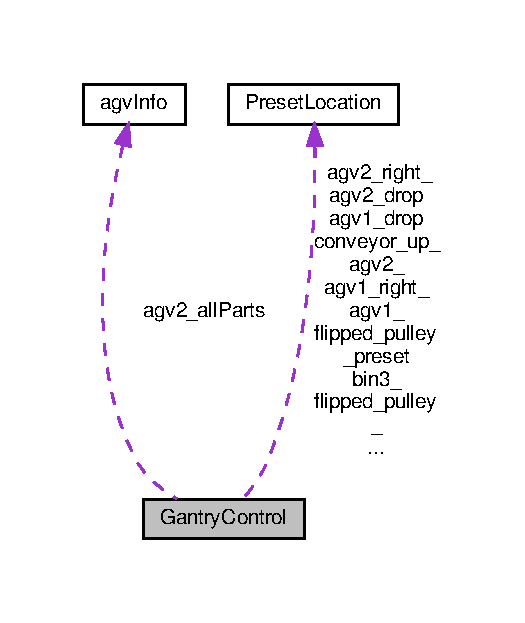
\includegraphics[width=252pt]{classGantryControl__coll__graph}
\end{center}
\end{figure}
\subsection*{Public Member Functions}
\begin{DoxyCompactItemize}
\item 
\hyperlink{classGantryControl_a9b8ad2f8dda14130976eb5d9634acbae}{Gantry\+Control} (ros\+::\+Node\+Handle \&node)
\begin{DoxyCompactList}\small\item\em Constructor. \end{DoxyCompactList}\item 
void \hyperlink{classGantryControl_a71f13d325c732d931ed5ed175c5b3e7a}{init} ()
\begin{DoxyCompactList}\small\item\em Initialization. \end{DoxyCompactList}\item 
\hyperlink{utils_8h_abd807f196b951c0cdd24d50164d54763}{stats} \hyperlink{classGantryControl_a2ac175070ddb578c03bb5a33cf2d49a4}{get\+Stats} (std\+::string function)
\begin{DoxyCompactList}\small\item\em Gets the stats. \end{DoxyCompactList}\item 
void \hyperlink{classGantryControl_a6557b18bde7b776e6a05fe85d9e858d9}{quality\+Callback1} (const nist\+\_\+gear\+::\+Logical\+Camera\+Image \&msg)
\begin{DoxyCompactList}\small\item\em Quality camera 1 callback. \end{DoxyCompactList}\item 
void \hyperlink{classGantryControl_a355b299969bfa74073062ba1c6c1ec04}{quality\+Callback2} (const nist\+\_\+gear\+::\+Logical\+Camera\+Image \&msg)
\begin{DoxyCompactList}\small\item\em Quality camera 2 callback. \end{DoxyCompactList}\item 
bool \hyperlink{classGantryControl_af9280bbee71d1ceca8aef3d616d48254}{pick\+Part} (\hyperlink{utils_8h_a67ee3a5b9091664130eca8efc8b97ab9}{part} \hyperlink{utils_8h_a67ee3a5b9091664130eca8efc8b97ab9}{part})
\begin{DoxyCompactList}\small\item\em Makes robot pick the part. \end{DoxyCompactList}\item 
bool \hyperlink{classGantryControl_a0d0eb41f65891a98cae6f2a4a42d281a}{place\+Part} (\hyperlink{utils_8h_a48a7207852c0455cce7e65703b12ec7e}{product} \&\hyperlink{utils_8h_a48a7207852c0455cce7e65703b12ec7e}{product}, std\+::string agv, std\+::string arm)
\begin{DoxyCompactList}\small\item\em Makes robot place the part. \end{DoxyCompactList}\item 
bool \hyperlink{classGantryControl_ab271ce06b0d336eddb26e1ba5a2ce594}{send\+\_\+command} (trajectory\+\_\+msgs\+::\+Joint\+Trajectory command\+\_\+msg)
\begin{DoxyCompactList}\small\item\em Send command message to robot controller. \end{DoxyCompactList}\item 
void \hyperlink{classGantryControl_a6986d4f622840037e003c6db840d78ed}{go\+To\+Preset\+Location} (\hyperlink{structPresetLocation}{Preset\+Location} location)
\begin{DoxyCompactList}\small\item\em Makes robot move to preset location. \end{DoxyCompactList}\item 
void \hyperlink{classGantryControl_ad7a304b37a95f29634631d4183276be3}{rotate\+\_\+gantry} (double angle)
\begin{DoxyCompactList}\small\item\em Rotate gantry. \end{DoxyCompactList}\item 
void \hyperlink{classGantryControl_aaccd9c43b5564c198288ba51cbcecabe}{activate\+Gripper} (std\+::string gripper\+\_\+id)
\begin{DoxyCompactList}\small\item\em Activate gripper. \end{DoxyCompactList}\item 
void \hyperlink{classGantryControl_a1485577d4e29baf708a4c5c028a47798}{deactivate\+Gripper} (std\+::string gripper\+\_\+id)
\begin{DoxyCompactList}\small\item\em deactivate\+Gripper \end{DoxyCompactList}\item 
void \hyperlink{classGantryControl_a9206feae49953cf691e0dec2331cc3ae}{logical\+Callback16} (const nist\+\_\+gear\+::\+Logical\+Camera\+Image \&msg)
\begin{DoxyCompactList}\small\item\em Logical camera 16 callback. \end{DoxyCompactList}\item 
void \hyperlink{classGantryControl_a9d745504ec1dbcc8549f5a604f34bbcc}{logical\+Callback17} (const nist\+\_\+gear\+::\+Logical\+Camera\+Image \&msg)
\begin{DoxyCompactList}\small\item\em Logical camera 17 callback. \end{DoxyCompactList}\item 
void \hyperlink{classGantryControl_a0220eeac3687f7f043fa4014f5ea302e}{pick\+From\+Conveyor} (\hyperlink{structProduct}{Product} \&\hyperlink{utils_8h_a48a7207852c0455cce7e65703b12ec7e}{product}, \hyperlink{classConveyerParts}{Conveyer\+Parts} \&conveyer\+Parts\+Obj)
\begin{DoxyCompactList}\small\item\em Pick from conveyor. \end{DoxyCompactList}\item 
bool \hyperlink{classGantryControl_a9c655daed586e64921ffc53cb90b2873}{pose\+Matches} (const geometry\+\_\+msgs\+::\+Pose \&pose1, const geometry\+\_\+msgs\+::\+Pose \&pose2)
\begin{DoxyCompactList}\small\item\em Pose Matches. \end{DoxyCompactList}\item 
bool \hyperlink{classGantryControl_a31672ce076ba59662af6c77c82ab136f}{check\+\_\+exist\+\_\+on\+\_\+agv} (const std\+::string \&name, const geometry\+\_\+msgs\+::\+Pose \&part\+\_\+pose, \hyperlink{structagvInfo}{agv\+Info} \&agv)
\begin{DoxyCompactList}\small\item\em Check if a part exists on A\+GV. \end{DoxyCompactList}\item 
void \hyperlink{classGantryControl_a80a0b29105892d6435ef1bb061f35d8f}{flip\+Part} ()
\begin{DoxyCompactList}\small\item\em Flip part. \end{DoxyCompactList}\item 
bool \hyperlink{classGantryControl_adfbb542c0c4b836ec50bc7cf70557220}{move2start} (float x, float y, std\+::vector$<$ double $>$ left\+\_\+arm)
\begin{DoxyCompactList}\small\item\em Moves robot to start position. \end{DoxyCompactList}\item 
std\+::vector$<$ double $>$ \hyperlink{classGantryControl_aa3b48219dcba01f5608c6a4d9ff447e9}{move2trg} (float x, float y, float \&gantryX, float \&gantryY, int curr\+Gap, std\+::vector$<$ double $>$ left\+\_\+arm)
\begin{DoxyCompactList}\small\item\em Move to target. \end{DoxyCompactList}\item 
bool \hyperlink{classGantryControl_aa6ba7baf102ac7e39d68b2ae2492f9a5}{move2closest\+Gap} (struct \hyperlink{structPart}{Part} \&\hyperlink{utils_8h_a67ee3a5b9091664130eca8efc8b97ab9}{part}, std\+::vector$<$ std\+::pair$<$ float, float $>$ $>$ \&shelf\+Gaps, const std\+::vector$<$ int $>$ \&gap\+Num, bool act\+Part, float \&gantryX, float \&gantryY, \hyperlink{classObstaclesInAisle}{Obstacles\+In\+Aisle} \&obj, int \&new\+Gap)
\begin{DoxyCompactList}\small\item\em Move to closest gap. \end{DoxyCompactList}\item 
int \hyperlink{classGantryControl_ab475e912ab1ea0d13efc10078695102e}{get\+Nearest\+Gap} (float destX, int aisle\+\_\+num, bool act\+Part, \hyperlink{classObstaclesInAisle}{Obstacles\+In\+Aisle} \&obst\+Obj, const std\+::vector$<$ std\+::pair$<$ float, float $>$ $>$ \&shelf\+Gaps)
\begin{DoxyCompactList}\small\item\em Gets the nearest gap from shelf. \end{DoxyCompactList}\item 
bool \hyperlink{classGantryControl_aa014dd433af4fc580d38639c6353e7b8}{escape} (int \&aisle\+\_\+num, std\+::vector$<$ std\+::pair$<$ float, float $>$ $>$ \&shelf\+Gaps, const std\+::vector$<$ int $>$ \&gap\+Num, bool act\+Part, float \&gantryX, float \&gantryY, \hyperlink{classObstaclesInAisle}{Obstacles\+In\+Aisle} \&obst\+Obj, int \&new\+Gap, std\+::vector$<$ double $>$ \&left\+\_\+arm, bool pick\+Status)
\begin{DoxyCompactList}\small\item\em Makes robot escape from Aisle. \end{DoxyCompactList}\item 
geometry\+\_\+msgs\+::\+Pose \hyperlink{classGantryControl_aefa12231efd7960bc201638f832d9478}{get\+Robot\+Pose} ()
\begin{DoxyCompactList}\small\item\em Gets the robot pose. \end{DoxyCompactList}\item 
nist\+\_\+gear\+::\+Vacuum\+Gripper\+State \hyperlink{classGantryControl_a986691834604135cf47b1c070f8d915e}{get\+Gripper\+State} (std\+::string arm\+\_\+name)
\begin{DoxyCompactList}\small\item\em Gets the gripper state. \end{DoxyCompactList}\item 
geometry\+\_\+msgs\+::\+Pose \hyperlink{classGantryControl_ae92c2fdeba302399425c1abafc76f973}{get\+Target\+World\+Pose} (geometry\+\_\+msgs\+::\+Pose target, std\+::string agv, std\+::string arm)
\begin{DoxyCompactList}\small\item\em Gets target pose in world frame. \end{DoxyCompactList}\end{DoxyCompactItemize}
\subsection*{Public Attributes}
\begin{DoxyCompactItemize}
\item 
\mbox{\Hypertarget{classGantryControl_a34ef8dd7ccc4b5bca673caca267b8cae}\label{classGantryControl_a34ef8dd7ccc4b5bca673caca267b8cae}} 
int \hyperlink{classGantryControl_a34ef8dd7ccc4b5bca673caca267b8cae}{quality\+\_\+call\+\_\+count} =0
\begin{DoxyCompactList}\small\item\em Quality call count variable. \end{DoxyCompactList}\item 
\mbox{\Hypertarget{classGantryControl_a5a45b3fc19e50496208af90d8c49590d}\label{classGantryControl_a5a45b3fc19e50496208af90d8c49590d}} 
\hyperlink{utils_8h_a36494ad089a17d7ae00c4cc799ed0970}{start} \hyperlink{classGantryControl_a5a45b3fc19e50496208af90d8c49590d}{start\+\_\+}
\begin{DoxyCompactList}\small\item\em Start preset location. \end{DoxyCompactList}\item 
\mbox{\Hypertarget{classGantryControl_a50911044f2a712e70d35ad0513a1d3cf}\label{classGantryControl_a50911044f2a712e70d35ad0513a1d3cf}} 
\hyperlink{structPresetLocation}{bin3} \hyperlink{classGantryControl_a50911044f2a712e70d35ad0513a1d3cf}{bin3\+\_\+}
\begin{DoxyCompactList}\small\item\em Bin 3 preset location. \end{DoxyCompactList}\item 
\mbox{\Hypertarget{classGantryControl_aafaf6e121f9340813966dc81aaf0853f}\label{classGantryControl_aafaf6e121f9340813966dc81aaf0853f}} 
\hyperlink{structPresetLocation}{flipped\+\_\+pulley} \hyperlink{classGantryControl_aafaf6e121f9340813966dc81aaf0853f}{flipped\+\_\+pulley\+\_\+}
\begin{DoxyCompactList}\small\item\em Flipped pulley \& Flipped pulley Preset location. \end{DoxyCompactList}\item 
\mbox{\Hypertarget{classGantryControl_addcefc6d7411cbb92b007eb21afc6cd1}\label{classGantryControl_addcefc6d7411cbb92b007eb21afc6cd1}} 
\hyperlink{structPresetLocation}{flipped\+\_\+pulley} {\bfseries flipped\+\_\+pulley\+\_\+preset}
\item 
\mbox{\Hypertarget{classGantryControl_acf9dbf2d68e9cc06a5ac71f88f1f313d}\label{classGantryControl_acf9dbf2d68e9cc06a5ac71f88f1f313d}} 
\hyperlink{structPresetLocation}{agv1} \hyperlink{classGantryControl_acf9dbf2d68e9cc06a5ac71f88f1f313d}{agv1\+\_\+}
\begin{DoxyCompactList}\small\item\em A\+G\+V1 Preset Locations. \end{DoxyCompactList}\item 
\mbox{\Hypertarget{classGantryControl_a9b61b6968325f0f602d3a0db40634ddb}\label{classGantryControl_a9b61b6968325f0f602d3a0db40634ddb}} 
\hyperlink{structPresetLocation}{agv1} {\bfseries agv1\+\_\+drop}
\item 
\mbox{\Hypertarget{classGantryControl_a34e2582f1799acde6587eafb805aa36a}\label{classGantryControl_a34e2582f1799acde6587eafb805aa36a}} 
\hyperlink{structPresetLocation}{agv1} {\bfseries agv1\+\_\+right\+\_\+}
\item 
\mbox{\Hypertarget{classGantryControl_ac7b1c37af6a9ccce853e821b36088c42}\label{classGantryControl_ac7b1c37af6a9ccce853e821b36088c42}} 
\hyperlink{structPresetLocation}{agv2} \hyperlink{classGantryControl_ac7b1c37af6a9ccce853e821b36088c42}{agv2\+\_\+}
\begin{DoxyCompactList}\small\item\em A\+G\+V2 Preset Locations. \end{DoxyCompactList}\item 
\mbox{\Hypertarget{classGantryControl_abc7a7f96e8ba220e0c95e1ab8292e200}\label{classGantryControl_abc7a7f96e8ba220e0c95e1ab8292e200}} 
\hyperlink{structPresetLocation}{agv2} {\bfseries agv2\+\_\+drop}
\item 
\mbox{\Hypertarget{classGantryControl_a0d329f5035a3f83d370713ef25431ff0}\label{classGantryControl_a0d329f5035a3f83d370713ef25431ff0}} 
\hyperlink{structPresetLocation}{agv2} {\bfseries agv2\+\_\+right\+\_\+}
\item 
\mbox{\Hypertarget{classGantryControl_a72d258b3cce201922919fc6a4105f09a}\label{classGantryControl_a72d258b3cce201922919fc6a4105f09a}} 
\hyperlink{structPresetLocation}{conveyor\+\_\+up} \hyperlink{classGantryControl_a72d258b3cce201922919fc6a4105f09a}{conveyor\+\_\+up\+\_\+}
\begin{DoxyCompactList}\small\item\em Conveyor up Preset location. \end{DoxyCompactList}\item 
\mbox{\Hypertarget{classGantryControl_a79ac55bacfc11034d9fdd83920b3871d}\label{classGantryControl_a79ac55bacfc11034d9fdd83920b3871d}} 
struct \hyperlink{structagvInfo}{agv\+Info} agv1\+\_\+all\+Parts \hyperlink{classGantryControl_a79ac55bacfc11034d9fdd83920b3871d}{agv2\+\_\+all\+Parts}
\begin{DoxyCompactList}\small\item\em A\+GV information. \end{DoxyCompactList}\item 
\mbox{\Hypertarget{classGantryControl_a568d5391ab16be3d57db4f48379dcaa6}\label{classGantryControl_a568d5391ab16be3d57db4f48379dcaa6}} 
bool \hyperlink{classGantryControl_a568d5391ab16be3d57db4f48379dcaa6}{agv1\+\_\+allocated} = false
\begin{DoxyCompactList}\small\item\em A\+G\+V1 allocated flag. \end{DoxyCompactList}\item 
\mbox{\Hypertarget{classGantryControl_afde665598b615a44b753bb2208d11afc}\label{classGantryControl_afde665598b615a44b753bb2208d11afc}} 
bool \hyperlink{classGantryControl_afde665598b615a44b753bb2208d11afc}{agv2\+\_\+allocated} = false
\begin{DoxyCompactList}\small\item\em A\+G\+V2 allocated flag. \end{DoxyCompactList}\end{DoxyCompactItemize}
\subsection*{Static Public Attributes}
\begin{DoxyCompactItemize}
\item 
\mbox{\Hypertarget{classGantryControl_abea9b6d47cfab1e5e6761206c5d32770}\label{classGantryControl_abea9b6d47cfab1e5e6761206c5d32770}} 
static const int \hyperlink{classGantryControl_abea9b6d47cfab1e5e6761206c5d32770}{num\+\_\+pre\+Loc} = 20
\begin{DoxyCompactList}\small\item\em Num pre\+Loc. \end{DoxyCompactList}\end{DoxyCompactItemize}


\subsection{Detailed Description}
Gantry Control class. 

\subsection{Constructor \& Destructor Documentation}
\mbox{\Hypertarget{classGantryControl_a9b8ad2f8dda14130976eb5d9634acbae}\label{classGantryControl_a9b8ad2f8dda14130976eb5d9634acbae}} 
\index{Gantry\+Control@{Gantry\+Control}!Gantry\+Control@{Gantry\+Control}}
\index{Gantry\+Control@{Gantry\+Control}!Gantry\+Control@{Gantry\+Control}}
\subsubsection{\texorpdfstring{Gantry\+Control()}{GantryControl()}}
{\footnotesize\ttfamily Gantry\+Control\+::\+Gantry\+Control (\begin{DoxyParamCaption}\item[{ros\+::\+Node\+Handle \&}]{node }\end{DoxyParamCaption})}



Constructor. 


\begin{DoxyParams}{Parameters}
{\em node} & R\+OS nodehandle \\
\hline
\end{DoxyParams}
\begin{DoxyReturn}{Returns}
None 
\end{DoxyReturn}


\subsection{Member Function Documentation}
\mbox{\Hypertarget{classGantryControl_aaccd9c43b5564c198288ba51cbcecabe}\label{classGantryControl_aaccd9c43b5564c198288ba51cbcecabe}} 
\index{Gantry\+Control@{Gantry\+Control}!activate\+Gripper@{activate\+Gripper}}
\index{activate\+Gripper@{activate\+Gripper}!Gantry\+Control@{Gantry\+Control}}
\subsubsection{\texorpdfstring{activate\+Gripper()}{activateGripper()}}
{\footnotesize\ttfamily void Gantry\+Control\+::activate\+Gripper (\begin{DoxyParamCaption}\item[{std\+::string}]{gripper\+\_\+id }\end{DoxyParamCaption})}



Activate gripper. 

Turn on vacuum gripper.


\begin{DoxyParams}{Parameters}
{\em gripper\+\_\+id} & Gripper ID \\
\hline
\end{DoxyParams}
\begin{DoxyReturn}{Returns}
None 
\end{DoxyReturn}
\mbox{\Hypertarget{classGantryControl_a31672ce076ba59662af6c77c82ab136f}\label{classGantryControl_a31672ce076ba59662af6c77c82ab136f}} 
\index{Gantry\+Control@{Gantry\+Control}!check\+\_\+exist\+\_\+on\+\_\+agv@{check\+\_\+exist\+\_\+on\+\_\+agv}}
\index{check\+\_\+exist\+\_\+on\+\_\+agv@{check\+\_\+exist\+\_\+on\+\_\+agv}!Gantry\+Control@{Gantry\+Control}}
\subsubsection{\texorpdfstring{check\+\_\+exist\+\_\+on\+\_\+agv()}{check\_exist\_on\_agv()}}
{\footnotesize\ttfamily bool Gantry\+Control\+::check\+\_\+exist\+\_\+on\+\_\+agv (\begin{DoxyParamCaption}\item[{const std\+::string \&}]{name,  }\item[{const geometry\+\_\+msgs\+::\+Pose \&}]{part\+\_\+pose,  }\item[{\hyperlink{structagvInfo}{agv\+Info} \&}]{agv }\end{DoxyParamCaption})}



Check if a part exists on A\+GV. 


\begin{DoxyParams}{Parameters}
{\em name} & Name \\
\hline
{\em part\+\_\+pose} & \hyperlink{structPart}{Part} pose \\
\hline
{\em agv} & A\+GV Info \\
\hline
\end{DoxyParams}
\begin{DoxyReturn}{Returns}
True if part exists on A\+GV else false 
\end{DoxyReturn}
\mbox{\Hypertarget{classGantryControl_a1485577d4e29baf708a4c5c028a47798}\label{classGantryControl_a1485577d4e29baf708a4c5c028a47798}} 
\index{Gantry\+Control@{Gantry\+Control}!deactivate\+Gripper@{deactivate\+Gripper}}
\index{deactivate\+Gripper@{deactivate\+Gripper}!Gantry\+Control@{Gantry\+Control}}
\subsubsection{\texorpdfstring{deactivate\+Gripper()}{deactivateGripper()}}
{\footnotesize\ttfamily void Gantry\+Control\+::deactivate\+Gripper (\begin{DoxyParamCaption}\item[{std\+::string}]{gripper\+\_\+id }\end{DoxyParamCaption})}



deactivate\+Gripper 

Turn off vacuum gripper.


\begin{DoxyParams}{Parameters}
{\em gripper\+\_\+id} & Gripper ID \\
\hline
\end{DoxyParams}
\begin{DoxyReturn}{Returns}
None 
\end{DoxyReturn}
\mbox{\Hypertarget{classGantryControl_aa014dd433af4fc580d38639c6353e7b8}\label{classGantryControl_aa014dd433af4fc580d38639c6353e7b8}} 
\index{Gantry\+Control@{Gantry\+Control}!escape@{escape}}
\index{escape@{escape}!Gantry\+Control@{Gantry\+Control}}
\subsubsection{\texorpdfstring{escape()}{escape()}}
{\footnotesize\ttfamily bool Gantry\+Control\+::escape (\begin{DoxyParamCaption}\item[{int \&}]{aisle\+\_\+num,  }\item[{std\+::vector$<$ std\+::pair$<$ float, float $>$ $>$ \&}]{shelf\+Gaps,  }\item[{const std\+::vector$<$ int $>$ \&}]{gap\+Num,  }\item[{bool}]{act\+Part,  }\item[{float \&}]{gantryX,  }\item[{float \&}]{gantryY,  }\item[{\hyperlink{classObstaclesInAisle}{Obstacles\+In\+Aisle} \&}]{obst\+Obj,  }\item[{int \&}]{new\+Gap,  }\item[{std\+::vector$<$ double $>$ \&}]{left\+\_\+arm,  }\item[{bool}]{pick\+Status }\end{DoxyParamCaption})}



Makes robot escape from Aisle. 


\begin{DoxyParams}{Parameters}
{\em aisle\+\_\+num} & Aisle number \\
\hline
{\em shelf\+Gaps} & Gap from shelves \\
\hline
{\em gap\+Num} & Gap number \\
\hline
{\em act\+Part} & Act part \\
\hline
{\em gantryX} & Gantry X-\/\+Coordinate \\
\hline
{\em gantryY} & Gantry Y-\/\+Coordinate \\
\hline
{\em obst\+Obj} & \hyperlink{classObstaclesInAisle}{Obstacles\+In\+Aisle} object \\
\hline
{\em new\+Gap} & Newgap from shelf \\
\hline
{\em left\+\_\+arm} & Left arm \\
\hline
{\em pick\+Status} & Status of pickup \\
\hline
\end{DoxyParams}
\begin{DoxyReturn}{Returns}
True if escape successfull else false 
\end{DoxyReturn}
\mbox{\Hypertarget{classGantryControl_a80a0b29105892d6435ef1bb061f35d8f}\label{classGantryControl_a80a0b29105892d6435ef1bb061f35d8f}} 
\index{Gantry\+Control@{Gantry\+Control}!flip\+Part@{flip\+Part}}
\index{flip\+Part@{flip\+Part}!Gantry\+Control@{Gantry\+Control}}
\subsubsection{\texorpdfstring{flip\+Part()}{flipPart()}}
{\footnotesize\ttfamily void Gantry\+Control\+::flip\+Part (\begin{DoxyParamCaption}{ }\end{DoxyParamCaption})}



Flip part. 


\begin{DoxyParams}{Parameters}
{\em None} & None \\
\hline
\end{DoxyParams}
\begin{DoxyReturn}{Returns}
None 
\end{DoxyReturn}
\mbox{\Hypertarget{classGantryControl_a986691834604135cf47b1c070f8d915e}\label{classGantryControl_a986691834604135cf47b1c070f8d915e}} 
\index{Gantry\+Control@{Gantry\+Control}!get\+Gripper\+State@{get\+Gripper\+State}}
\index{get\+Gripper\+State@{get\+Gripper\+State}!Gantry\+Control@{Gantry\+Control}}
\subsubsection{\texorpdfstring{get\+Gripper\+State()}{getGripperState()}}
{\footnotesize\ttfamily nist\+\_\+gear\+::\+Vacuum\+Gripper\+State Gantry\+Control\+::get\+Gripper\+State (\begin{DoxyParamCaption}\item[{std\+::string}]{arm\+\_\+name }\end{DoxyParamCaption})}



Gets the gripper state. 

Retrieve gripper state.


\begin{DoxyParams}{Parameters}
{\em arm\+\_\+name} & Arm name \\
\hline
\end{DoxyParams}
\begin{DoxyReturn}{Returns}
Gripper state 
\end{DoxyReturn}
\mbox{\Hypertarget{classGantryControl_ab475e912ab1ea0d13efc10078695102e}\label{classGantryControl_ab475e912ab1ea0d13efc10078695102e}} 
\index{Gantry\+Control@{Gantry\+Control}!get\+Nearest\+Gap@{get\+Nearest\+Gap}}
\index{get\+Nearest\+Gap@{get\+Nearest\+Gap}!Gantry\+Control@{Gantry\+Control}}
\subsubsection{\texorpdfstring{get\+Nearest\+Gap()}{getNearestGap()}}
{\footnotesize\ttfamily int Gantry\+Control\+::get\+Nearest\+Gap (\begin{DoxyParamCaption}\item[{float}]{destX,  }\item[{int}]{aisle\+\_\+num,  }\item[{bool}]{act\+Part,  }\item[{\hyperlink{classObstaclesInAisle}{Obstacles\+In\+Aisle} \&}]{obst\+Obj,  }\item[{const std\+::vector$<$ std\+::pair$<$ float, float $>$ $>$ \&}]{shelf\+Gaps }\end{DoxyParamCaption})}



Gets the nearest gap from shelf. 


\begin{DoxyParams}{Parameters}
{\em destX} & Destination X-\/\+Coordinate \\
\hline
{\em aisle\+\_\+num} & Aisle number \\
\hline
{\em act\+Part} & Act part \\
\hline
{\em obst\+Obj} & \hyperlink{classObstaclesInAisle}{Obstacles\+In\+Aisle} object \\
\hline
{\em shelf\+Gaps} & Gap from shelf \\
\hline
\end{DoxyParams}
\begin{DoxyReturn}{Returns}
Nearest gap from shelf 
\end{DoxyReturn}
\mbox{\Hypertarget{classGantryControl_aefa12231efd7960bc201638f832d9478}\label{classGantryControl_aefa12231efd7960bc201638f832d9478}} 
\index{Gantry\+Control@{Gantry\+Control}!get\+Robot\+Pose@{get\+Robot\+Pose}}
\index{get\+Robot\+Pose@{get\+Robot\+Pose}!Gantry\+Control@{Gantry\+Control}}
\subsubsection{\texorpdfstring{get\+Robot\+Pose()}{getRobotPose()}}
{\footnotesize\ttfamily geometry\+\_\+msgs\+::\+Pose Gantry\+Control\+::get\+Robot\+Pose (\begin{DoxyParamCaption}{ }\end{DoxyParamCaption})\hspace{0.3cm}{\ttfamily [inline]}}



Gets the robot pose. 


\begin{DoxyParams}{Parameters}
{\em None} & None \\
\hline
\end{DoxyParams}
\begin{DoxyReturn}{Returns}
Robot pose 
\end{DoxyReturn}
\mbox{\Hypertarget{classGantryControl_a2ac175070ddb578c03bb5a33cf2d49a4}\label{classGantryControl_a2ac175070ddb578c03bb5a33cf2d49a4}} 
\index{Gantry\+Control@{Gantry\+Control}!get\+Stats@{get\+Stats}}
\index{get\+Stats@{get\+Stats}!Gantry\+Control@{Gantry\+Control}}
\subsubsection{\texorpdfstring{get\+Stats()}{getStats()}}
{\footnotesize\ttfamily \hyperlink{utils_8h_abd807f196b951c0cdd24d50164d54763}{stats} Gantry\+Control\+::get\+Stats (\begin{DoxyParamCaption}\item[{std\+::string}]{function }\end{DoxyParamCaption})}



Gets the stats. 


\begin{DoxyParams}{Parameters}
{\em function} & Function \\
\hline
\end{DoxyParams}
\begin{DoxyReturn}{Returns}
\hyperlink{structStats}{Stats} 
\end{DoxyReturn}
\mbox{\Hypertarget{classGantryControl_ae92c2fdeba302399425c1abafc76f973}\label{classGantryControl_ae92c2fdeba302399425c1abafc76f973}} 
\index{Gantry\+Control@{Gantry\+Control}!get\+Target\+World\+Pose@{get\+Target\+World\+Pose}}
\index{get\+Target\+World\+Pose@{get\+Target\+World\+Pose}!Gantry\+Control@{Gantry\+Control}}
\subsubsection{\texorpdfstring{get\+Target\+World\+Pose()}{getTargetWorldPose()}}
{\footnotesize\ttfamily geometry\+\_\+msgs\+::\+Pose Gantry\+Control\+::get\+Target\+World\+Pose (\begin{DoxyParamCaption}\item[{geometry\+\_\+msgs\+::\+Pose}]{target,  }\item[{std\+::string}]{agv,  }\item[{std\+::string}]{arm }\end{DoxyParamCaption})}



Gets target pose in world frame. 


\begin{DoxyParams}{Parameters}
{\em target} & Target \\
\hline
{\em agv} & A\+GV Number \\
\hline
{\em arm} & Left/\+Right arm \\
\hline
\end{DoxyParams}
\begin{DoxyReturn}{Returns}
Target pose in world frame 
\end{DoxyReturn}
\mbox{\Hypertarget{classGantryControl_a6986d4f622840037e003c6db840d78ed}\label{classGantryControl_a6986d4f622840037e003c6db840d78ed}} 
\index{Gantry\+Control@{Gantry\+Control}!go\+To\+Preset\+Location@{go\+To\+Preset\+Location}}
\index{go\+To\+Preset\+Location@{go\+To\+Preset\+Location}!Gantry\+Control@{Gantry\+Control}}
\subsubsection{\texorpdfstring{go\+To\+Preset\+Location()}{goToPresetLocation()}}
{\footnotesize\ttfamily void Gantry\+Control\+::go\+To\+Preset\+Location (\begin{DoxyParamCaption}\item[{\hyperlink{structPresetLocation}{Preset\+Location}}]{location }\end{DoxyParamCaption})}



Makes robot move to preset location. 


\begin{DoxyParams}{Parameters}
{\em location} & Preset location \\
\hline
\end{DoxyParams}
\begin{DoxyReturn}{Returns}
None 
\end{DoxyReturn}
\mbox{\Hypertarget{classGantryControl_a71f13d325c732d931ed5ed175c5b3e7a}\label{classGantryControl_a71f13d325c732d931ed5ed175c5b3e7a}} 
\index{Gantry\+Control@{Gantry\+Control}!init@{init}}
\index{init@{init}!Gantry\+Control@{Gantry\+Control}}
\subsubsection{\texorpdfstring{init()}{init()}}
{\footnotesize\ttfamily void Gantry\+Control\+::init (\begin{DoxyParamCaption}{ }\end{DoxyParamCaption})}



Initialization. 


\begin{DoxyParams}{Parameters}
{\em None} & \\
\hline
\end{DoxyParams}
\begin{DoxyReturn}{Returns}
None 
\end{DoxyReturn}
\mbox{\Hypertarget{classGantryControl_a9206feae49953cf691e0dec2331cc3ae}\label{classGantryControl_a9206feae49953cf691e0dec2331cc3ae}} 
\index{Gantry\+Control@{Gantry\+Control}!logical\+Callback16@{logical\+Callback16}}
\index{logical\+Callback16@{logical\+Callback16}!Gantry\+Control@{Gantry\+Control}}
\subsubsection{\texorpdfstring{logical\+Callback16()}{logicalCallback16()}}
{\footnotesize\ttfamily void Gantry\+Control\+::logical\+Callback16 (\begin{DoxyParamCaption}\item[{const nist\+\_\+gear\+::\+Logical\+Camera\+Image \&}]{msg }\end{DoxyParamCaption})}



Logical camera 16 callback. 


\begin{DoxyParams}{Parameters}
{\em msg} & Logical\+Camera\+Image \\
\hline
\end{DoxyParams}
\begin{DoxyReturn}{Returns}
None 
\end{DoxyReturn}
\mbox{\Hypertarget{classGantryControl_a9d745504ec1dbcc8549f5a604f34bbcc}\label{classGantryControl_a9d745504ec1dbcc8549f5a604f34bbcc}} 
\index{Gantry\+Control@{Gantry\+Control}!logical\+Callback17@{logical\+Callback17}}
\index{logical\+Callback17@{logical\+Callback17}!Gantry\+Control@{Gantry\+Control}}
\subsubsection{\texorpdfstring{logical\+Callback17()}{logicalCallback17()}}
{\footnotesize\ttfamily void Gantry\+Control\+::logical\+Callback17 (\begin{DoxyParamCaption}\item[{const nist\+\_\+gear\+::\+Logical\+Camera\+Image \&}]{msg }\end{DoxyParamCaption})}



Logical camera 17 callback. 


\begin{DoxyParams}{Parameters}
{\em msg} & Logical\+Camera\+Image \\
\hline
\end{DoxyParams}
\begin{DoxyReturn}{Returns}
None 
\end{DoxyReturn}
\mbox{\Hypertarget{classGantryControl_aa6ba7baf102ac7e39d68b2ae2492f9a5}\label{classGantryControl_aa6ba7baf102ac7e39d68b2ae2492f9a5}} 
\index{Gantry\+Control@{Gantry\+Control}!move2closest\+Gap@{move2closest\+Gap}}
\index{move2closest\+Gap@{move2closest\+Gap}!Gantry\+Control@{Gantry\+Control}}
\subsubsection{\texorpdfstring{move2closest\+Gap()}{move2closestGap()}}
{\footnotesize\ttfamily bool Gantry\+Control\+::move2closest\+Gap (\begin{DoxyParamCaption}\item[{struct \hyperlink{structPart}{Part} \&}]{part,  }\item[{std\+::vector$<$ std\+::pair$<$ float, float $>$ $>$ \&}]{shelf\+Gaps,  }\item[{const std\+::vector$<$ int $>$ \&}]{gap\+Num,  }\item[{bool}]{act\+Part,  }\item[{float \&}]{gantryX,  }\item[{float \&}]{gantryY,  }\item[{\hyperlink{classObstaclesInAisle}{Obstacles\+In\+Aisle} \&}]{obj,  }\item[{int \&}]{new\+Gap }\end{DoxyParamCaption})}



Move to closest gap. 


\begin{DoxyParams}{Parameters}
{\em part} & \hyperlink{structPart}{Part} \\
\hline
{\em shelf\+Gaps} & Shelf gaps \\
\hline
{\em gap\+Num} & Gap number \\
\hline
{\em act\+Part} & Act part \\
\hline
{\em gantryX} & Gantry X-\/\+Coordinate \\
\hline
{\em gantryY} & Gantry Y-\/\+Coordinate \\
\hline
{\em obj} & \hyperlink{classObstaclesInAisle}{Obstacles\+In\+Aisle} object \\
\hline
{\em new\+Gap} & New gap \\
\hline
\end{DoxyParams}
\begin{DoxyReturn}{Returns}
True if moved successfuly else false 
\end{DoxyReturn}
\mbox{\Hypertarget{classGantryControl_adfbb542c0c4b836ec50bc7cf70557220}\label{classGantryControl_adfbb542c0c4b836ec50bc7cf70557220}} 
\index{Gantry\+Control@{Gantry\+Control}!move2start@{move2start}}
\index{move2start@{move2start}!Gantry\+Control@{Gantry\+Control}}
\subsubsection{\texorpdfstring{move2start()}{move2start()}}
{\footnotesize\ttfamily bool Gantry\+Control\+::move2start (\begin{DoxyParamCaption}\item[{float}]{x,  }\item[{float}]{y,  }\item[{std\+::vector$<$ double $>$}]{left\+\_\+arm }\end{DoxyParamCaption})}



Moves robot to start position. 


\begin{DoxyParams}{Parameters}
{\em x} & X-\/\+Coordinate \\
\hline
{\em y} & Y-\/\+Coordinate \\
\hline
{\em left\+\_\+arm} & Left arm \\
\hline
\end{DoxyParams}
\begin{DoxyReturn}{Returns}
None 
\end{DoxyReturn}
\mbox{\Hypertarget{classGantryControl_aa3b48219dcba01f5608c6a4d9ff447e9}\label{classGantryControl_aa3b48219dcba01f5608c6a4d9ff447e9}} 
\index{Gantry\+Control@{Gantry\+Control}!move2trg@{move2trg}}
\index{move2trg@{move2trg}!Gantry\+Control@{Gantry\+Control}}
\subsubsection{\texorpdfstring{move2trg()}{move2trg()}}
{\footnotesize\ttfamily std\+::vector$<$ double $>$ Gantry\+Control\+::move2trg (\begin{DoxyParamCaption}\item[{float}]{x,  }\item[{float}]{y,  }\item[{float \&}]{gantryX,  }\item[{float \&}]{gantryY,  }\item[{int}]{curr\+Gap,  }\item[{std\+::vector$<$ double $>$}]{left\+\_\+arm }\end{DoxyParamCaption})}



Move to target. 


\begin{DoxyParams}{Parameters}
{\em x} & X-\/\+Coordinate \\
\hline
{\em y} & Y-\/\+Coordinate \\
\hline
{\em gantryX} & Gantry position X coordinate \\
\hline
{\em gantryY} & Gantry position Y coordinate \\
\hline
{\em curr\+Gap} & Current gap \\
\hline
{\em left\+\_\+arm} & Left arm \\
\hline
\end{DoxyParams}
\begin{DoxyReturn}{Returns}
Joint angles of arm 
\end{DoxyReturn}
\mbox{\Hypertarget{classGantryControl_a0220eeac3687f7f043fa4014f5ea302e}\label{classGantryControl_a0220eeac3687f7f043fa4014f5ea302e}} 
\index{Gantry\+Control@{Gantry\+Control}!pick\+From\+Conveyor@{pick\+From\+Conveyor}}
\index{pick\+From\+Conveyor@{pick\+From\+Conveyor}!Gantry\+Control@{Gantry\+Control}}
\subsubsection{\texorpdfstring{pick\+From\+Conveyor()}{pickFromConveyor()}}
{\footnotesize\ttfamily void Gantry\+Control\+::pick\+From\+Conveyor (\begin{DoxyParamCaption}\item[{\hyperlink{structProduct}{Product} \&}]{product,  }\item[{\hyperlink{classConveyerParts}{Conveyer\+Parts} \&}]{conveyer\+Parts\+Obj }\end{DoxyParamCaption})}



Pick from conveyor. 


\begin{DoxyParams}{Parameters}
{\em product} & \hyperlink{structProduct}{Product} \\
\hline
{\em conveyer\+Parts\+Obj} & Conveyor parts object \\
\hline
\end{DoxyParams}
\begin{DoxyReturn}{Returns}
None 
\end{DoxyReturn}
\mbox{\Hypertarget{classGantryControl_af9280bbee71d1ceca8aef3d616d48254}\label{classGantryControl_af9280bbee71d1ceca8aef3d616d48254}} 
\index{Gantry\+Control@{Gantry\+Control}!pick\+Part@{pick\+Part}}
\index{pick\+Part@{pick\+Part}!Gantry\+Control@{Gantry\+Control}}
\subsubsection{\texorpdfstring{pick\+Part()}{pickPart()}}
{\footnotesize\ttfamily bool Gantry\+Control\+::pick\+Part (\begin{DoxyParamCaption}\item[{\hyperlink{utils_8h_a67ee3a5b9091664130eca8efc8b97ab9}{part}}]{part }\end{DoxyParamCaption})}



Makes robot pick the part. 


\begin{DoxyParams}{Parameters}
{\em part} & \hyperlink{structPart}{Part} \\
\hline
\end{DoxyParams}
\begin{DoxyReturn}{Returns}
True if picked successfully else false 
\end{DoxyReturn}
We want the Cartesian path to be interpolated at a resolution of 1 cm which is why we will specify 0.\+01 as the max step in Cartesian translation. We will specify the jump threshold as 0.\+0, effectively disabling it.\mbox{\Hypertarget{classGantryControl_a0d0eb41f65891a98cae6f2a4a42d281a}\label{classGantryControl_a0d0eb41f65891a98cae6f2a4a42d281a}} 
\index{Gantry\+Control@{Gantry\+Control}!place\+Part@{place\+Part}}
\index{place\+Part@{place\+Part}!Gantry\+Control@{Gantry\+Control}}
\subsubsection{\texorpdfstring{place\+Part()}{placePart()}}
{\footnotesize\ttfamily bool Gantry\+Control\+::place\+Part (\begin{DoxyParamCaption}\item[{\hyperlink{utils_8h_a48a7207852c0455cce7e65703b12ec7e}{product} \&}]{product,  }\item[{std\+::string}]{agv,  }\item[{std\+::string}]{arm }\end{DoxyParamCaption})}



Makes robot place the part. 


\begin{DoxyParams}{Parameters}
{\em product} & \hyperlink{structProduct}{Product} \\
\hline
{\em agv} & A\+GV Number \\
\hline
{\em arm} & Left/\+Right arm \\
\hline
\end{DoxyParams}
\begin{DoxyReturn}{Returns}
True if placed successfully else false 
\end{DoxyReturn}
\mbox{\Hypertarget{classGantryControl_a9c655daed586e64921ffc53cb90b2873}\label{classGantryControl_a9c655daed586e64921ffc53cb90b2873}} 
\index{Gantry\+Control@{Gantry\+Control}!pose\+Matches@{pose\+Matches}}
\index{pose\+Matches@{pose\+Matches}!Gantry\+Control@{Gantry\+Control}}
\subsubsection{\texorpdfstring{pose\+Matches()}{poseMatches()}}
{\footnotesize\ttfamily bool Gantry\+Control\+::pose\+Matches (\begin{DoxyParamCaption}\item[{const geometry\+\_\+msgs\+::\+Pose \&}]{pose1,  }\item[{const geometry\+\_\+msgs\+::\+Pose \&}]{pose2 }\end{DoxyParamCaption})}



Pose Matches. 


\begin{DoxyParams}{Parameters}
{\em pose1} & Pose 1 \\
\hline
{\em pose2} & Pose 2 \\
\hline
\end{DoxyParams}
\begin{DoxyReturn}{Returns}
True if pose matches else false 
\end{DoxyReturn}
\mbox{\Hypertarget{classGantryControl_a6557b18bde7b776e6a05fe85d9e858d9}\label{classGantryControl_a6557b18bde7b776e6a05fe85d9e858d9}} 
\index{Gantry\+Control@{Gantry\+Control}!quality\+Callback1@{quality\+Callback1}}
\index{quality\+Callback1@{quality\+Callback1}!Gantry\+Control@{Gantry\+Control}}
\subsubsection{\texorpdfstring{quality\+Callback1()}{qualityCallback1()}}
{\footnotesize\ttfamily void Gantry\+Control\+::quality\+Callback1 (\begin{DoxyParamCaption}\item[{const nist\+\_\+gear\+::\+Logical\+Camera\+Image \&}]{msg }\end{DoxyParamCaption})}



Quality camera 1 callback. 


\begin{DoxyParams}{Parameters}
{\em msg} & Logical Camera Image \\
\hline
\end{DoxyParams}
\begin{DoxyReturn}{Returns}
None 
\end{DoxyReturn}
\mbox{\Hypertarget{classGantryControl_a355b299969bfa74073062ba1c6c1ec04}\label{classGantryControl_a355b299969bfa74073062ba1c6c1ec04}} 
\index{Gantry\+Control@{Gantry\+Control}!quality\+Callback2@{quality\+Callback2}}
\index{quality\+Callback2@{quality\+Callback2}!Gantry\+Control@{Gantry\+Control}}
\subsubsection{\texorpdfstring{quality\+Callback2()}{qualityCallback2()}}
{\footnotesize\ttfamily void Gantry\+Control\+::quality\+Callback2 (\begin{DoxyParamCaption}\item[{const nist\+\_\+gear\+::\+Logical\+Camera\+Image \&}]{msg }\end{DoxyParamCaption})}



Quality camera 2 callback. 


\begin{DoxyParams}{Parameters}
{\em msg} & Logical Camera Image \\
\hline
\end{DoxyParams}
\begin{DoxyReturn}{Returns}
None 
\end{DoxyReturn}
\mbox{\Hypertarget{classGantryControl_ad7a304b37a95f29634631d4183276be3}\label{classGantryControl_ad7a304b37a95f29634631d4183276be3}} 
\index{Gantry\+Control@{Gantry\+Control}!rotate\+\_\+gantry@{rotate\+\_\+gantry}}
\index{rotate\+\_\+gantry@{rotate\+\_\+gantry}!Gantry\+Control@{Gantry\+Control}}
\subsubsection{\texorpdfstring{rotate\+\_\+gantry()}{rotate\_gantry()}}
{\footnotesize\ttfamily void Gantry\+Control\+::rotate\+\_\+gantry (\begin{DoxyParamCaption}\item[{double}]{angle }\end{DoxyParamCaption})}



Rotate gantry. 


\begin{DoxyParams}{Parameters}
{\em angle} & Angle \\
\hline
\end{DoxyParams}
\begin{DoxyReturn}{Returns}
None 
\end{DoxyReturn}
\mbox{\Hypertarget{classGantryControl_ab271ce06b0d336eddb26e1ba5a2ce594}\label{classGantryControl_ab271ce06b0d336eddb26e1ba5a2ce594}} 
\index{Gantry\+Control@{Gantry\+Control}!send\+\_\+command@{send\+\_\+command}}
\index{send\+\_\+command@{send\+\_\+command}!Gantry\+Control@{Gantry\+Control}}
\subsubsection{\texorpdfstring{send\+\_\+command()}{send\_command()}}
{\footnotesize\ttfamily bool Gantry\+Control\+::send\+\_\+command (\begin{DoxyParamCaption}\item[{trajectory\+\_\+msgs\+::\+Joint\+Trajectory}]{command\+\_\+msg }\end{DoxyParamCaption})}



Send command message to robot controller. 


\begin{DoxyParams}{Parameters}
{\em command\+\_\+msg} & Joint trajectory command message \\
\hline
\end{DoxyParams}
\begin{DoxyReturn}{Returns}
True if command published successfully else false 
\end{DoxyReturn}


The documentation for this class was generated from the following files\+:\begin{DoxyCompactItemize}
\item 
include/\hyperlink{gantry__control_8h}{gantry\+\_\+control.\+h}\item 
src/\hyperlink{gantry__control_8cpp}{gantry\+\_\+control.\+cpp}\end{DoxyCompactItemize}

\hypertarget{classObstaclesInAisle}{}\section{Obstacles\+In\+Aisle Class Reference}
\label{classObstaclesInAisle}\index{Obstacles\+In\+Aisle@{Obstacles\+In\+Aisle}}


\hyperlink{classObstaclesInAisle}{Obstacles\+In\+Aisle} class.  




{\ttfamily \#include $<$obstacles.\+h$>$}

\subsection*{Public Member Functions}
\begin{DoxyCompactItemize}
\item 
void \hyperlink{classObstaclesInAisle_a62fe52625ce87d35a55f5c790ba45bb9}{breakbeam\+\_\+callback} (const nist\+\_\+gear\+::\+Proximity\+::\+Const\+Ptr \&msg, int id)
\begin{DoxyCompactList}\small\item\em Breakbeam callback. \end{DoxyCompactList}\item 
bool \hyperlink{classObstaclesInAisle_afeb7df3fceeec86c72b67e43c55bae84}{move\+Bot} (float destX, int gap\+Num, int aisle\+\_\+num, float currX, int curr\+Gap)
\begin{DoxyCompactList}\small\item\em Move Robot. \end{DoxyCompactList}\item 
\hyperlink{classObstaclesInAisle_a4d20a41862867ff7cdba73fad954cdb1}{Obstacles\+In\+Aisle} (ros\+::\+Node\+Handle \&node)
\begin{DoxyCompactList}\small\item\em Constructor. \end{DoxyCompactList}\item 
bool \hyperlink{classObstaclesInAisle_a30674dc5290f284f32ad2730dc0fb8a5}{is\+Aisle\+Clear} (int aisle\+\_\+num)
\begin{DoxyCompactList}\small\item\em Checks if aisle is clear. \end{DoxyCompactList}\item 
void \hyperlink{classObstaclesInAisle_a44704e14f7829f5e3a81e0f6595bab63}{Init} ()
\begin{DoxyCompactList}\small\item\em Initialization. \end{DoxyCompactList}\end{DoxyCompactItemize}
\subsection*{Public Attributes}
\begin{DoxyCompactItemize}
\item 
\mbox{\Hypertarget{classObstaclesInAisle_a249e7e48865ed9e778beb4e153128d16}\label{classObstaclesInAisle_a249e7e48865ed9e778beb4e153128d16}} 
int \hyperlink{classObstaclesInAisle_a249e7e48865ed9e778beb4e153128d16}{num\+\_\+obstacles} = 0
\begin{DoxyCompactList}\small\item\em Number of obstacles. \end{DoxyCompactList}\item 
\mbox{\Hypertarget{classObstaclesInAisle_a6e77c0470caedc4ec4a1a6dce61b25ba}\label{classObstaclesInAisle_a6e77c0470caedc4ec4a1a6dce61b25ba}} 
std\+::vector$<$ int $>$ \hyperlink{classObstaclesInAisle_a6e77c0470caedc4ec4a1a6dce61b25ba}{aisle\+\_\+1\+\_\+sensor\+\_\+data}
\begin{DoxyCompactList}\small\item\em Aisle 1 sensor data. \end{DoxyCompactList}\item 
\mbox{\Hypertarget{classObstaclesInAisle_a7a2b0d66baf6b26a133028eae236ac09}\label{classObstaclesInAisle_a7a2b0d66baf6b26a133028eae236ac09}} 
std\+::vector$<$ int $>$ \hyperlink{classObstaclesInAisle_a7a2b0d66baf6b26a133028eae236ac09}{aisle\+\_\+2\+\_\+sensor\+\_\+data}
\begin{DoxyCompactList}\small\item\em Aisle 2 sensor data. \end{DoxyCompactList}\item 
\mbox{\Hypertarget{classObstaclesInAisle_adc6a05051fdaa774a8d856f8be08ee83}\label{classObstaclesInAisle_adc6a05051fdaa774a8d856f8be08ee83}} 
std\+::vector$<$ int $>$ \hyperlink{classObstaclesInAisle_adc6a05051fdaa774a8d856f8be08ee83}{aisle\+\_\+3\+\_\+sensor\+\_\+data}
\begin{DoxyCompactList}\small\item\em Aisle 3 sensor data. \end{DoxyCompactList}\item 
\mbox{\Hypertarget{classObstaclesInAisle_aa7e031213bce831621cd41c3a99eb3a0}\label{classObstaclesInAisle_aa7e031213bce831621cd41c3a99eb3a0}} 
std\+::vector$<$ int $>$ \hyperlink{classObstaclesInAisle_aa7e031213bce831621cd41c3a99eb3a0}{aisle\+\_\+4\+\_\+sensor\+\_\+data}
\begin{DoxyCompactList}\small\item\em Aisle 4 sensor data. \end{DoxyCompactList}\item 
\mbox{\Hypertarget{classObstaclesInAisle_a2e40ef4a8bba5d82a85096a7fb4d4ea5}\label{classObstaclesInAisle_a2e40ef4a8bba5d82a85096a7fb4d4ea5}} 
std\+::pair$<$ int, int $>$ \hyperlink{classObstaclesInAisle_a2e40ef4a8bba5d82a85096a7fb4d4ea5}{aisle\+\_\+1\+\_\+dir}
\begin{DoxyCompactList}\small\item\em aisle\+\_\+1\+\_\+dir \end{DoxyCompactList}\item 
\mbox{\Hypertarget{classObstaclesInAisle_a73a4e67f39d2d9fd4ed4d08d9756974c}\label{classObstaclesInAisle_a73a4e67f39d2d9fd4ed4d08d9756974c}} 
std\+::pair$<$ int, int $>$ \hyperlink{classObstaclesInAisle_a73a4e67f39d2d9fd4ed4d08d9756974c}{aisle\+\_\+2\+\_\+dir}
\begin{DoxyCompactList}\small\item\em Aisle 2 dir. \end{DoxyCompactList}\item 
\mbox{\Hypertarget{classObstaclesInAisle_a8980518cb32802fe08cf0abdb5423133}\label{classObstaclesInAisle_a8980518cb32802fe08cf0abdb5423133}} 
std\+::pair$<$ int, int $>$ \hyperlink{classObstaclesInAisle_a8980518cb32802fe08cf0abdb5423133}{aisle\+\_\+3\+\_\+dir}
\begin{DoxyCompactList}\small\item\em Aisle 3 dir. \end{DoxyCompactList}\item 
\mbox{\Hypertarget{classObstaclesInAisle_a1a82a72080e5afcfefbc5e915988ddd2}\label{classObstaclesInAisle_a1a82a72080e5afcfefbc5e915988ddd2}} 
std\+::pair$<$ int, int $>$ \hyperlink{classObstaclesInAisle_a1a82a72080e5afcfefbc5e915988ddd2}{aisle\+\_\+4\+\_\+dir}
\begin{DoxyCompactList}\small\item\em Aisle 4 dir. \end{DoxyCompactList}\item 
\mbox{\Hypertarget{classObstaclesInAisle_aafc047331e5dcc65a222c886af234d83}\label{classObstaclesInAisle_aafc047331e5dcc65a222c886af234d83}} 
std\+::vector$<$ bool $>$ \hyperlink{classObstaclesInAisle_aafc047331e5dcc65a222c886af234d83}{aisle\+\_\+clear}
\begin{DoxyCompactList}\small\item\em Aisle clear. \end{DoxyCompactList}\item 
\mbox{\Hypertarget{classObstaclesInAisle_afcfdaf180f0bddd565bc96ed9667b676}\label{classObstaclesInAisle_afcfdaf180f0bddd565bc96ed9667b676}} 
ros\+::\+Node\+Handle \hyperlink{classObstaclesInAisle_afcfdaf180f0bddd565bc96ed9667b676}{node\+\_\+}
\begin{DoxyCompactList}\small\item\em R\+OS Nodehandle. \end{DoxyCompactList}\end{DoxyCompactItemize}


\subsection{Detailed Description}
\hyperlink{classObstaclesInAisle}{Obstacles\+In\+Aisle} class. 

\subsection{Constructor \& Destructor Documentation}
\mbox{\Hypertarget{classObstaclesInAisle_a4d20a41862867ff7cdba73fad954cdb1}\label{classObstaclesInAisle_a4d20a41862867ff7cdba73fad954cdb1}} 
\index{Obstacles\+In\+Aisle@{Obstacles\+In\+Aisle}!Obstacles\+In\+Aisle@{Obstacles\+In\+Aisle}}
\index{Obstacles\+In\+Aisle@{Obstacles\+In\+Aisle}!Obstacles\+In\+Aisle@{Obstacles\+In\+Aisle}}
\subsubsection{\texorpdfstring{Obstacles\+In\+Aisle()}{ObstaclesInAisle()}}
{\footnotesize\ttfamily Obstacles\+In\+Aisle\+::\+Obstacles\+In\+Aisle (\begin{DoxyParamCaption}\item[{ros\+::\+Node\+Handle \&}]{node }\end{DoxyParamCaption})}



Constructor. 


\begin{DoxyParams}{Parameters}
{\em node} & R\+OS nodehandle \\
\hline
\end{DoxyParams}
\begin{DoxyReturn}{Returns}
None 
\end{DoxyReturn}


\subsection{Member Function Documentation}
\mbox{\Hypertarget{classObstaclesInAisle_a62fe52625ce87d35a55f5c790ba45bb9}\label{classObstaclesInAisle_a62fe52625ce87d35a55f5c790ba45bb9}} 
\index{Obstacles\+In\+Aisle@{Obstacles\+In\+Aisle}!breakbeam\+\_\+callback@{breakbeam\+\_\+callback}}
\index{breakbeam\+\_\+callback@{breakbeam\+\_\+callback}!Obstacles\+In\+Aisle@{Obstacles\+In\+Aisle}}
\subsubsection{\texorpdfstring{breakbeam\+\_\+callback()}{breakbeam\_callback()}}
{\footnotesize\ttfamily void Obstacles\+In\+Aisle\+::breakbeam\+\_\+callback (\begin{DoxyParamCaption}\item[{const nist\+\_\+gear\+::\+Proximity\+::\+Const\+Ptr \&}]{msg,  }\item[{int}]{id }\end{DoxyParamCaption})}



Breakbeam callback. 


\begin{DoxyParams}{Parameters}
{\em msg} & Proximity sensor data \\
\hline
{\em id} & Sensor id number \\
\hline
\end{DoxyParams}
\begin{DoxyReturn}{Returns}
None 
\end{DoxyReturn}
\mbox{\Hypertarget{classObstaclesInAisle_a44704e14f7829f5e3a81e0f6595bab63}\label{classObstaclesInAisle_a44704e14f7829f5e3a81e0f6595bab63}} 
\index{Obstacles\+In\+Aisle@{Obstacles\+In\+Aisle}!Init@{Init}}
\index{Init@{Init}!Obstacles\+In\+Aisle@{Obstacles\+In\+Aisle}}
\subsubsection{\texorpdfstring{Init()}{Init()}}
{\footnotesize\ttfamily void Obstacles\+In\+Aisle\+::\+Init (\begin{DoxyParamCaption}{ }\end{DoxyParamCaption})}



Initialization. 


\begin{DoxyParams}{Parameters}
{\em None} & None \\
\hline
\end{DoxyParams}
\begin{DoxyReturn}{Returns}
None 
\end{DoxyReturn}
\mbox{\Hypertarget{classObstaclesInAisle_a30674dc5290f284f32ad2730dc0fb8a5}\label{classObstaclesInAisle_a30674dc5290f284f32ad2730dc0fb8a5}} 
\index{Obstacles\+In\+Aisle@{Obstacles\+In\+Aisle}!is\+Aisle\+Clear@{is\+Aisle\+Clear}}
\index{is\+Aisle\+Clear@{is\+Aisle\+Clear}!Obstacles\+In\+Aisle@{Obstacles\+In\+Aisle}}
\subsubsection{\texorpdfstring{is\+Aisle\+Clear()}{isAisleClear()}}
{\footnotesize\ttfamily bool Obstacles\+In\+Aisle\+::is\+Aisle\+Clear (\begin{DoxyParamCaption}\item[{int}]{aisle\+\_\+num }\end{DoxyParamCaption})}



Checks if aisle is clear. 


\begin{DoxyParams}{Parameters}
{\em aisle\+\_\+num} & Aisle number \\
\hline
\end{DoxyParams}
\begin{DoxyReturn}{Returns}
True if Aisle clear else false 
\end{DoxyReturn}
\mbox{\Hypertarget{classObstaclesInAisle_afeb7df3fceeec86c72b67e43c55bae84}\label{classObstaclesInAisle_afeb7df3fceeec86c72b67e43c55bae84}} 
\index{Obstacles\+In\+Aisle@{Obstacles\+In\+Aisle}!move\+Bot@{move\+Bot}}
\index{move\+Bot@{move\+Bot}!Obstacles\+In\+Aisle@{Obstacles\+In\+Aisle}}
\subsubsection{\texorpdfstring{move\+Bot()}{moveBot()}}
{\footnotesize\ttfamily bool Obstacles\+In\+Aisle\+::move\+Bot (\begin{DoxyParamCaption}\item[{float}]{destX,  }\item[{int}]{gap\+Num,  }\item[{int}]{aisle\+\_\+num,  }\item[{float}]{currX,  }\item[{int}]{curr\+Gap }\end{DoxyParamCaption})}



Move Robot. 


\begin{DoxyParams}{Parameters}
{\em destX} & Destination X-\/\+Coordinate \\
\hline
{\em gap\+Num} & Gap number \\
\hline
{\em aisle\+\_\+num} & Aisle number \\
\hline
{\em currX} & Current X-\/\+Coordinate \\
\hline
{\em curr\+Gap} & Current gap \\
\hline
\end{DoxyParams}
\begin{DoxyReturn}{Returns}
True if moved successfully else false 
\end{DoxyReturn}


The documentation for this class was generated from the following files\+:\begin{DoxyCompactItemize}
\item 
include/\hyperlink{obstacles_8h}{obstacles.\+h}\item 
src/\hyperlink{obstacles_8cpp}{obstacles.\+cpp}\end{DoxyCompactItemize}

\hypertarget{structOrder}{}\section{Order Struct Reference}
\label{structOrder}\index{Order@{Order}}


\hyperlink{structOrder}{Order} typedef.  




{\ttfamily \#include $<$utils.\+h$>$}

\subsection*{Public Attributes}
\begin{DoxyCompactItemize}
\item 
\mbox{\Hypertarget{structOrder_aa2961688ae8617be73ff5c9686f3cc36}\label{structOrder_aa2961688ae8617be73ff5c9686f3cc36}} 
std\+::string {\bfseries order\+\_\+id}
\item 
\mbox{\Hypertarget{structOrder_a325df31af4ce3ebaa72b06585e5f100a}\label{structOrder_a325df31af4ce3ebaa72b06585e5f100a}} 
std\+::vector$<$ \hyperlink{structShipment}{Shipment} $>$ {\bfseries shipments}
\end{DoxyCompactItemize}


\subsection{Detailed Description}
\hyperlink{structOrder}{Order} typedef. 

The documentation for this struct was generated from the following file\+:\begin{DoxyCompactItemize}
\item 
include/\hyperlink{utils_8h}{utils.\+h}\end{DoxyCompactItemize}

\hypertarget{structPart}{}\section{Part Struct Reference}
\label{structPart}\index{Part@{Part}}


\hyperlink{structPart}{Part} typedef.  




{\ttfamily \#include $<$utils.\+h$>$}

\subsection*{Public Attributes}
\begin{DoxyCompactItemize}
\item 
\mbox{\Hypertarget{structPart_a8a7254c9b4d72b1e04e0b973ed26848e}\label{structPart_a8a7254c9b4d72b1e04e0b973ed26848e}} 
std\+::string {\bfseries type}
\item 
\mbox{\Hypertarget{structPart_a67a8ee9f1aaecf76537554dbc429bca8}\label{structPart_a67a8ee9f1aaecf76537554dbc429bca8}} 
geometry\+\_\+msgs\+::\+Pose {\bfseries pose}
\item 
\mbox{\Hypertarget{structPart_a9115de5f8e5379328d3cd29ef4858c06}\label{structPart_a9115de5f8e5379328d3cd29ef4858c06}} 
int {\bfseries aisle\+\_\+num} = -\/1
\item 
\mbox{\Hypertarget{structPart_ac1f55ac553e1680d2e38d0efdf567efa}\label{structPart_ac1f55ac553e1680d2e38d0efdf567efa}} 
geometry\+\_\+msgs\+::\+Pose {\bfseries save\+\_\+pose}
\item 
\mbox{\Hypertarget{structPart_a8576f0aea825bbc9e38e75e01528db9b}\label{structPart_a8576f0aea825bbc9e38e75e01528db9b}} 
std\+::string {\bfseries frame}
\item 
\mbox{\Hypertarget{structPart_a2866479d106f0acfdcace4696457e584}\label{structPart_a2866479d106f0acfdcace4696457e584}} 
int {\bfseries cam\+Frame}
\item 
\mbox{\Hypertarget{structPart_a2fbe1ce4e5592f01c28d6f63a41f337b}\label{structPart_a2fbe1ce4e5592f01c28d6f63a41f337b}} 
ros\+::\+Time {\bfseries time\+\_\+stamp}
\item 
\mbox{\Hypertarget{structPart_a1f40f960165087ee251323793dd229d3}\label{structPart_a1f40f960165087ee251323793dd229d3}} 
std\+::string {\bfseries agv\+\_\+id}
\item 
\mbox{\Hypertarget{structPart_ac78dd973677ae60144acd1dd72a77e70}\label{structPart_ac78dd973677ae60144acd1dd72a77e70}} 
std\+::string {\bfseries id}
\item 
\mbox{\Hypertarget{structPart_a3765b86daac903e72665835d3b5d161c}\label{structPart_a3765b86daac903e72665835d3b5d161c}} 
std\+::vector$<$ double $>$ {\bfseries rpy\+\_\+init}
\item 
\mbox{\Hypertarget{structPart_a04fb40a72118482392aa85f3d32d81d7}\label{structPart_a04fb40a72118482392aa85f3d32d81d7}} 
bool {\bfseries obstacle\+\_\+free} = true
\item 
\mbox{\Hypertarget{structPart_a3d0424b1b6ad362298da16ada9c60959}\label{structPart_a3d0424b1b6ad362298da16ada9c60959}} 
\hyperlink{utils_8h_aaf7e202ccc2e0bac6d05d124e49b11d3}{Part\+States} {\bfseries state}
\item 
\mbox{\Hypertarget{structPart_a4cd35c6e6cc7bbf220efb3d44cd507ff}\label{structPart_a4cd35c6e6cc7bbf220efb3d44cd507ff}} 
float {\bfseries yaw\+\_\+correction} = 0
\item 
\mbox{\Hypertarget{structPart_a95405a938a218baa4190e372b5ef593d}\label{structPart_a95405a938a218baa4190e372b5ef593d}} 
bool {\bfseries flip\+\_\+part} = false
\end{DoxyCompactItemize}


\subsection{Detailed Description}
\hyperlink{structPart}{Part} typedef. 

The documentation for this struct was generated from the following file\+:\begin{DoxyCompactItemize}
\item 
include/\hyperlink{utils_8h}{utils.\+h}\end{DoxyCompactItemize}

\hypertarget{structPosition}{}\section{Position Struct Reference}
\label{structPosition}\index{Position@{Position}}


\hyperlink{structPosition}{Position} typedef.  




{\ttfamily \#include $<$utils.\+h$>$}

\subsection*{Public Attributes}
\begin{DoxyCompactItemize}
\item 
\mbox{\Hypertarget{structPosition_a506a046a9a58d3aae47d637aee0ea432}\label{structPosition_a506a046a9a58d3aae47d637aee0ea432}} 
std\+::vector$<$ double $>$ {\bfseries gantry}
\item 
\mbox{\Hypertarget{structPosition_a31a63b03b11c8b38820596aa75fbc70f}\label{structPosition_a31a63b03b11c8b38820596aa75fbc70f}} 
std\+::vector$<$ double $>$ {\bfseries left}
\item 
\mbox{\Hypertarget{structPosition_a4212665c40ee3db37d21dd0925b252e8}\label{structPosition_a4212665c40ee3db37d21dd0925b252e8}} 
std\+::vector$<$ double $>$ {\bfseries right}
\end{DoxyCompactItemize}


\subsection{Detailed Description}
\hyperlink{structPosition}{Position} typedef. 

The documentation for this struct was generated from the following file\+:\begin{DoxyCompactItemize}
\item 
include/\hyperlink{utils_8h}{utils.\+h}\end{DoxyCompactItemize}

\hypertarget{structPresetLocation}{}\section{Preset\+Location Struct Reference}
\label{structPresetLocation}\index{Preset\+Location@{Preset\+Location}}


Preset Location typedef.  




{\ttfamily \#include $<$utils.\+h$>$}

\subsection*{Public Attributes}
\begin{DoxyCompactItemize}
\item 
\mbox{\Hypertarget{structPresetLocation_a2e72ec837bd480d52c8588647216e51e}\label{structPresetLocation_a2e72ec837bd480d52c8588647216e51e}} 
std\+::vector$<$ double $>$ {\bfseries gantry}
\item 
\mbox{\Hypertarget{structPresetLocation_af4ec647a46d50b9bdc9b73e9cc243efe}\label{structPresetLocation_af4ec647a46d50b9bdc9b73e9cc243efe}} 
std\+::vector$<$ double $>$ {\bfseries left\+\_\+arm}
\item 
\mbox{\Hypertarget{structPresetLocation_a30f904f7e057787cf6c4be39407b571d}\label{structPresetLocation_a30f904f7e057787cf6c4be39407b571d}} 
std\+::vector$<$ double $>$ {\bfseries right\+\_\+arm}
\end{DoxyCompactItemize}


\subsection{Detailed Description}
Preset Location typedef. 

The documentation for this struct was generated from the following file\+:\begin{DoxyCompactItemize}
\item 
include/\hyperlink{utils_8h}{utils.\+h}\end{DoxyCompactItemize}

\hypertarget{structProduct}{}\section{Product Struct Reference}
\label{structProduct}\index{Product@{Product}}


\hyperlink{structProduct}{Product} typedef.  




{\ttfamily \#include $<$utils.\+h$>$}



Collaboration diagram for Product\+:\nopagebreak
\begin{figure}[H]
\begin{center}
\leavevmode
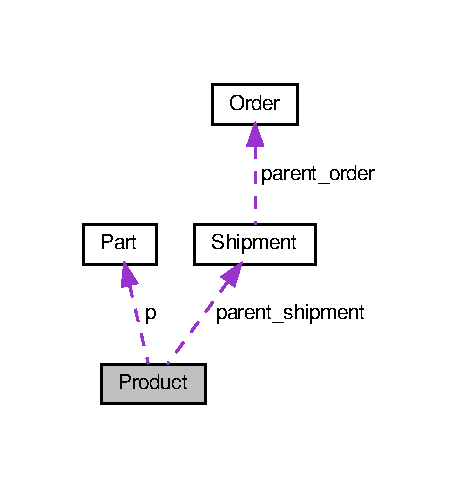
\includegraphics[width=221pt]{structProduct__coll__graph}
\end{center}
\end{figure}
\subsection*{Public Attributes}
\begin{DoxyCompactItemize}
\item 
\mbox{\Hypertarget{structProduct_a9794c822ffdfc304df2c70ba43af1916}\label{structProduct_a9794c822ffdfc304df2c70ba43af1916}} 
std\+::string {\bfseries type}
\item 
\mbox{\Hypertarget{structProduct_afdb4498246a795bdc91b8df0ba2f76b4}\label{structProduct_afdb4498246a795bdc91b8df0ba2f76b4}} 
geometry\+\_\+msgs\+::\+Pose {\bfseries pose}
\item 
\mbox{\Hypertarget{structProduct_a930e4b3e273598c534709f22cb1d4cac}\label{structProduct_a930e4b3e273598c534709f22cb1d4cac}} 
geometry\+\_\+msgs\+::\+Pose {\bfseries agv\+\_\+world\+\_\+pose}
\item 
\mbox{\Hypertarget{structProduct_a480966ce45a977dc57781b84e540292d}\label{structProduct_a480966ce45a977dc57781b84e540292d}} 
\hyperlink{utils_8h_a67ee3a5b9091664130eca8efc8b97ab9}{part} {\bfseries p}
\item 
\mbox{\Hypertarget{structProduct_a1a6ed448aeeed12f563d5ff05a26f936}\label{structProduct_a1a6ed448aeeed12f563d5ff05a26f936}} 
geometry\+\_\+msgs\+::\+Pose {\bfseries estimated\+\_\+conveyor\+\_\+pose}
\item 
\mbox{\Hypertarget{structProduct_a362e1bca7dacf78ca01aa09cba4bdbb1}\label{structProduct_a362e1bca7dacf78ca01aa09cba4bdbb1}} 
std\+::string {\bfseries agv\+\_\+id}
\item 
\mbox{\Hypertarget{structProduct_ab8ab1c46e9406bdb591c8b32c3d6bb5f}\label{structProduct_ab8ab1c46e9406bdb591c8b32c3d6bb5f}} 
std\+::string {\bfseries tray}
\item 
\mbox{\Hypertarget{structProduct_ab7b619e3758e153315fd6960d025a7ba}\label{structProduct_ab7b619e3758e153315fd6960d025a7ba}} 
std\+::string {\bfseries arm\+\_\+name}
\item 
\mbox{\Hypertarget{structProduct_aec6bebef64a095bd9ca08c3c1d107d2b}\label{structProduct_aec6bebef64a095bd9ca08c3c1d107d2b}} 
std\+::string {\bfseries cache\+\_\+id}
\item 
\mbox{\Hypertarget{structProduct_a6cdcd7f1ac8ef015c20baa1c93765885}\label{structProduct_a6cdcd7f1ac8ef015c20baa1c93765885}} 
\hyperlink{utils_8h_af15e89ebba88d2450b2866c705b15559}{shipment} $\ast$ {\bfseries parent\+\_\+shipment}
\item 
\mbox{\Hypertarget{structProduct_acf26204944fd9b2806361d166004ce26}\label{structProduct_acf26204944fd9b2806361d166004ce26}} 
bool {\bfseries high\+\_\+priority}
\item 
\mbox{\Hypertarget{structProduct_a81bc7bfb8798574d9b5f58dec68257e2}\label{structProduct_a81bc7bfb8798574d9b5f58dec68257e2}} 
int {\bfseries correction\+\_\+attempts}
\item 
\mbox{\Hypertarget{structProduct_abc4891099fad3ed0adc35ef02b5ef8be}\label{structProduct_abc4891099fad3ed0adc35ef02b5ef8be}} 
int {\bfseries service\+\_\+attempts}
\item 
\mbox{\Hypertarget{structProduct_a000b24f81adac8808f6bcbf02e68791f}\label{structProduct_a000b24f81adac8808f6bcbf02e68791f}} 
bool {\bfseries part\+\_\+placed} = false
\item 
\mbox{\Hypertarget{structProduct_a1a7bbf0dd07b412bce6eb12c3bb500ee}\label{structProduct_a1a7bbf0dd07b412bce6eb12c3bb500ee}} 
bool {\bfseries mv\+\_\+prod} = false
\item 
\mbox{\Hypertarget{structProduct_ae71dbd5781e7654476a95875105d6e58}\label{structProduct_ae71dbd5781e7654476a95875105d6e58}} 
int {\bfseries ship\+Id}
\item 
\mbox{\Hypertarget{structProduct_ade9eb069023303693749ca8dd75c83a5}\label{structProduct_ade9eb069023303693749ca8dd75c83a5}} 
std\+::vector$<$ double $>$ {\bfseries rpy\+\_\+final}
\item 
\mbox{\Hypertarget{structProduct_a2c245c65b7ee1dfbd23dcd3fcbe3e384}\label{structProduct_a2c245c65b7ee1dfbd23dcd3fcbe3e384}} 
float {\bfseries yaw\+\_\+correction} = 0
\end{DoxyCompactItemize}


\subsection{Detailed Description}
\hyperlink{structProduct}{Product} typedef. 

The documentation for this struct was generated from the following file\+:\begin{DoxyCompactItemize}
\item 
include/\hyperlink{utils_8h}{utils.\+h}\end{DoxyCompactItemize}

\hypertarget{structShipment}{}\section{Shipment Struct Reference}
\label{structShipment}\index{Shipment@{Shipment}}


\hyperlink{structShipment}{Shipment} typedef.  




{\ttfamily \#include $<$utils.\+h$>$}



Collaboration diagram for Shipment\+:\nopagebreak
\begin{figure}[H]
\begin{center}
\leavevmode
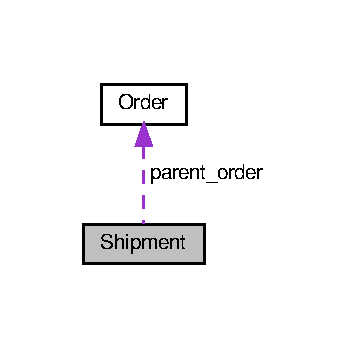
\includegraphics[width=167pt]{structShipment__coll__graph}
\end{center}
\end{figure}
\subsection*{Public Attributes}
\begin{DoxyCompactItemize}
\item 
\mbox{\Hypertarget{structShipment_afee83324bb0718df0bad07ddd6bfa698}\label{structShipment_afee83324bb0718df0bad07ddd6bfa698}} 
std\+::string {\bfseries shipment\+\_\+type}
\item 
\mbox{\Hypertarget{structShipment_a99c0e2efeb36ae051bebfee925076af1}\label{structShipment_a99c0e2efeb36ae051bebfee925076af1}} 
std\+::string {\bfseries agv\+\_\+id}
\item 
\mbox{\Hypertarget{structShipment_a549d2e4b2e90019d18e55110593e790f}\label{structShipment_a549d2e4b2e90019d18e55110593e790f}} 
std\+::vector$<$ \hyperlink{structProduct}{Product} $>$ {\bfseries products}
\item 
\mbox{\Hypertarget{structShipment_a3d5cdc2669ff03bb010989818e5e2369}\label{structShipment_a3d5cdc2669ff03bb010989818e5e2369}} 
int {\bfseries prod\+Complete} = 0
\item 
\mbox{\Hypertarget{structShipment_a1f5c06a24c0915d76b7bea80f3bd8d31}\label{structShipment_a1f5c06a24c0915d76b7bea80f3bd8d31}} 
\hyperlink{utils_8h_a88b083f4969e7c61a34a7231180f9e41}{order} $\ast$ {\bfseries parent\+\_\+order}
\item 
\mbox{\Hypertarget{structShipment_aac7fdf0f481c7ed76496a38f37d300ab}\label{structShipment_aac7fdf0f481c7ed76496a38f37d300ab}} 
int {\bfseries parent\+\_\+order\+\_\+idx}
\end{DoxyCompactItemize}


\subsection{Detailed Description}
\hyperlink{structShipment}{Shipment} typedef. 

The documentation for this struct was generated from the following file\+:\begin{DoxyCompactItemize}
\item 
include/\hyperlink{utils_8h}{utils.\+h}\end{DoxyCompactItemize}

\hypertarget{structsimilarParts}{}\section{similar\+Parts Struct Reference}
\label{structsimilarParts}\index{similar\+Parts@{similar\+Parts}}


Similar parts struct.  




{\ttfamily \#include $<$order\+Build.\+h$>$}



Collaboration diagram for similar\+Parts\+:
\nopagebreak
\begin{figure}[H]
\begin{center}
\leavevmode
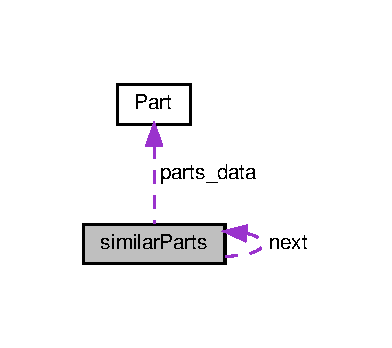
\includegraphics[width=188pt]{structsimilarParts__coll__graph}
\end{center}
\end{figure}
\subsection*{Public Attributes}
\begin{DoxyCompactItemize}
\item 
\mbox{\Hypertarget{structsimilarParts_a3f437349183287ca08b62bd3754c111c}\label{structsimilarParts_a3f437349183287ca08b62bd3754c111c}} 
\hyperlink{structPart}{Part} $\ast$ {\bfseries parts\+\_\+data}
\item 
\mbox{\Hypertarget{structsimilarParts_a715b323f6b367ed6b401279a9f68a090}\label{structsimilarParts_a715b323f6b367ed6b401279a9f68a090}} 
struct \hyperlink{structsimilarParts}{similar\+Parts} $\ast$ {\bfseries next}
\end{DoxyCompactItemize}


\subsection{Detailed Description}
Similar parts struct. 

The documentation for this struct was generated from the following file\+:\begin{DoxyCompactItemize}
\item 
include/\hyperlink{orderBuild_8h}{order\+Build.\+h}\end{DoxyCompactItemize}

\hypertarget{structStats}{}\section{Stats Struct Reference}
\label{structStats}\index{Stats@{Stats}}


\hyperlink{structStats}{Stats} typedef.  




{\ttfamily \#include $<$utils.\+h$>$}

\subsection*{Public Attributes}
\begin{DoxyCompactItemize}
\item 
\mbox{\Hypertarget{structStats_a70d36c1b69ef6756355c1203bc705c55}\label{structStats_a70d36c1b69ef6756355c1203bc705c55}} 
double {\bfseries total\+\_\+time} = 0.\+0
\item 
\mbox{\Hypertarget{structStats_aee859c4519969281cad6bf9ea94deb9a}\label{structStats_aee859c4519969281cad6bf9ea94deb9a}} 
double {\bfseries fail\+\_\+time} = 0.\+0
\item 
\mbox{\Hypertarget{structStats_a14faefc9acb2ce7d266c3673e37da7ee}\label{structStats_a14faefc9acb2ce7d266c3673e37da7ee}} 
int {\bfseries calls} = 0
\item 
\mbox{\Hypertarget{structStats_a24c80aca6cdab995eadceaec3a0a4803}\label{structStats_a24c80aca6cdab995eadceaec3a0a4803}} 
int {\bfseries fails} = 0
\end{DoxyCompactItemize}


\subsection{Detailed Description}
\hyperlink{structStats}{Stats} typedef. 

The documentation for this struct was generated from the following file\+:\begin{DoxyCompactItemize}
\item 
include/\hyperlink{utils_8h}{utils.\+h}\end{DoxyCompactItemize}

\chapter{File Documentation}
\hypertarget{competition_8h}{}\section{include/competition.h File Reference}
\label{competition_8h}\index{include/competition.\+h@{include/competition.\+h}}


Starts the A\+R\+I\+AC competition.  


{\ttfamily \#include $<$vector$>$}\newline
{\ttfamily \#include $<$ros/ros.\+h$>$}\newline
{\ttfamily \#include $<$stdio.\+h$>$}\newline
{\ttfamily \#include $<$std\+\_\+msgs/\+Float32.\+h$>$}\newline
{\ttfamily \#include $<$std\+\_\+msgs/\+String.\+h$>$}\newline
{\ttfamily \#include $<$rosgraph\+\_\+msgs/\+Clock.\+h$>$}\newline
{\ttfamily \#include $<$nist\+\_\+gear/\+Order.\+h$>$}\newline
{\ttfamily \#include \char`\"{}utils.\+h\char`\"{}}\newline
Include dependency graph for competition.\+h\+:\nopagebreak
\begin{figure}[H]
\begin{center}
\leavevmode
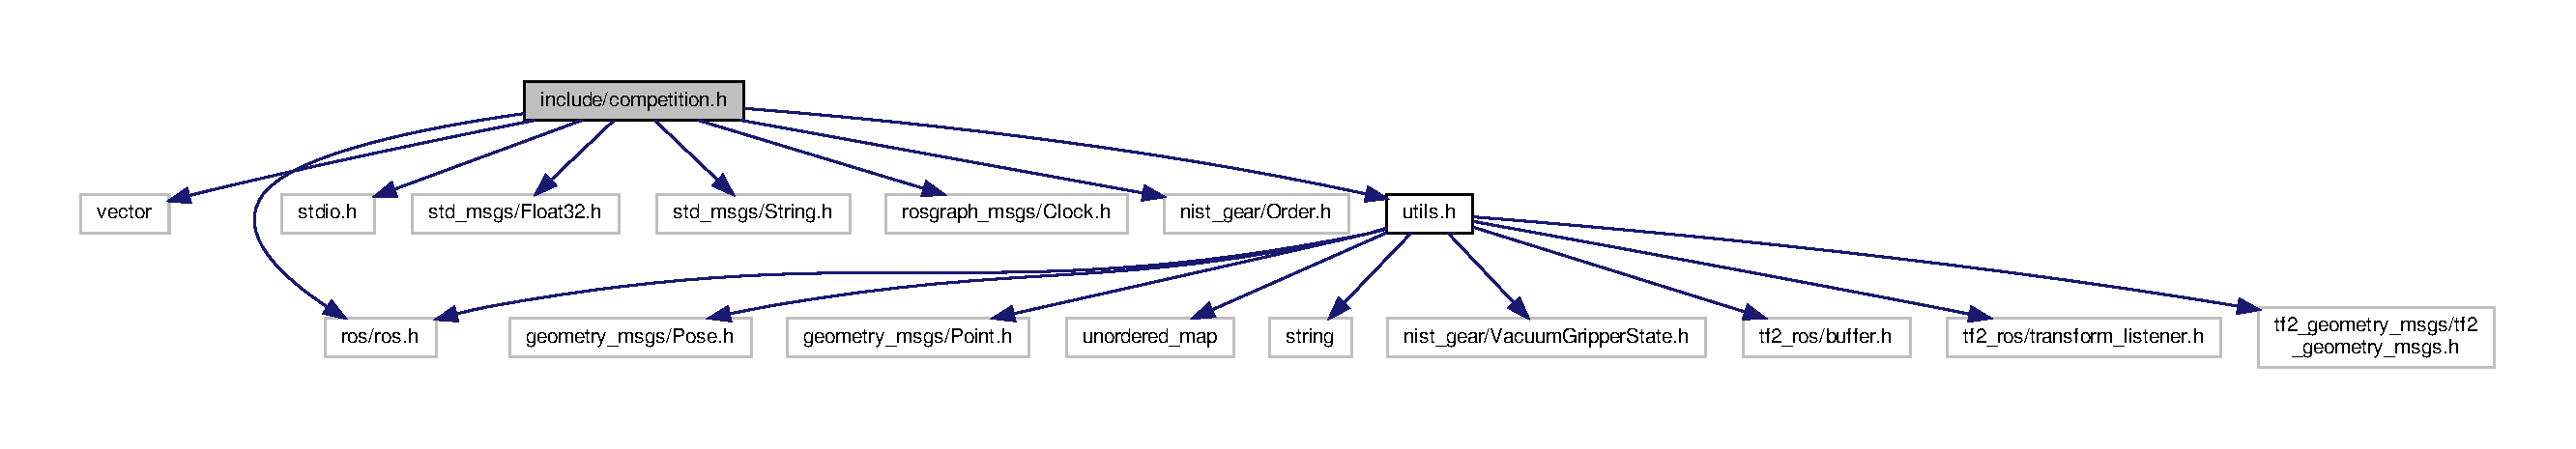
\includegraphics[width=350pt]{competition_8h__incl}
\end{center}
\end{figure}
This graph shows which files directly or indirectly include this file\+:\nopagebreak
\begin{figure}[H]
\begin{center}
\leavevmode
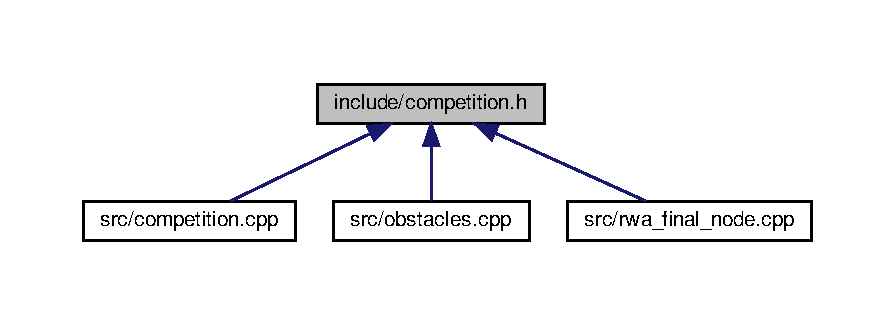
\includegraphics[width=350pt]{competition_8h__dep__incl}
\end{center}
\end{figure}
\subsection*{Classes}
\begin{DoxyCompactItemize}
\item 
class \hyperlink{classCompetition}{Competition}
\begin{DoxyCompactList}\small\item\em \hyperlink{classCompetition}{Competition} class. \end{DoxyCompactList}\end{DoxyCompactItemize}


\subsection{Detailed Description}
Starts the A\+R\+I\+AC competition. 

Copyright 2020 Nalin Das

\begin{DoxyAuthor}{Author}
Varun Asthana 

Saumil Shah 

Nalin Das 

Markose Jacob 

Aditya Goswami
\end{DoxyAuthor}
\begin{DoxyDate}{Date}
11/28/2020
\end{DoxyDate}
\hypertarget{utils_8cpp_DESCRIPTION}{}\subsection{D\+E\+S\+C\+R\+I\+P\+T\+I\+ON}\label{utils_8cpp_DESCRIPTION}
Header file containing A\+R\+I\+AC competition class 
\hypertarget{gantry__control_8h}{}\section{include/gantry\+\_\+control.h File Reference}
\label{gantry__control_8h}\index{include/gantry\+\_\+control.\+h@{include/gantry\+\_\+control.\+h}}


Gantry class.  


{\ttfamily \#include $<$ros/ros.\+h$>$}\newline
{\ttfamily \#include $<$std\+\_\+msgs/\+String.\+h$>$}\newline
{\ttfamily \#include $<$string$>$}\newline
{\ttfamily \#include $<$vector$>$}\newline
{\ttfamily \#include $<$ros/console.\+h$>$}\newline
{\ttfamily \#include $<$rosbag/bag.\+h$>$}\newline
{\ttfamily \#include $<$rosbag/view.\+h$>$}\newline
{\ttfamily \#include $<$array$>$}\newline
{\ttfamily \#include $<$moveit/move\+\_\+group\+\_\+interface/move\+\_\+group\+\_\+interface.\+h$>$}\newline
{\ttfamily \#include $<$moveit/planning\+\_\+scene\+\_\+interface/planning\+\_\+scene\+\_\+interface.\+h$>$}\newline
{\ttfamily \#include $<$moveit\+\_\+msgs/\+Display\+Robot\+State.\+h$>$}\newline
{\ttfamily \#include $<$moveit\+\_\+msgs/\+Display\+Trajectory.\+h$>$}\newline
{\ttfamily \#include $<$moveit\+\_\+msgs/\+Attached\+Collision\+Object.\+h$>$}\newline
{\ttfamily \#include $<$moveit\+\_\+msgs/\+Collision\+Object.\+h$>$}\newline
{\ttfamily \#include $<$moveit\+\_\+visual\+\_\+tools/moveit\+\_\+visual\+\_\+tools.\+h$>$}\newline
{\ttfamily \#include $<$boost/foreach.\+hpp$>$}\newline
{\ttfamily \#include $<$Eigen/\+Dense$>$}\newline
{\ttfamily \#include $<$tf2/\+Linear\+Math/\+Quaternion.\+h$>$}\newline
{\ttfamily \#include \char`\"{}geometric\+\_\+shapes/shapes.\+h\char`\"{}}\newline
{\ttfamily \#include \char`\"{}geometric\+\_\+shapes/mesh\+\_\+operations.\+h\char`\"{}}\newline
{\ttfamily \#include \char`\"{}geometric\+\_\+shapes/shape\+\_\+operations.\+h\char`\"{}}\newline
{\ttfamily \#include $<$nist\+\_\+gear/\+Vacuum\+Gripper\+State.\+h$>$}\newline
{\ttfamily \#include $<$nist\+\_\+gear/\+Vacuum\+Gripper\+Control.\+h$>$}\newline
{\ttfamily \#include $<$sensor\+\_\+msgs/\+Joint\+State.\+h$>$}\newline
{\ttfamily \#include $<$control\+\_\+msgs/\+Joint\+Trajectory\+Controller\+State.\+h$>$}\newline
{\ttfamily \#include $<$trajectory\+\_\+msgs/\+Joint\+Trajectory.\+h$>$}\newline
{\ttfamily \#include \char`\"{}utils.\+h\char`\"{}}\newline
{\ttfamily \#include \char`\"{}order\+Build.\+h\char`\"{}}\newline
{\ttfamily \#include \char`\"{}conveyer.\+h\char`\"{}}\newline
{\ttfamily \#include \char`\"{}obstacles.\+h\char`\"{}}\newline
{\ttfamily \#include $<$nist\+\_\+gear/\+Logical\+Camera\+Image.\+h$>$}\newline
Include dependency graph for gantry\+\_\+control.\+h\+:\nopagebreak
\begin{figure}[H]
\begin{center}
\leavevmode
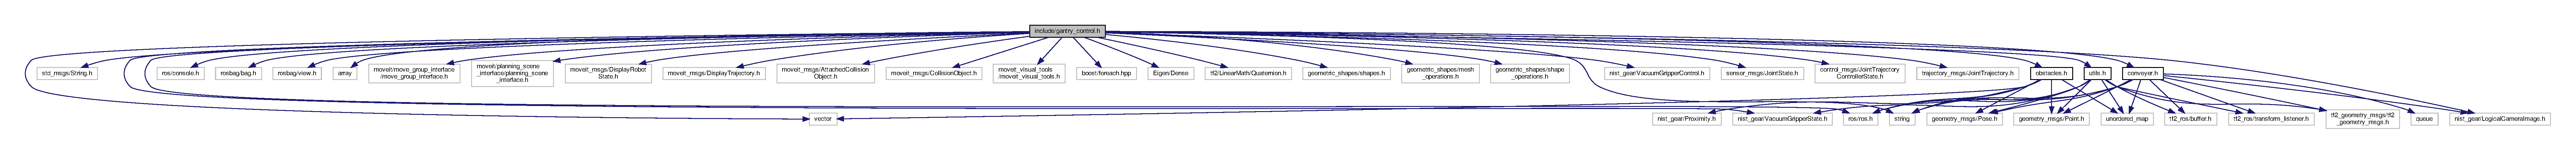
\includegraphics[width=350pt]{gantry__control_8h__incl}
\end{center}
\end{figure}
This graph shows which files directly or indirectly include this file\+:\nopagebreak
\begin{figure}[H]
\begin{center}
\leavevmode
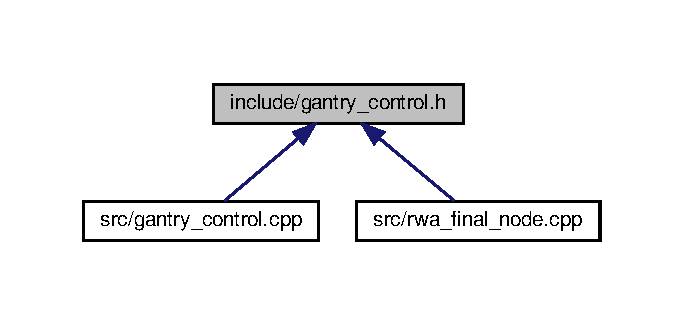
\includegraphics[width=328pt]{gantry__control_8h__dep__incl}
\end{center}
\end{figure}
\subsection*{Classes}
\begin{DoxyCompactItemize}
\item 
class \hyperlink{classGantryControl}{Gantry\+Control}
\begin{DoxyCompactList}\small\item\em Gantry Control class. \end{DoxyCompactList}\end{DoxyCompactItemize}
\subsection*{Macros}
\begin{DoxyCompactItemize}
\item 
\mbox{\Hypertarget{gantry__control_8h_a85d9ac269eba33293361f4ed7c2a697b}\label{gantry__control_8h_a85d9ac269eba33293361f4ed7c2a697b}} 
\#define {\bfseries foreach}~B\+O\+O\+S\+T\+\_\+\+F\+O\+R\+E\+A\+CH
\end{DoxyCompactItemize}


\subsection{Detailed Description}
Gantry class. 

Copyright 2020 Nalin Das

\begin{DoxyAuthor}{Author}
Varun Asthana 

Saumil Shah 

Nalin Das 

Markose Jacob 

Aditya Goswami
\end{DoxyAuthor}
\begin{DoxyDate}{Date}
11/28/2020
\end{DoxyDate}
\hypertarget{utils_8cpp_DESCRIPTION}{}\subsection{D\+E\+S\+C\+R\+I\+P\+T\+I\+ON}\label{utils_8cpp_DESCRIPTION}
Header file for the Gantry Control class 
\hypertarget{obstacles_8h}{}\section{include/obstacles.h File Reference}
\label{obstacles_8h}\index{include/obstacles.\+h@{include/obstacles.\+h}}


\hyperlink{classObstaclesInAisle}{Obstacles\+In\+Aisle} class.  


{\ttfamily \#include $<$geometry\+\_\+msgs/\+Pose.\+h$>$}\newline
{\ttfamily \#include $<$geometry\+\_\+msgs/\+Point.\+h$>$}\newline
{\ttfamily \#include $<$string$>$}\newline
{\ttfamily \#include $<$vector$>$}\newline
{\ttfamily \#include $<$ros/ros.\+h$>$}\newline
{\ttfamily \#include $<$nist\+\_\+gear/\+Proximity.\+h$>$}\newline
{\ttfamily \#include $<$unordered\+\_\+map$>$}\newline
Include dependency graph for obstacles.\+h\+:
\nopagebreak
\begin{figure}[H]
\begin{center}
\leavevmode
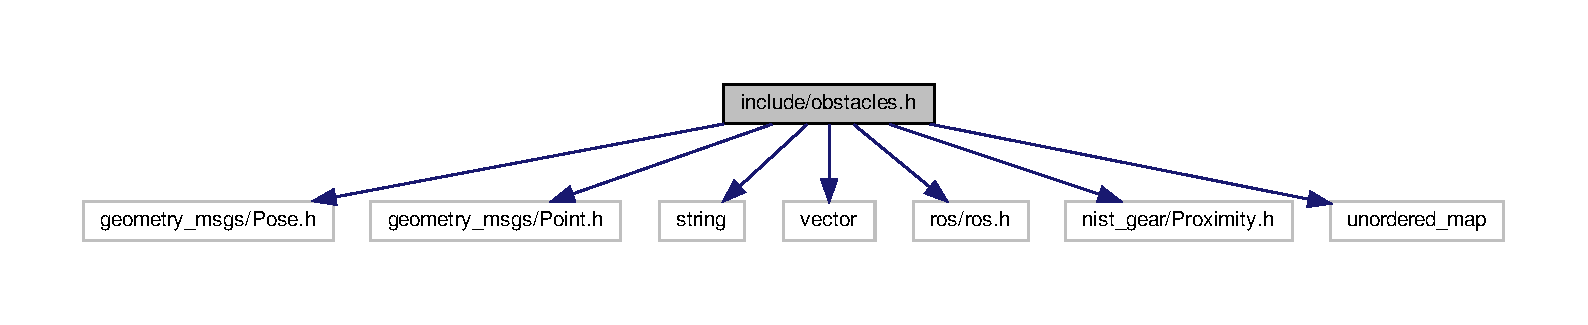
\includegraphics[width=350pt]{obstacles_8h__incl}
\end{center}
\end{figure}
This graph shows which files directly or indirectly include this file\+:
\nopagebreak
\begin{figure}[H]
\begin{center}
\leavevmode
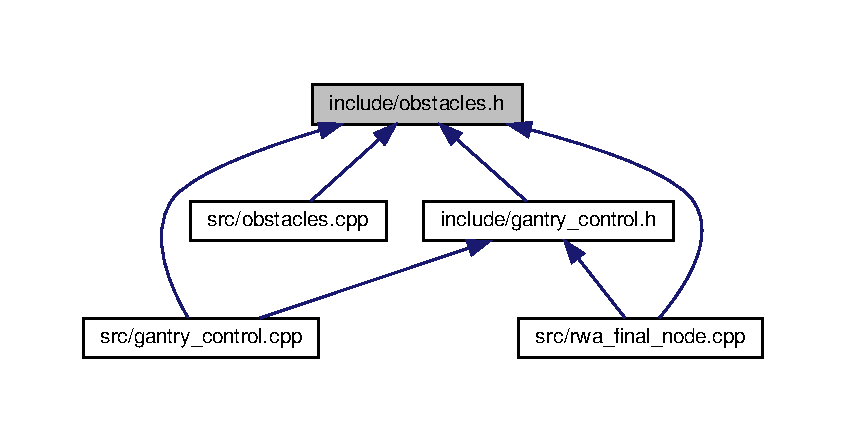
\includegraphics[width=350pt]{obstacles_8h__dep__incl}
\end{center}
\end{figure}
\subsection*{Classes}
\begin{DoxyCompactItemize}
\item 
class \hyperlink{classObstaclesInAisle}{Obstacles\+In\+Aisle}
\begin{DoxyCompactList}\small\item\em \hyperlink{classObstaclesInAisle}{Obstacles\+In\+Aisle} class. \end{DoxyCompactList}\end{DoxyCompactItemize}


\subsection{Detailed Description}
\hyperlink{classObstaclesInAisle}{Obstacles\+In\+Aisle} class. 

Copyright 2020 Varun Asthana, Saumil Shah, Nalin Das, Markose Jacob, Aditya Goswami

\begin{DoxyAuthor}{Author}
Varun Asthana 

Saumil Shah 

Nalin Das 

Markose Jacob 

Aditya Goswami
\end{DoxyAuthor}
\begin{DoxyDate}{Date}
11/29/2020
\end{DoxyDate}
\hypertarget{utils_8cpp_DESCRIPTION}{}\subsection{D\+E\+S\+C\+R\+I\+P\+T\+I\+ON}\label{utils_8cpp_DESCRIPTION}
Header file for the \hyperlink{classObstaclesInAisle}{Obstacles\+In\+Aisle} class 
\hypertarget{orderBuild_8h}{}\section{include/order\+Build.h File Reference}
\label{orderBuild_8h}\index{include/order\+Build.\+h@{include/order\+Build.\+h}}


\hyperlink{classBuildClass}{Build\+Class} and \hyperlink{classallStaticParts}{all\+Static\+Parts} class.  


{\ttfamily \#include $<$ros/ros.\+h$>$}\newline
{\ttfamily \#include $<$nist\+\_\+gear/\+Logical\+Camera\+Image.\+h$>$}\newline
{\ttfamily \#include $<$nist\+\_\+gear/\+Order.\+h$>$}\newline
{\ttfamily \#include \char`\"{}utils.\+h\char`\"{}}\newline
{\ttfamily \#include \char`\"{}conveyer.\+h\char`\"{}}\newline
{\ttfamily \#include $<$utility$>$}\newline
Include dependency graph for order\+Build.\+h\+:
\nopagebreak
\begin{figure}[H]
\begin{center}
\leavevmode
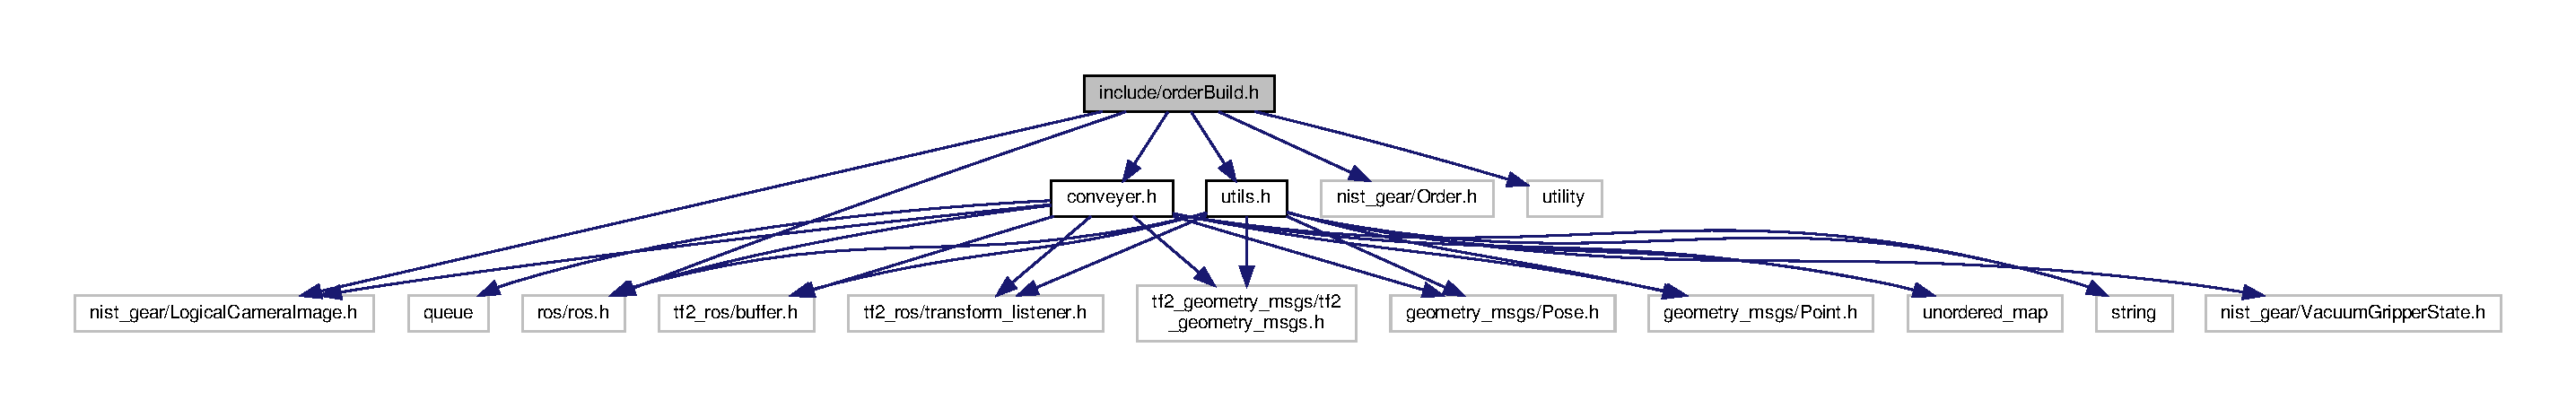
\includegraphics[width=350pt]{orderBuild_8h__incl}
\end{center}
\end{figure}
This graph shows which files directly or indirectly include this file\+:
\nopagebreak
\begin{figure}[H]
\begin{center}
\leavevmode
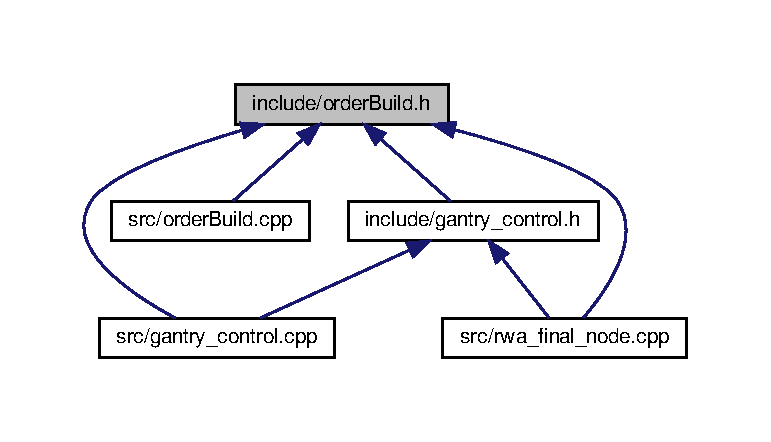
\includegraphics[width=350pt]{orderBuild_8h__dep__incl}
\end{center}
\end{figure}
\subsection*{Classes}
\begin{DoxyCompactItemize}
\item 
struct \hyperlink{structsimilarParts}{similar\+Parts}
\begin{DoxyCompactList}\small\item\em Similar parts struct. \end{DoxyCompactList}\item 
class \hyperlink{classallStaticParts}{all\+Static\+Parts}
\begin{DoxyCompactList}\small\item\em \hyperlink{classallStaticParts}{all\+Static\+Parts} Class \end{DoxyCompactList}\item 
class \hyperlink{classBuildClass}{Build\+Class}
\begin{DoxyCompactList}\small\item\em Build class. \end{DoxyCompactList}\end{DoxyCompactItemize}


\subsection{Detailed Description}
\hyperlink{classBuildClass}{Build\+Class} and \hyperlink{classallStaticParts}{all\+Static\+Parts} class. 

Copyright 2020 Varun Asthana, Saumil Shah, Nalin Das, Markose Jacob, Aditya Goswami

\begin{DoxyAuthor}{Author}
Varun Asthana 

Saumil Shah 

Nalin Das 

Markose Jacob 

Aditya Goswami
\end{DoxyAuthor}
\begin{DoxyDate}{Date}
11/29/2020
\end{DoxyDate}
\hypertarget{utils_8cpp_DESCRIPTION}{}\subsection{D\+E\+S\+C\+R\+I\+P\+T\+I\+ON}\label{utils_8cpp_DESCRIPTION}
Header file for the \hyperlink{classBuildClass}{Build\+Class} and \hyperlink{classallStaticParts}{all\+Static\+Parts} class 
\hypertarget{utils_8h}{}\section{include/utils.h File Reference}
\label{utils_8h}\index{include/utils.\+h@{include/utils.\+h}}


Contains general utility typedefs.  


{\ttfamily \#include $<$geometry\+\_\+msgs/\+Pose.\+h$>$}\newline
{\ttfamily \#include $<$geometry\+\_\+msgs/\+Point.\+h$>$}\newline
{\ttfamily \#include $<$unordered\+\_\+map$>$}\newline
{\ttfamily \#include $<$string$>$}\newline
{\ttfamily \#include $<$ros/ros.\+h$>$}\newline
{\ttfamily \#include $<$nist\+\_\+gear/\+Vacuum\+Gripper\+State.\+h$>$}\newline
{\ttfamily \#include $<$tf2\+\_\+ros/buffer.\+h$>$}\newline
{\ttfamily \#include $<$tf2\+\_\+ros/transform\+\_\+listener.\+h$>$}\newline
{\ttfamily \#include $<$tf2\+\_\+geometry\+\_\+msgs/tf2\+\_\+geometry\+\_\+msgs.\+h$>$}\newline
Include dependency graph for utils.\+h\+:
\nopagebreak
\begin{figure}[H]
\begin{center}
\leavevmode
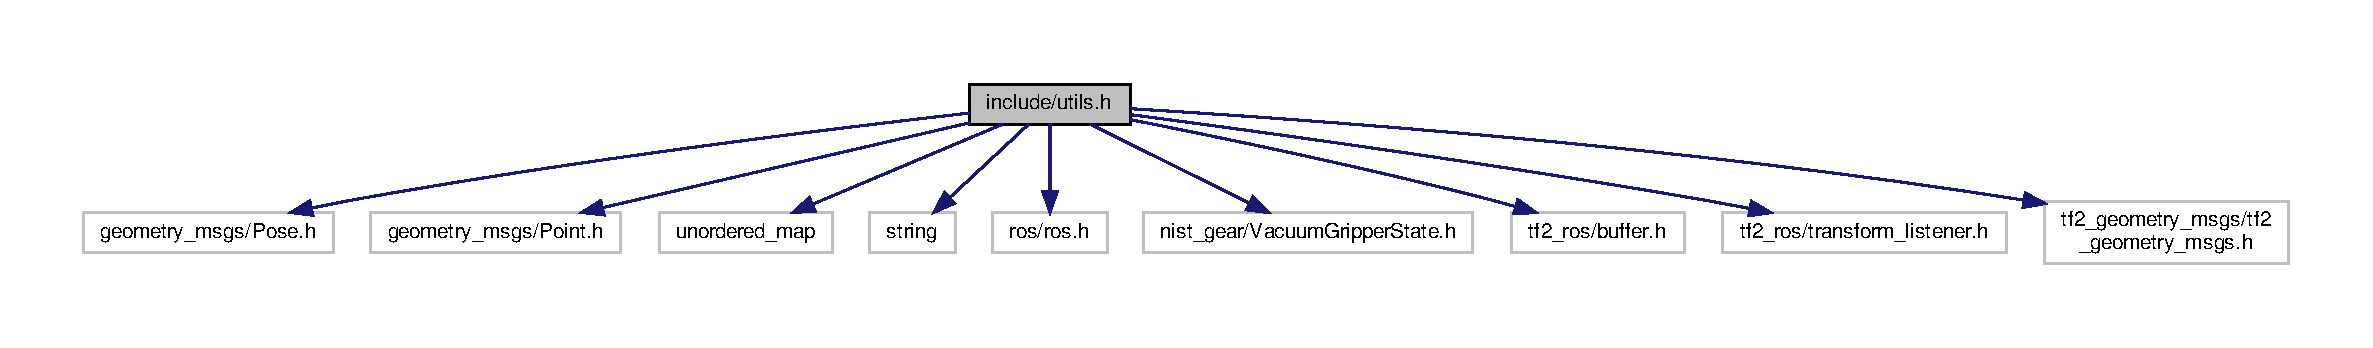
\includegraphics[width=350pt]{utils_8h__incl}
\end{center}
\end{figure}
This graph shows which files directly or indirectly include this file\+:
\nopagebreak
\begin{figure}[H]
\begin{center}
\leavevmode
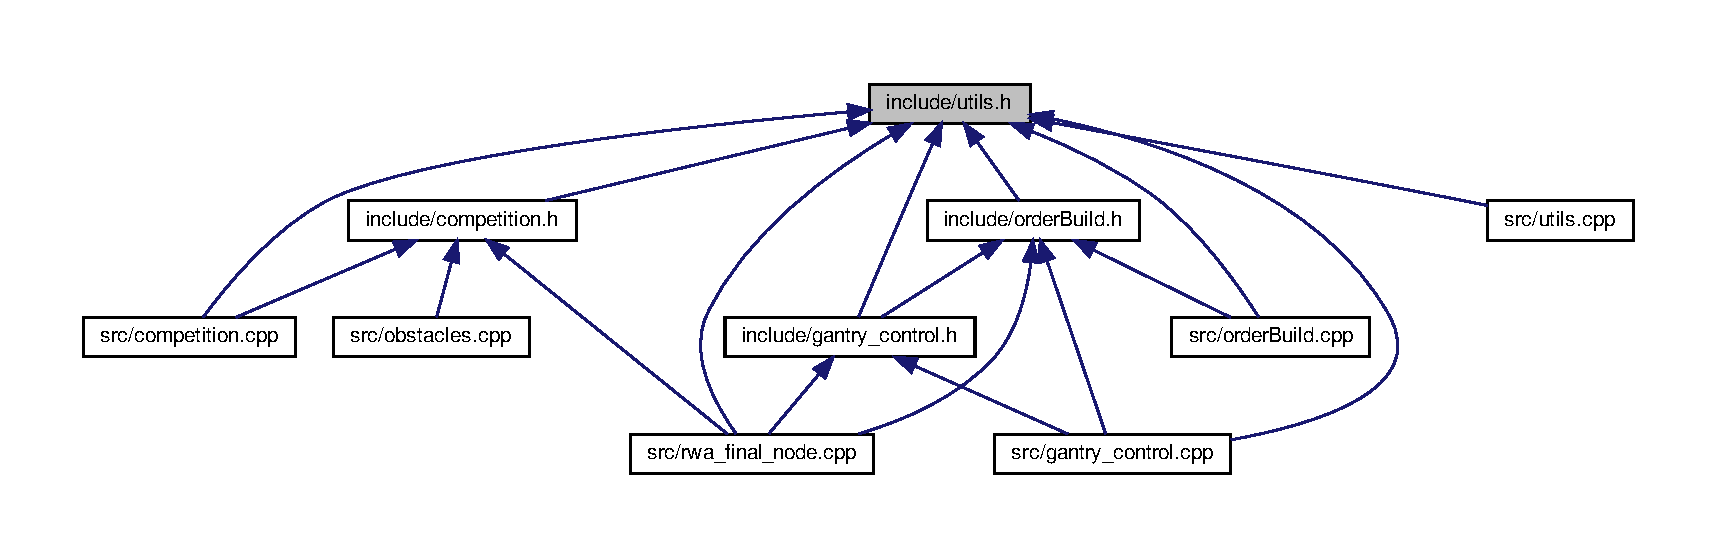
\includegraphics[width=350pt]{utils_8h__dep__incl}
\end{center}
\end{figure}
\subsection*{Classes}
\begin{DoxyCompactItemize}
\item 
struct \hyperlink{structPresetLocation}{Preset\+Location}
\begin{DoxyCompactList}\small\item\em Preset Location typedef. \end{DoxyCompactList}\item 
struct \hyperlink{structPart}{Part}
\begin{DoxyCompactList}\small\item\em \hyperlink{structPart}{Part} typedef. \end{DoxyCompactList}\item 
struct \hyperlink{structPosition}{Position}
\begin{DoxyCompactList}\small\item\em \hyperlink{structPosition}{Position} typedef. \end{DoxyCompactList}\item 
struct \hyperlink{structShipment}{Shipment}
\begin{DoxyCompactList}\small\item\em \hyperlink{structShipment}{Shipment} typedef. \end{DoxyCompactList}\item 
struct \hyperlink{structProduct}{Product}
\begin{DoxyCompactList}\small\item\em \hyperlink{structProduct}{Product} typedef. \end{DoxyCompactList}\item 
struct \hyperlink{structOrder}{Order}
\begin{DoxyCompactList}\small\item\em \hyperlink{structOrder}{Order} typedef. \end{DoxyCompactList}\item 
struct \hyperlink{structStats}{Stats}
\begin{DoxyCompactList}\small\item\em \hyperlink{structStats}{Stats} typedef. \end{DoxyCompactList}\item 
struct \hyperlink{structall__Order}{all\+\_\+\+Order}
\begin{DoxyCompactList}\small\item\em All orders struct. \end{DoxyCompactList}\item 
struct \hyperlink{structagvInfo}{agv\+Info}
\begin{DoxyCompactList}\small\item\em A\+GV Information struct. \end{DoxyCompactList}\end{DoxyCompactItemize}
\subsection*{Typedefs}
\begin{DoxyCompactItemize}
\item 
typedef struct \hyperlink{structShipment}{Shipment} \hyperlink{utils_8h_af15e89ebba88d2450b2866c705b15559}{shipment}
\begin{DoxyCompactList}\small\item\em \hyperlink{structShipment}{Shipment} struct object. \end{DoxyCompactList}\item 
typedef struct \hyperlink{structOrder}{Order} \hyperlink{utils_8h_a88b083f4969e7c61a34a7231180f9e41}{order}
\begin{DoxyCompactList}\small\item\em Object struct object. \end{DoxyCompactList}\item 
typedef struct \hyperlink{structProduct}{Product} \hyperlink{utils_8h_a48a7207852c0455cce7e65703b12ec7e}{product}
\begin{DoxyCompactList}\small\item\em \hyperlink{structProduct}{Product} struct object. \end{DoxyCompactList}\item 
\mbox{\Hypertarget{utils_8h_a36494ad089a17d7ae00c4cc799ed0970}\label{utils_8h_a36494ad089a17d7ae00c4cc799ed0970}} 
typedef struct \hyperlink{structPresetLocation}{Preset\+Location} \hyperlink{utils_8h_a36494ad089a17d7ae00c4cc799ed0970}{start}
\begin{DoxyCompactList}\small\item\em Preset Location typedef. \end{DoxyCompactList}\item 
\mbox{\Hypertarget{utils_8h_a44799e750ff70c96e6da44b750d28504}\label{utils_8h_a44799e750ff70c96e6da44b750d28504}} 
typedef struct \hyperlink{structPresetLocation}{Preset\+Location} {\bfseries bin3}
\item 
\mbox{\Hypertarget{utils_8h_a07d4041d68ff8967b0030f72d7f6671a}\label{utils_8h_a07d4041d68ff8967b0030f72d7f6671a}} 
typedef struct \hyperlink{structPresetLocation}{Preset\+Location} {\bfseries agv1}
\item 
\mbox{\Hypertarget{utils_8h_a20c31ccc433318f0c29e1f143206cca7}\label{utils_8h_a20c31ccc433318f0c29e1f143206cca7}} 
typedef struct \hyperlink{structPresetLocation}{Preset\+Location} {\bfseries agv2}
\item 
\mbox{\Hypertarget{utils_8h_ac68ff98e1a4c6dc8c303bef9e7434681}\label{utils_8h_ac68ff98e1a4c6dc8c303bef9e7434681}} 
typedef struct \hyperlink{structPresetLocation}{Preset\+Location} {\bfseries flipped\+\_\+pulley}
\item 
\mbox{\Hypertarget{utils_8h_a116eaae25b61b26d0f6d86ea7b1868e9}\label{utils_8h_a116eaae25b61b26d0f6d86ea7b1868e9}} 
typedef struct \hyperlink{structPresetLocation}{Preset\+Location} {\bfseries conveyor\+\_\+up}
\item 
\mbox{\Hypertarget{utils_8h_a67ee3a5b9091664130eca8efc8b97ab9}\label{utils_8h_a67ee3a5b9091664130eca8efc8b97ab9}} 
typedef struct \hyperlink{structPart}{Part} \hyperlink{utils_8h_a67ee3a5b9091664130eca8efc8b97ab9}{part}
\begin{DoxyCompactList}\small\item\em \hyperlink{structPart}{Part} typedef. \end{DoxyCompactList}\item 
\mbox{\Hypertarget{utils_8h_ac33d19e14b97838596178faf9194d5e2}\label{utils_8h_ac33d19e14b97838596178faf9194d5e2}} 
typedef struct \hyperlink{structPosition}{Position} \hyperlink{utils_8h_ac33d19e14b97838596178faf9194d5e2}{position}
\begin{DoxyCompactList}\small\item\em \hyperlink{structPosition}{Position} typedef. \end{DoxyCompactList}\item 
\mbox{\Hypertarget{utils_8h_abd807f196b951c0cdd24d50164d54763}\label{utils_8h_abd807f196b951c0cdd24d50164d54763}} 
typedef struct \hyperlink{structStats}{Stats} \hyperlink{utils_8h_abd807f196b951c0cdd24d50164d54763}{stats}
\begin{DoxyCompactList}\small\item\em \hyperlink{structStats}{Stats} typedef. \end{DoxyCompactList}\end{DoxyCompactItemize}
\subsection*{Enumerations}
\begin{DoxyCompactItemize}
\item 
\mbox{\Hypertarget{utils_8h_aaf7e202ccc2e0bac6d05d124e49b11d3}\label{utils_8h_aaf7e202ccc2e0bac6d05d124e49b11d3}} 
enum \hyperlink{utils_8h_aaf7e202ccc2e0bac6d05d124e49b11d3}{Part\+States} \{ \newline
{\bfseries F\+R\+EE}, 
{\bfseries B\+O\+O\+K\+ED}, 
{\bfseries U\+N\+R\+E\+A\+C\+H\+A\+B\+LE}, 
{\bfseries O\+N\+\_\+\+T\+R\+AY}, 
\newline
{\bfseries G\+R\+I\+P\+P\+ED}, 
{\bfseries G\+O\+I\+N\+G\+\_\+\+H\+O\+ME}, 
{\bfseries R\+E\+M\+O\+V\+E\+\_\+\+F\+R\+O\+M\+\_\+\+T\+R\+AY}, 
{\bfseries L\+O\+ST}
 \}\begin{DoxyCompactList}\small\item\em \hyperlink{structPart}{Part} states. \end{DoxyCompactList}
\end{DoxyCompactItemize}
\subsection*{Functions}
\begin{DoxyCompactItemize}
\item 
std\+::vector$<$ double $>$ \hyperlink{utils_8h_a6296f07aa6ba20f987431f971ffd77b9}{quaternion\+To\+Euler} (geometry\+\_\+msgs\+::\+Pose pose)
\begin{DoxyCompactList}\small\item\em Quaternion To Euler function. \end{DoxyCompactList}\item 
bool \hyperlink{utils_8h_a395ab737d890071e60aa28796372be0f}{is\+Aisle\+Clear} (int aisle\+\_\+num)
\begin{DoxyCompactList}\small\item\em Checks if aisle is clear. \end{DoxyCompactList}\end{DoxyCompactItemize}
\subsection*{Variables}
\begin{DoxyCompactItemize}
\item 
\mbox{\Hypertarget{utils_8h_a952eac791b596a61bba0a133a3bb439f}\label{utils_8h_a952eac791b596a61bba0a133a3bb439f}} 
const double {\bfseries PI} = 3.\+141592
\item 
\mbox{\Hypertarget{utils_8h_a5db325f306a804d4fee12e3ad0d39d96}\label{utils_8h_a5db325f306a804d4fee12e3ad0d39d96}} 
const int \hyperlink{utils_8h_a5db325f306a804d4fee12e3ad0d39d96}{M\+A\+X\+\_\+\+N\+U\+M\+B\+E\+R\+\_\+\+O\+F\+\_\+\+C\+A\+M\+E\+R\+AS} = 17
\begin{DoxyCompactList}\small\item\em Max Number of logical cameras. \end{DoxyCompactList}\item 
\mbox{\Hypertarget{utils_8h_a90cee088fb10cf6717fec7eb20aee725}\label{utils_8h_a90cee088fb10cf6717fec7eb20aee725}} 
const int \hyperlink{utils_8h_a90cee088fb10cf6717fec7eb20aee725}{M\+A\+X\+\_\+\+P\+I\+C\+K\+I\+N\+G\+\_\+\+A\+T\+T\+E\+M\+P\+TS} = 3
\begin{DoxyCompactList}\small\item\em Maximum picking attempts. \end{DoxyCompactList}\item 
\mbox{\Hypertarget{utils_8h_af49bd256f294b2ef350ec879bcce88f1}\label{utils_8h_af49bd256f294b2ef350ec879bcce88f1}} 
const double \hyperlink{utils_8h_af49bd256f294b2ef350ec879bcce88f1}{A\+B\+O\+V\+E\+\_\+\+T\+A\+R\+G\+ET} = 0.\+1
\begin{DoxyCompactList}\small\item\em Above target z pos when picking/placing part. \end{DoxyCompactList}\item 
\mbox{\Hypertarget{utils_8h_a903b8785bcd1d36cef1a0fdc52cd43b3}\label{utils_8h_a903b8785bcd1d36cef1a0fdc52cd43b3}} 
const double \hyperlink{utils_8h_a903b8785bcd1d36cef1a0fdc52cd43b3}{P\+I\+C\+K\+\_\+\+T\+I\+M\+E\+O\+UT} = 4.\+0
\begin{DoxyCompactList}\small\item\em Pickup Timeout. \end{DoxyCompactList}\item 
\mbox{\Hypertarget{utils_8h_a810037d8e3661f8fba6182e550fada34}\label{utils_8h_a810037d8e3661f8fba6182e550fada34}} 
const double \hyperlink{utils_8h_a810037d8e3661f8fba6182e550fada34}{R\+E\+T\+R\+I\+E\+V\+E\+\_\+\+T\+I\+M\+E\+O\+UT} = 2.\+0
\begin{DoxyCompactList}\small\item\em Retrieve Timeout. \end{DoxyCompactList}\item 
\mbox{\Hypertarget{utils_8h_ad0c4f19278f08a8e1859b67e7c29a481}\label{utils_8h_ad0c4f19278f08a8e1859b67e7c29a481}} 
const double \hyperlink{utils_8h_ad0c4f19278f08a8e1859b67e7c29a481}{B\+E\+L\+T\+\_\+\+S\+P\+E\+ED} = 0.\+2
\begin{DoxyCompactList}\small\item\em Belt Speed in m/s. \end{DoxyCompactList}\item 
\mbox{\Hypertarget{utils_8h_aa4641c377cd847a8e8625e8419265dd1}\label{utils_8h_aa4641c377cd847a8e8625e8419265dd1}} 
const double \hyperlink{utils_8h_aa4641c377cd847a8e8625e8419265dd1}{G\+R\+I\+P\+P\+E\+R\+\_\+\+H\+E\+I\+G\+HT} = 0.\+01
\begin{DoxyCompactList}\small\item\em Gripper Height. \end{DoxyCompactList}\item 
\mbox{\Hypertarget{utils_8h_a596344e5a2992d2beec43b76a6294de0}\label{utils_8h_a596344e5a2992d2beec43b76a6294de0}} 
const double \hyperlink{utils_8h_a596344e5a2992d2beec43b76a6294de0}{E\+P\+S\+I\+L\+ON} = 0.\+01
\begin{DoxyCompactList}\small\item\em Epsilon for the gripper to firmly touch. \end{DoxyCompactList}\item 
\mbox{\Hypertarget{utils_8h_a77876460e2cb342aa6783c5fda04ef5c}\label{utils_8h_a77876460e2cb342aa6783c5fda04ef5c}} 
const double \hyperlink{utils_8h_a77876460e2cb342aa6783c5fda04ef5c}{B\+I\+N\+\_\+\+H\+E\+I\+G\+HT} = 0.\+724
\begin{DoxyCompactList}\small\item\em Bin Height. \end{DoxyCompactList}\item 
\mbox{\Hypertarget{utils_8h_a094f5efa5987e6e53c7ecbe2a8bdf7cc}\label{utils_8h_a094f5efa5987e6e53c7ecbe2a8bdf7cc}} 
const double \hyperlink{utils_8h_a094f5efa5987e6e53c7ecbe2a8bdf7cc}{T\+R\+A\+Y\+\_\+\+H\+E\+I\+G\+HT} = 0.\+755
\begin{DoxyCompactList}\small\item\em Tray Height. \end{DoxyCompactList}\item 
\mbox{\Hypertarget{utils_8h_a39c6028d8032823b175d86b2053ee13c}\label{utils_8h_a39c6028d8032823b175d86b2053ee13c}} 
const double \hyperlink{utils_8h_a39c6028d8032823b175d86b2053ee13c}{R\+A\+I\+L\+\_\+\+H\+E\+I\+G\+HT} = 0.\+95
\begin{DoxyCompactList}\small\item\em Rail Height. \end{DoxyCompactList}\item 
\mbox{\Hypertarget{utils_8h_a9d3410770ee083c74e767d72261a798f}\label{utils_8h_a9d3410770ee083c74e767d72261a798f}} 
const double \hyperlink{utils_8h_a9d3410770ee083c74e767d72261a798f}{P\+L\+A\+N\+N\+I\+N\+G\+\_\+\+T\+I\+ME} = 20
\begin{DoxyCompactList}\small\item\em Planning\+\_\+\+Time for move\+\_\+group. \end{DoxyCompactList}\item 
\mbox{\Hypertarget{utils_8h_a429e859a3b7d55b6dcfdf308af80f473}\label{utils_8h_a429e859a3b7d55b6dcfdf308af80f473}} 
const int \hyperlink{utils_8h_a429e859a3b7d55b6dcfdf308af80f473}{M\+A\+X\+\_\+\+E\+X\+C\+H\+A\+N\+G\+E\+\_\+\+A\+T\+T\+E\+M\+P\+TS} = 6
\begin{DoxyCompactList}\small\item\em Max Exchange Attempts. \end{DoxyCompactList}\item 
\mbox{\Hypertarget{utils_8h_a1fe773a5a64450e78e8e4ab7adbf4ecb}\label{utils_8h_a1fe773a5a64450e78e8e4ab7adbf4ecb}} 
std\+::string \hyperlink{utils_8h_a1fe773a5a64450e78e8e4ab7adbf4ecb}{action\+\_\+state\+\_\+name} \mbox{[}$\,$\mbox{]}
\begin{DoxyCompactList}\small\item\em Action state name. \end{DoxyCompactList}\item 
\mbox{\Hypertarget{utils_8h_a4443f04d04826b4cb4d695dadc9a3a03}\label{utils_8h_a4443f04d04826b4cb4d695dadc9a3a03}} 
std\+::unordered\+\_\+map$<$ std\+::string, double $>$ \hyperlink{utils_8h_a4443f04d04826b4cb4d695dadc9a3a03}{model\+\_\+height}
\begin{DoxyCompactList}\small\item\em Model height hashmap. \end{DoxyCompactList}\end{DoxyCompactItemize}


\subsection{Detailed Description}
Contains general utility typedefs. 

Copyright 2020 Varun Asthana, Saumil Shah, Nalin Das, Markose Jacob, Aditya Goswami

\begin{DoxyAuthor}{Author}
Varun Asthana 

Saumil Shah 

Nalin Das 

Markose Jacob 

Aditya Goswami
\end{DoxyAuthor}
\begin{DoxyDate}{Date}
11/29/2020
\end{DoxyDate}
\hypertarget{utils_8cpp_DESCRIPTION}{}\subsection{D\+E\+S\+C\+R\+I\+P\+T\+I\+ON}\label{utils_8cpp_DESCRIPTION}
Header file for utility typedefs 

\subsection{Typedef Documentation}
\mbox{\Hypertarget{utils_8h_a88b083f4969e7c61a34a7231180f9e41}\label{utils_8h_a88b083f4969e7c61a34a7231180f9e41}} 
\index{utils.\+h@{utils.\+h}!order@{order}}
\index{order@{order}!utils.\+h@{utils.\+h}}
\subsubsection{\texorpdfstring{order}{order}}
{\footnotesize\ttfamily typedef struct \hyperlink{structOrder}{Order} \hyperlink{utils_8h_a88b083f4969e7c61a34a7231180f9e41}{order}}



Object struct object. 

\hyperlink{structOrder}{Order} typedef. \mbox{\Hypertarget{utils_8h_a48a7207852c0455cce7e65703b12ec7e}\label{utils_8h_a48a7207852c0455cce7e65703b12ec7e}} 
\index{utils.\+h@{utils.\+h}!product@{product}}
\index{product@{product}!utils.\+h@{utils.\+h}}
\subsubsection{\texorpdfstring{product}{product}}
{\footnotesize\ttfamily typedef struct \hyperlink{structProduct}{Product} \hyperlink{utils_8h_a48a7207852c0455cce7e65703b12ec7e}{product}}



\hyperlink{structProduct}{Product} struct object. 

\hyperlink{structProduct}{Product} typedef. \mbox{\Hypertarget{utils_8h_af15e89ebba88d2450b2866c705b15559}\label{utils_8h_af15e89ebba88d2450b2866c705b15559}} 
\index{utils.\+h@{utils.\+h}!shipment@{shipment}}
\index{shipment@{shipment}!utils.\+h@{utils.\+h}}
\subsubsection{\texorpdfstring{shipment}{shipment}}
{\footnotesize\ttfamily typedef struct \hyperlink{structShipment}{Shipment} \hyperlink{utils_8h_af15e89ebba88d2450b2866c705b15559}{shipment}}



\hyperlink{structShipment}{Shipment} struct object. 

\hyperlink{structShipment}{Shipment} typedef. 

\subsection{Function Documentation}
\mbox{\Hypertarget{utils_8h_a395ab737d890071e60aa28796372be0f}\label{utils_8h_a395ab737d890071e60aa28796372be0f}} 
\index{utils.\+h@{utils.\+h}!is\+Aisle\+Clear@{is\+Aisle\+Clear}}
\index{is\+Aisle\+Clear@{is\+Aisle\+Clear}!utils.\+h@{utils.\+h}}
\subsubsection{\texorpdfstring{is\+Aisle\+Clear()}{isAisleClear()}}
{\footnotesize\ttfamily bool is\+Aisle\+Clear (\begin{DoxyParamCaption}\item[{int}]{aisle\+\_\+num }\end{DoxyParamCaption})}



Checks if aisle is clear. 


\begin{DoxyParams}{Parameters}
{\em aisle\+\_\+num} & Aisle number \\
\hline
\end{DoxyParams}
\begin{DoxyReturn}{Returns}
True if Aisle clear else false 
\end{DoxyReturn}
\mbox{\Hypertarget{utils_8h_a6296f07aa6ba20f987431f971ffd77b9}\label{utils_8h_a6296f07aa6ba20f987431f971ffd77b9}} 
\index{utils.\+h@{utils.\+h}!quaternion\+To\+Euler@{quaternion\+To\+Euler}}
\index{quaternion\+To\+Euler@{quaternion\+To\+Euler}!utils.\+h@{utils.\+h}}
\subsubsection{\texorpdfstring{quaternion\+To\+Euler()}{quaternionToEuler()}}
{\footnotesize\ttfamily std\+::vector$<$double$>$ quaternion\+To\+Euler (\begin{DoxyParamCaption}\item[{geometry\+\_\+msgs\+::\+Pose}]{pose }\end{DoxyParamCaption})}



Quaternion To Euler function. 


\begin{DoxyParams}{Parameters}
{\em pose} & Quaternion pose \\
\hline
\end{DoxyParams}
\begin{DoxyReturn}{Returns}
Converted Euler angles 
\end{DoxyReturn}

\hypertarget{competition_8cpp}{}\section{src/competition.cpp File Reference}
\label{competition_8cpp}\index{src/competition.\+cpp@{src/competition.\+cpp}}


Starts the A\+R\+I\+AC competition.  


{\ttfamily \#include \char`\"{}competition.\+h\char`\"{}}\newline
{\ttfamily \#include \char`\"{}utils.\+h\char`\"{}}\newline
{\ttfamily \#include $<$stdio.\+h$>$}\newline
{\ttfamily \#include $<$std\+\_\+srvs/\+Trigger.\+h$>$}\newline
{\ttfamily \#include $<$nist\+\_\+gear/\+A\+G\+V\+Control.\+h$>$}\newline
Include dependency graph for competition.\+cpp\+:\nopagebreak
\begin{figure}[H]
\begin{center}
\leavevmode
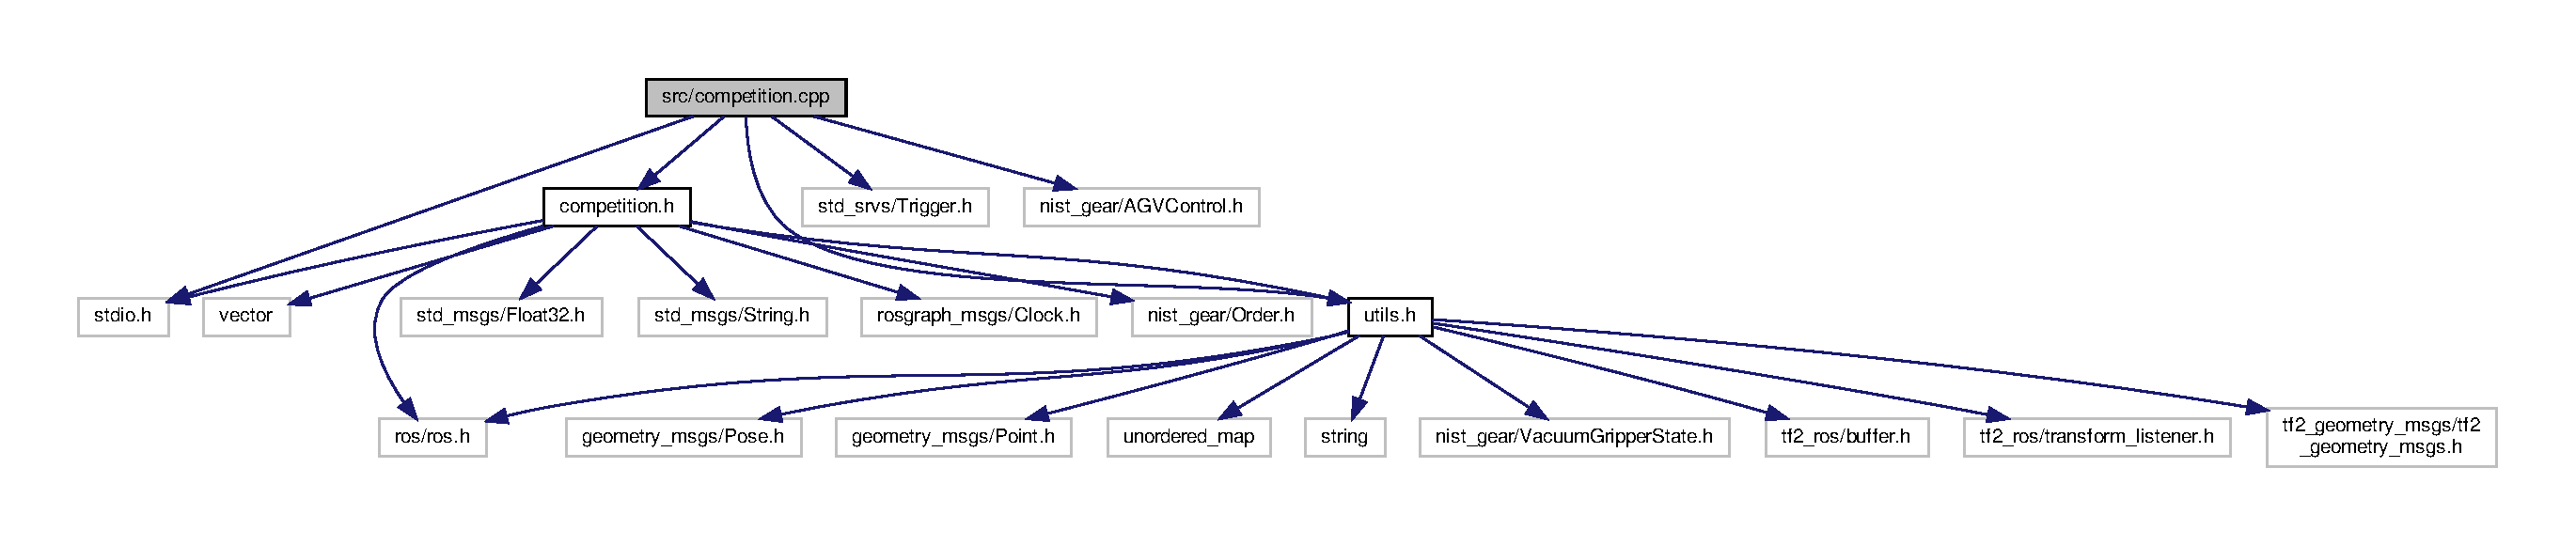
\includegraphics[width=350pt]{competition_8cpp__incl}
\end{center}
\end{figure}


\subsection{Detailed Description}
Starts the A\+R\+I\+AC competition. 

Copyright 2020 Nalin Das

\begin{DoxyAuthor}{Author}
Varun Asthana 

Saumil Shah 

Nalin Das 

Markose Jacob 

Aditya Goswami
\end{DoxyAuthor}
\begin{DoxyDate}{Date}
11/28/2020
\end{DoxyDate}
\hypertarget{utils_8cpp_DESCRIPTION}{}\subsection{D\+E\+S\+C\+R\+I\+P\+T\+I\+ON}\label{utils_8cpp_DESCRIPTION}
Source file for A\+R\+I\+AC competition class 
\hypertarget{gantry__control_8cpp}{}\section{src/gantry\+\_\+control.cpp File Reference}
\label{gantry__control_8cpp}\index{src/gantry\+\_\+control.\+cpp@{src/gantry\+\_\+control.\+cpp}}


Implements the \hyperlink{classGantryControl}{Gantry\+Control} class methods.  


{\ttfamily \#include \char`\"{}gantry\+\_\+control.\+h\char`\"{}}\newline
{\ttfamily \#include $<$tf2/\+Linear\+Math/\+Quaternion.\+h$>$}\newline
{\ttfamily \#include $<$tf2\+\_\+ros/transform\+\_\+broadcaster.\+h$>$}\newline
{\ttfamily \#include $<$tf2\+\_\+ros/static\+\_\+transform\+\_\+broadcaster.\+h$>$}\newline
{\ttfamily \#include $<$geometry\+\_\+msgs/\+Transform\+Stamped.\+h$>$}\newline
{\ttfamily \#include $<$nist\+\_\+gear/\+Logical\+Camera\+Image.\+h$>$}\newline
{\ttfamily \#include \char`\"{}utils.\+h\char`\"{}}\newline
{\ttfamily \#include \char`\"{}order\+Build.\+h\char`\"{}}\newline
{\ttfamily \#include \char`\"{}conveyer.\+h\char`\"{}}\newline
{\ttfamily \#include \char`\"{}obstacles.\+h\char`\"{}}\newline
Include dependency graph for gantry\+\_\+control.\+cpp\+:\nopagebreak
\begin{figure}[H]
\begin{center}
\leavevmode
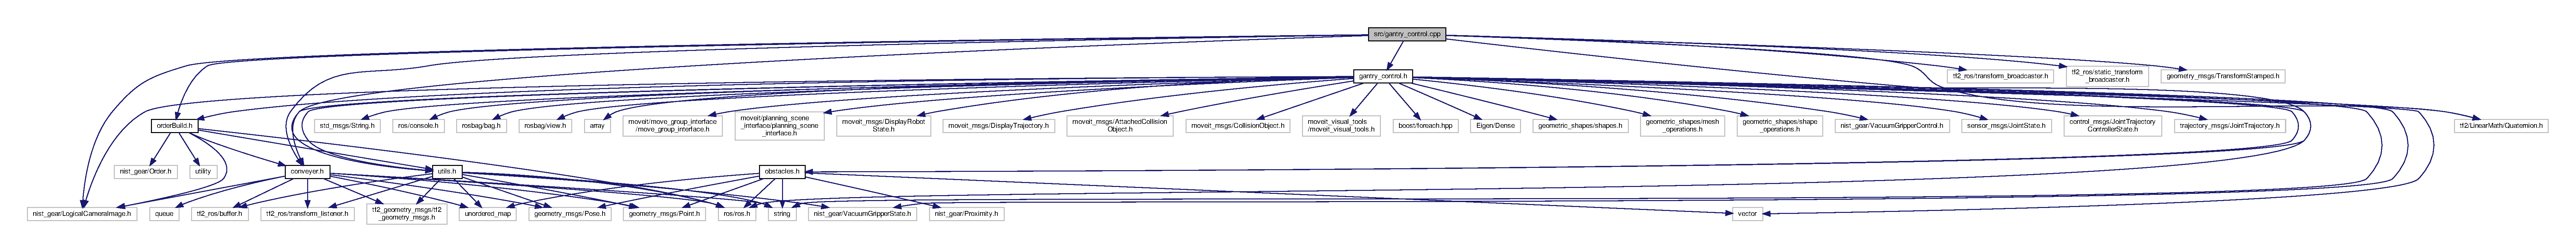
\includegraphics[width=350pt]{gantry__control_8cpp__incl}
\end{center}
\end{figure}
\subsection*{Functions}
\begin{DoxyCompactItemize}
\item 
\mbox{\Hypertarget{gantry__control_8cpp_a38b80198a6f7382fea1b64bb72f8d221}\label{gantry__control_8cpp_a38b80198a6f7382fea1b64bb72f8d221}} 
float {\bfseries get\+Dis} (const geometry\+\_\+msgs\+::\+Pose \&p1, const geometry\+\_\+msgs\+::\+Pose \&p2)
\end{DoxyCompactItemize}


\subsection{Detailed Description}
Implements the \hyperlink{classGantryControl}{Gantry\+Control} class methods. 

Copyright 2020 Nalin Das

\begin{DoxyAuthor}{Author}
Varun Asthana 

Saumil Shah 

Nalin Das 

Markose Jacob 

Aditya Goswami
\end{DoxyAuthor}
\begin{DoxyDate}{Date}
11/28/2020
\end{DoxyDate}
\hypertarget{utils_8cpp_DESCRIPTION}{}\subsection{D\+E\+S\+C\+R\+I\+P\+T\+I\+ON}\label{utils_8cpp_DESCRIPTION}
Source file for the \hyperlink{classGantryControl}{Gantry\+Control} class methods 
\hypertarget{obstacles_8cpp}{}\section{src/obstacles.cpp File Reference}
\label{obstacles_8cpp}\index{src/obstacles.\+cpp@{src/obstacles.\+cpp}}


\hyperlink{classObstaclesInAisle}{Obstacles\+In\+Aisle} class methods implementation.  


{\ttfamily \#include $<$algorithm$>$}\newline
{\ttfamily \#include $<$vector$>$}\newline
{\ttfamily \#include $<$string$>$}\newline
{\ttfamily \#include $<$unordered\+\_\+map$>$}\newline
{\ttfamily \#include $<$geometry\+\_\+msgs/\+Pose.\+h$>$}\newline
{\ttfamily \#include $<$nist\+\_\+gear/\+Proximity.\+h$>$}\newline
{\ttfamily \#include \char`\"{}competition.\+h\char`\"{}}\newline
{\ttfamily \#include $<$ros/ros.\+h$>$}\newline
{\ttfamily \#include \char`\"{}obstacles.\+h\char`\"{}}\newline
Include dependency graph for obstacles.\+cpp\+:\nopagebreak
\begin{figure}[H]
\begin{center}
\leavevmode
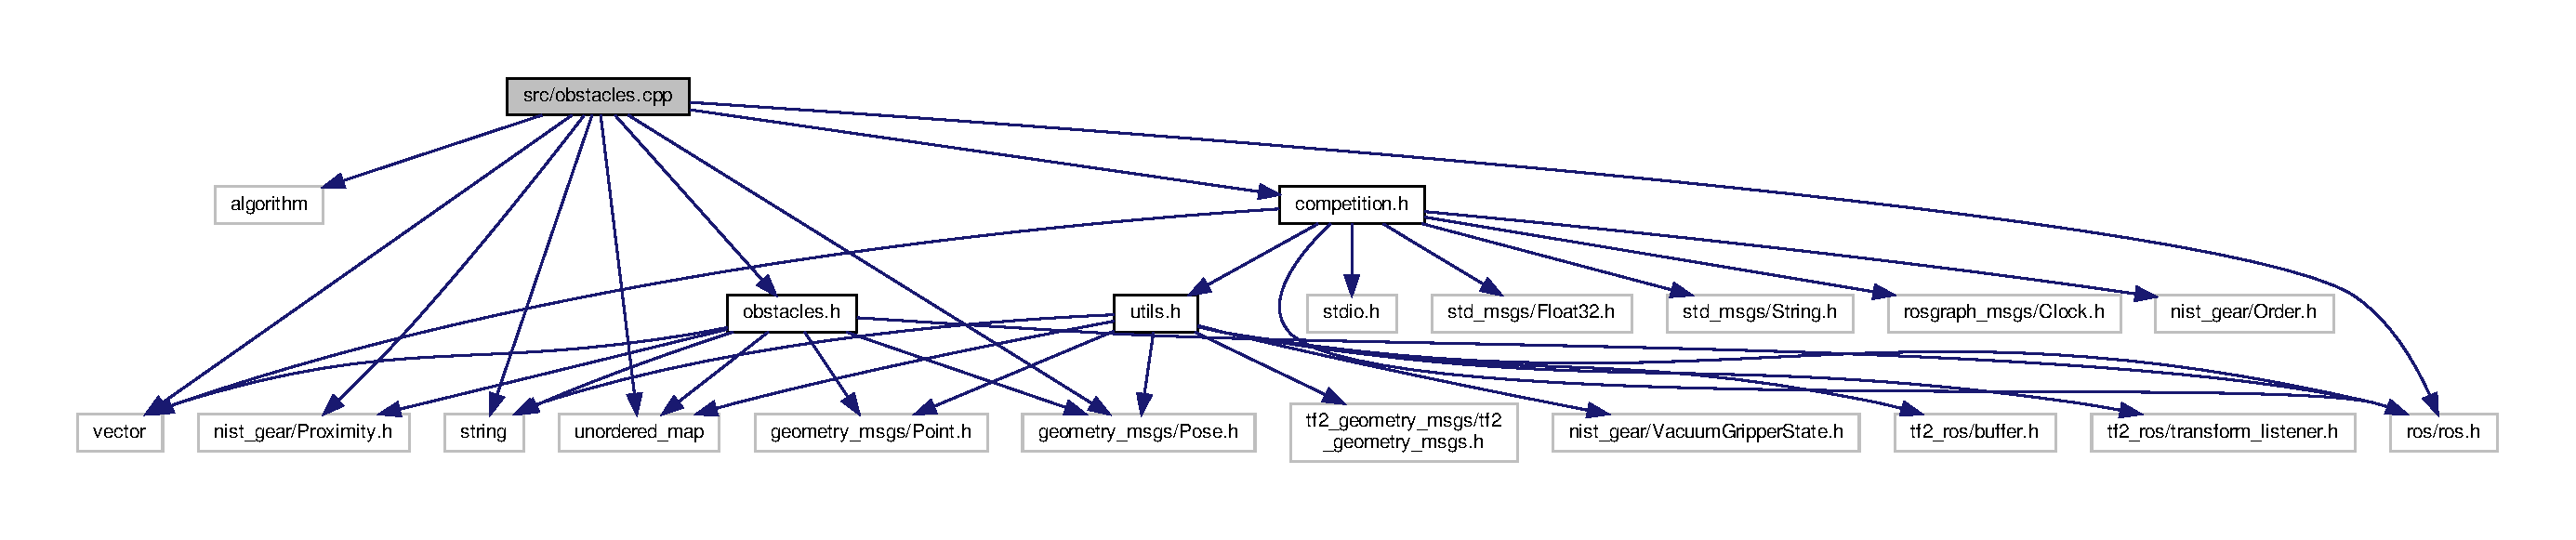
\includegraphics[width=350pt]{obstacles_8cpp__incl}
\end{center}
\end{figure}


\subsection{Detailed Description}
\hyperlink{classObstaclesInAisle}{Obstacles\+In\+Aisle} class methods implementation. 

Copyright 2020 Varun Asthana, Saumil Shah, Nalin Das, Markose Jacob, Aditya Goswami

\begin{DoxyAuthor}{Author}
Varun Asthana 

Saumil Shah 

Nalin Das 

Markose Jacob 

Aditya Goswami
\end{DoxyAuthor}
\begin{DoxyDate}{Date}
11/29/2020
\end{DoxyDate}
\hypertarget{utils_8cpp_DESCRIPTION}{}\subsection{D\+E\+S\+C\+R\+I\+P\+T\+I\+ON}\label{utils_8cpp_DESCRIPTION}
Source file for the \hyperlink{classObstaclesInAisle}{Obstacles\+In\+Aisle} class methods 
\hypertarget{orderBuild_8cpp}{}\section{src/order\+Build.cpp File Reference}
\label{orderBuild_8cpp}\index{src/order\+Build.\+cpp@{src/order\+Build.\+cpp}}


\hyperlink{classBuildClass}{Build\+Class} and \hyperlink{classallStaticParts}{all\+Static\+Parts} class implementation.  


{\ttfamily \#include \char`\"{}order\+Build.\+h\char`\"{}}\newline
{\ttfamily \#include $<$unordered\+\_\+map$>$}\newline
{\ttfamily \#include \char`\"{}conveyer.\+h\char`\"{}}\newline
{\ttfamily \#include \char`\"{}utils.\+h\char`\"{}}\newline
{\ttfamily \#include $<$utility$>$}\newline
Include dependency graph for order\+Build.\+cpp\+:
\nopagebreak
\begin{figure}[H]
\begin{center}
\leavevmode
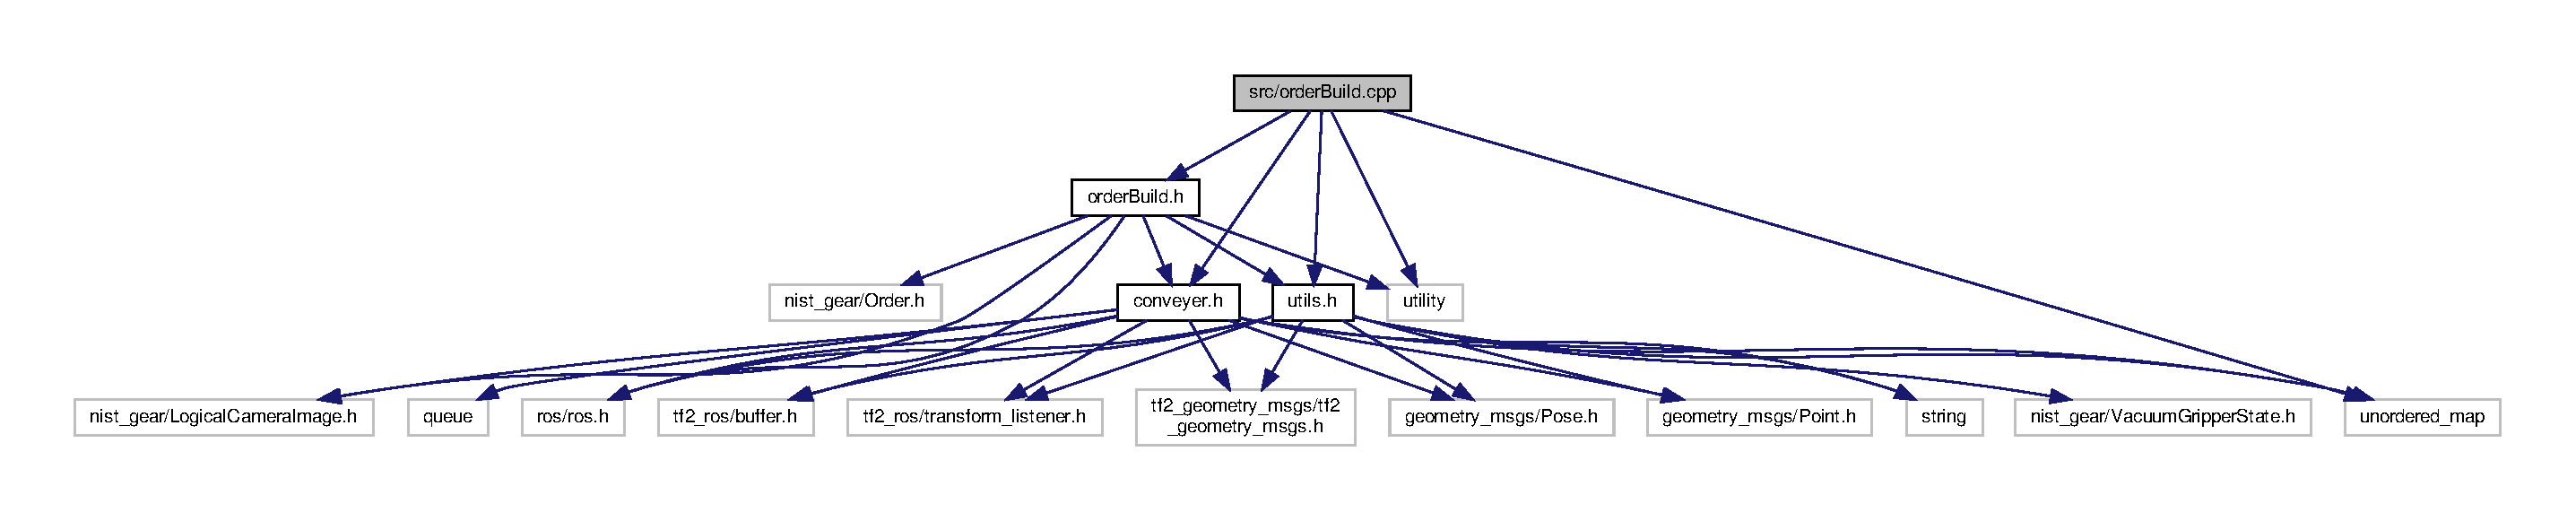
\includegraphics[width=350pt]{orderBuild_8cpp__incl}
\end{center}
\end{figure}
\subsection*{Functions}
\begin{DoxyCompactItemize}
\item 
\mbox{\Hypertarget{orderBuild_8cpp_a9745c9827a32657b845ccd2c75abb72b}\label{orderBuild_8cpp_a9745c9827a32657b845ccd2c75abb72b}} 
float {\bfseries shelf\+Dis} (const std\+::string \&name1, const std\+::string \&name2, float \&leg\+\_\+x)
\item 
\mbox{\Hypertarget{orderBuild_8cpp_a6ea8e51dde16555bbdde6b399ad2d344}\label{orderBuild_8cpp_a6ea8e51dde16555bbdde6b399ad2d344}} 
float {\bfseries shelf\+Dis\+Corner} (const std\+::string \&name1, float corner\+\_\+x)
\end{DoxyCompactItemize}


\subsection{Detailed Description}
\hyperlink{classBuildClass}{Build\+Class} and \hyperlink{classallStaticParts}{all\+Static\+Parts} class implementation. 

Copyright 2020 Varun Asthana, Saumil Shah, Nalin Das, Markose Jacob, Aditya Goswami

\begin{DoxyAuthor}{Author}
Varun Asthana 

Saumil Shah 

Nalin Das 

Markose Jacob 

Aditya Goswami
\end{DoxyAuthor}
\begin{DoxyDate}{Date}
11/29/2020
\end{DoxyDate}
\hypertarget{utils_8cpp_DESCRIPTION}{}\subsection{D\+E\+S\+C\+R\+I\+P\+T\+I\+ON}\label{utils_8cpp_DESCRIPTION}
Source file for \hyperlink{classBuildClass}{Build\+Class} and \hyperlink{classallStaticParts}{all\+Static\+Parts} class methods implementation 
\hypertarget{rwa__final__node_8cpp}{}\section{src/rwa\+\_\+final\+\_\+node.cpp File Reference}
\label{rwa__final__node_8cpp}\index{src/rwa\+\_\+final\+\_\+node.\+cpp@{src/rwa\+\_\+final\+\_\+node.\+cpp}}


Main file for rwa5.  


{\ttfamily \#include $<$algorithm$>$}\newline
{\ttfamily \#include $<$vector$>$}\newline
{\ttfamily \#include $<$string$>$}\newline
{\ttfamily \#include $<$unordered\+\_\+map$>$}\newline
{\ttfamily \#include $<$ros/ros.\+h$>$}\newline
{\ttfamily \#include $<$nist\+\_\+gear/\+Logical\+Camera\+Image.\+h$>$}\newline
{\ttfamily \#include $<$nist\+\_\+gear/\+Order.\+h$>$}\newline
{\ttfamily \#include $<$nist\+\_\+gear/\+Proximity.\+h$>$}\newline
{\ttfamily \#include $<$sensor\+\_\+msgs/\+Laser\+Scan.\+h$>$}\newline
{\ttfamily \#include $<$sensor\+\_\+msgs/\+Range.\+h$>$}\newline
{\ttfamily \#include $<$std\+\_\+msgs/\+Float32.\+h$>$}\newline
{\ttfamily \#include $<$std\+\_\+msgs/\+String.\+h$>$}\newline
{\ttfamily \#include $<$std\+\_\+srvs/\+Trigger.\+h$>$}\newline
{\ttfamily \#include $<$tf2\+\_\+ros/transform\+\_\+listener.\+h$>$}\newline
{\ttfamily \#include $<$geometry\+\_\+msgs/\+Transform\+Stamped.\+h$>$}\newline
{\ttfamily \#include $<$geometry\+\_\+msgs/\+Pose.\+h$>$}\newline
{\ttfamily \#include $<$tf2\+\_\+geometry\+\_\+msgs/tf2\+\_\+geometry\+\_\+msgs.\+h$>$}\newline
{\ttfamily \#include \char`\"{}order\+Build.\+h\char`\"{}}\newline
{\ttfamily \#include \char`\"{}competition.\+h\char`\"{}}\newline
{\ttfamily \#include \char`\"{}utils.\+h\char`\"{}}\newline
{\ttfamily \#include \char`\"{}gantry\+\_\+control.\+h\char`\"{}}\newline
{\ttfamily \#include \char`\"{}conveyer.\+h\char`\"{}}\newline
{\ttfamily \#include \char`\"{}obstacles.\+h\char`\"{}}\newline
{\ttfamily \#include $<$tf2/\+Linear\+Math/\+Quaternion.\+h$>$}\newline
{\ttfamily \#include $<$ros/console.\+h$>$}\newline
Include dependency graph for rwa\+\_\+final\+\_\+node.\+cpp\+:\nopagebreak
\begin{figure}[H]
\begin{center}
\leavevmode

\includegraphics[width=350pt]{rwa__final__node_8cpp__incl}
\end{center}
\end{figure}
\subsection*{Functions}
\begin{DoxyCompactItemize}
\item 
\mbox{\Hypertarget{rwa__final__node_8cpp_a6faa06a80398aa1570604fbf8098b15e}\label{rwa__final__node_8cpp_a6faa06a80398aa1570604fbf8098b15e}} 
void {\bfseries clock\+Callback} (const std\+\_\+msgs\+::\+String\+::\+Const\+Ptr \&msg)
\item 
\mbox{\Hypertarget{rwa__final__node_8cpp_a3c04138a5bfe5d72780bb7e82a18e627}\label{rwa__final__node_8cpp_a3c04138a5bfe5d72780bb7e82a18e627}} 
int {\bfseries main} (int argc, char $\ast$$\ast$argv)
\end{DoxyCompactItemize}


\subsection{Detailed Description}
Main file for rwa5. 

Copyright 2020 Varun Asthana, Saumil Shah, Nalin Das, Markose Jacob, Aditya Goswami

\begin{DoxyAuthor}{Author}
Varun Asthana 

Saumil Shah 

Nalin Das 

Markose Jacob 

Aditya Goswami
\end{DoxyAuthor}
\begin{DoxyDate}{Date}
11/29/2020 
\end{DoxyDate}
\hypertarget{utils_8cpp_DESCRIPTION}{}\subsection{D\+E\+S\+C\+R\+I\+P\+T\+I\+ON}\label{utils_8cpp_DESCRIPTION}
Source main file for rwa5 
\hypertarget{utils_8cpp}{}\section{src/utils.cpp File Reference}
\label{utils_8cpp}\index{src/utils.\+cpp@{src/utils.\+cpp}}


Utility functions implementation.  


{\ttfamily \#include \char`\"{}utils.\+h\char`\"{}}\newline
{\ttfamily \#include $<$geometry\+\_\+msgs/\+Pose.\+h$>$}\newline
Include dependency graph for utils.\+cpp\+:
\nopagebreak
\begin{figure}[H]
\begin{center}
\leavevmode
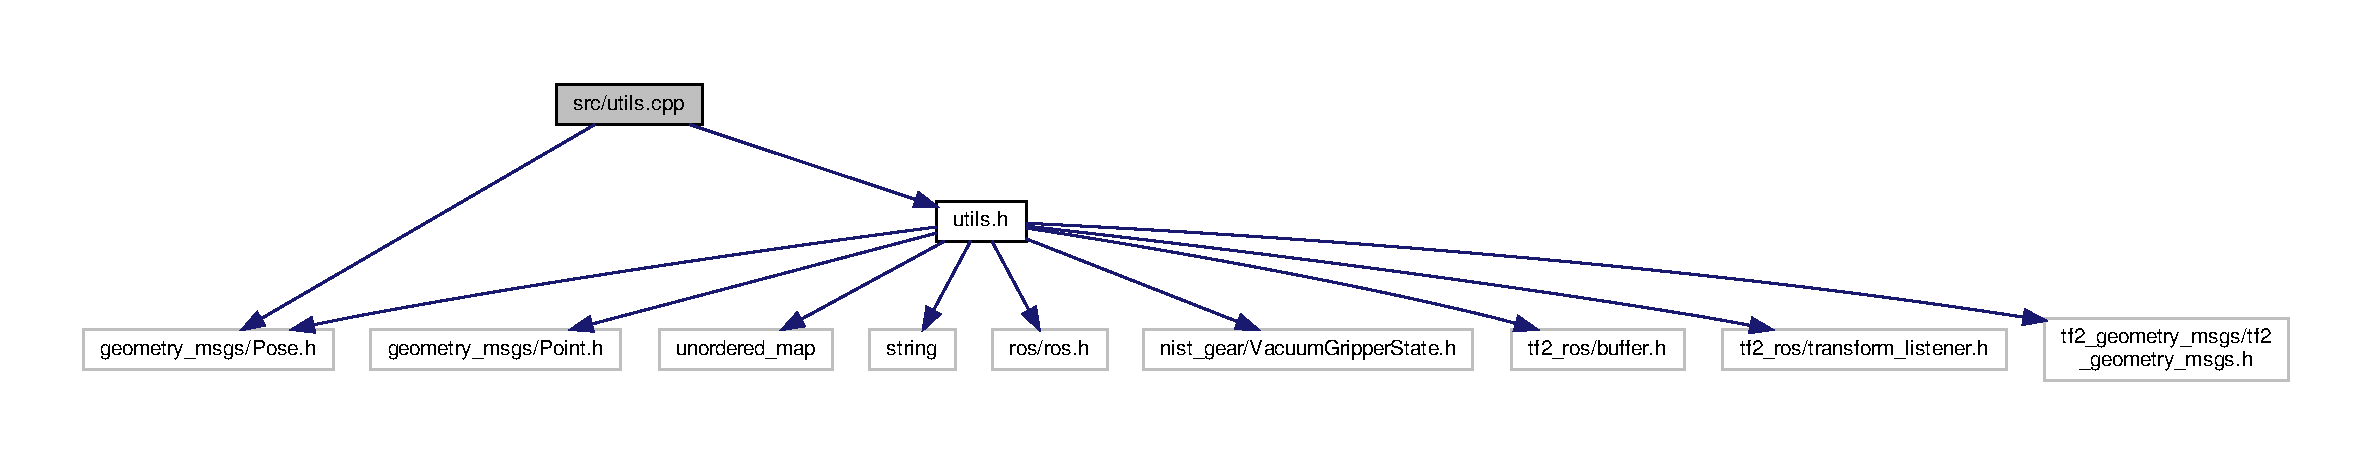
\includegraphics[width=350pt]{utils_8cpp__incl}
\end{center}
\end{figure}
\subsection*{Functions}
\begin{DoxyCompactItemize}
\item 
std\+::vector$<$ double $>$ \hyperlink{utils_8cpp_a6296f07aa6ba20f987431f971ffd77b9}{quaternion\+To\+Euler} (geometry\+\_\+msgs\+::\+Pose pose)
\begin{DoxyCompactList}\small\item\em Quaternion To Euler function. \end{DoxyCompactList}\end{DoxyCompactItemize}
\subsection*{Variables}
\begin{DoxyCompactItemize}
\item 
std\+::unordered\+\_\+map$<$ std\+::string, double $>$ \hyperlink{utils_8cpp_a4443f04d04826b4cb4d695dadc9a3a03}{model\+\_\+height}
\begin{DoxyCompactList}\small\item\em Model height hashmap. \end{DoxyCompactList}\end{DoxyCompactItemize}


\subsection{Detailed Description}
Utility functions implementation. 

Copyright 2020 Varun Asthana, Saumil Shah, Nalin Das, Markose Jacob, Aditya Goswami

\begin{DoxyAuthor}{Author}
Varun Asthana 

Saumil Shah 

Nalin Das 

Markose Jacob 

Aditya Goswami
\end{DoxyAuthor}
\begin{DoxyDate}{Date}
11/29/2020
\end{DoxyDate}
\hypertarget{utils_8cpp_DESCRIPTION}{}\subsection{D\+E\+S\+C\+R\+I\+P\+T\+I\+ON}\label{utils_8cpp_DESCRIPTION}
Source file for Utility functions implementation. 

\subsection{Function Documentation}
\mbox{\Hypertarget{utils_8cpp_a6296f07aa6ba20f987431f971ffd77b9}\label{utils_8cpp_a6296f07aa6ba20f987431f971ffd77b9}} 
\index{utils.\+cpp@{utils.\+cpp}!quaternion\+To\+Euler@{quaternion\+To\+Euler}}
\index{quaternion\+To\+Euler@{quaternion\+To\+Euler}!utils.\+cpp@{utils.\+cpp}}
\subsubsection{\texorpdfstring{quaternion\+To\+Euler()}{quaternionToEuler()}}
{\footnotesize\ttfamily std\+::vector$<$double$>$ quaternion\+To\+Euler (\begin{DoxyParamCaption}\item[{geometry\+\_\+msgs\+::\+Pose}]{pose }\end{DoxyParamCaption})}



Quaternion To Euler function. 


\begin{DoxyParams}{Parameters}
{\em pose} & Quaternion pose \\
\hline
\end{DoxyParams}
\begin{DoxyReturn}{Returns}
Converted Euler angles 
\end{DoxyReturn}


\subsection{Variable Documentation}
\mbox{\Hypertarget{utils_8cpp_a4443f04d04826b4cb4d695dadc9a3a03}\label{utils_8cpp_a4443f04d04826b4cb4d695dadc9a3a03}} 
\index{utils.\+cpp@{utils.\+cpp}!model\+\_\+height@{model\+\_\+height}}
\index{model\+\_\+height@{model\+\_\+height}!utils.\+cpp@{utils.\+cpp}}
\subsubsection{\texorpdfstring{model\+\_\+height}{model\_height}}
{\footnotesize\ttfamily std\+::unordered\+\_\+map$<$std\+::string, double$>$ model\+\_\+height}

{\bfseries Initial value\+:}
\begin{DoxyCode}
= \{
        \{\textcolor{stringliteral}{"piston\_rod\_part\_red"}, 0.0065\}, 
        \{\textcolor{stringliteral}{"piston\_rod\_part\_green"}, 0.0065\},
        \{\textcolor{stringliteral}{"piston\_rod\_part\_blue"}, 0.0065\},
        \{\textcolor{stringliteral}{"pulley\_part\_red"}, 0.07\},
        \{\textcolor{stringliteral}{"pulley\_part\_green"}, 0.07\},
        \{\textcolor{stringliteral}{"pulley\_part\_blue"}, 0.07\},
        \{\textcolor{stringliteral}{"gear\_part\_red"}, 0.012\},
        \{\textcolor{stringliteral}{"gear\_part\_green"}, 0.012\},
        \{\textcolor{stringliteral}{"gear\_part\_blue"}, 0.012\},
        \{\textcolor{stringliteral}{"gasket\_part\_red"}, 0.03\},
        \{\textcolor{stringliteral}{"gasket\_part\_green"}, 0.03\},
        \{\textcolor{stringliteral}{"gasket\_part\_blue"}, 0.03\},
        \{\textcolor{stringliteral}{"disk\_part\_red"}, 0.023\},
        \{\textcolor{stringliteral}{"disk\_part\_green"}, 0.023\},
        \{\textcolor{stringliteral}{"disk\_part\_blue"}, 0.023\}
\}
\end{DoxyCode}


Model height hashmap. 


%--- End generated contents ---

% Index
\backmatter
\newpage
\phantomsection
\clearemptydoublepage
\addcontentsline{toc}{chapter}{Index}
\printindex

\end{document}
